\documentclass[a4paper,11pt,oneside]{article}

\usepackage[utf8]{inputenc}
\usepackage[T1]{fontenc}
\usepackage[a4paper,top=3cm,bottom=3cm,left=3cm,right=3cm]{geometry}
\renewcommand{\familydefault}{\sfdefault}
\usepackage{helvet}
\usepackage[english]{babel}
\usepackage[style=numeric,language=english]{biblatex}
\usepackage{parskip}
\usepackage[margin=1cm]{caption}
\usepackage{booktabs}
\usepackage{multirow}
\usepackage[cache=false]{minted}
\usepackage{listings}
\usepackage{xcolor}
\usepackage{upquote}
\definecolor{lstkw}{RGB}{0,80,160}
\definecolor{lstcomment}{RGB}{96,128,96}
\definecolor{lststr}{RGB}{160,32,32}
\definecolor{lstbg}{RGB}{248,248,248}
\lstdefinestyle{pythonstyle}{
  language=Python,
  basicstyle=\ttfamily\footnotesize,
  keywordstyle=\color{lstkw}\bfseries,
  commentstyle=\color{lstcomment}\itshape,
  stringstyle=\color{lststr},
  backgroundcolor=\color{lstbg},
  showstringspaces=false,
  upquote=true,
  breaklines=true,
  breakatwhitespace=true,
  frame=single,
  framesep=4pt,
  rulecolor=\color{black!20},
  xleftmargin=0.5em,
  xrightmargin=0.5em,
  numbers=left,
  numberstyle=\tiny\color{black!50},
  numbersep=6pt,
  captionpos=b,
  literate={—}{{---}}1 {–}{{--}}1
}
\lstset{style=pythonstyle}
\usepackage{csquotes}
\usepackage{amsmath}
\usepackage{amssymb}
\usepackage{amsthm}
\newtheoremstyle{breakstyle}%
  {1em}          % above space
  {0.6em}        % below space
  {\normalfont}  % body font (no italic)
  {0pt}          % indent
  {\bfseries}    % head font
  {.}            % punctuation after head
  {\newline}     % space (newline) after head
  {}             % default head spec
\theoremstyle{breakstyle}
\newtheorem{lemma}{Lemma}[section]
\newtheorem{corollary}[lemma]{Corollary}
\usepackage[pdftex]{graphicx}
\graphicspath{{./}{../slides/figs/}{../slides_v2/figs/}}
\usepackage{epstopdf}
\usepackage{tikz}
\usetikzlibrary{arrows.meta}
\definecolor{myblue}{HTML}{2E86AB}
\definecolor{myorange}{HTML}{E07A5F}
\definecolor{mybluedark}{HTML}{1A5276}
\definecolor{mygreen}{HTML}{3D9970}
\definecolor{myred}{HTML}{C0392B}
\usepackage[pdftex]{hyperref}
\pdfadjustspacing=1

\newcommand{\mylastname}{Burykina}
\newcommand{\myfirstname}{Alina}
\newcommand{\mynumber}{30008248}
\newcommand{\myname}{\myfirstname{} \mylastname{}}
\newcommand{\mytitle}{ADC-Aware Quantization of Large Language Models for In-Memory Computing}
\newcommand{\mysupervisor}{Prof.~Dr.~Dmitry Vetrov}

\hypersetup{
  pdfauthor = {\myname},
  pdftitle = {\mytitle},
  pdfkeywords = {LLaMA, quantization, in-memory computing, ADC, FlatQuant, post-training quantization},
  colorlinks = {true},
  linkcolor = {blue}
}

\addbibresource{msc-sample.bib}
\setcounter{tocdepth}{2}

\begin{document}
  \pagenumbering{roman}

  \thispagestyle{empty}

  \begin{flushright}
    
\includegraphics[scale=0.8]{msc-logo}
  \end{flushright}
  \vspace*{40mm}
  \begin{center}
    \huge
    \textbf{\mytitle}
  \end{center}
  \vspace*{4mm}
  \begin{center}
   \Large by
  \end{center}
  \vspace*{4mm}
  \begin{center}
    \LARGE
    \textbf{\myname}
  \end{center}
  \vspace*{20mm}
  \begin{center}
    \Large
    Master Thesis in Computer Science and Software Engineering
  \end{center}
  \vfill
  \begin{flushleft}
    \large
    Submission: \today \hfill Supervisor: \mysupervisor \\
    \rule{\textwidth}{1pt}
  \end{flushleft}
  \begin{center}
    Constructor University $|$ Constructor Institute of Technology
  \end{center}

  \newpage
  \thispagestyle{empty}

  \begin{center}
    \Large \textbf{Statutory Declaration}
    \vspace*{8mm}
  \end{center}

  \begin{center}
    \begin{tabular}{|l|p{85mm}|}
      \hline
      Family Name, Given/First Name & \mylastname, \myfirstname \\
      Matriculation number & \mynumber \\
      Kind of thesis submitted & Master Thesis \\
      \hline
    \end{tabular}
    \vspace*{8mm}
  \end{center}

  \subsection*{English: Declaration of Authorship}
 
  I hereby declare that the thesis submitted was created and written
  solely by myself without any external support. Any sources, direct
  or indirect, are marked as such. I am aware of the fact that the
  contents of the thesis in digital form may be revised with regard to
  usage of unauthorized aid as well as whether the whole or parts of
  it may be identified as plagiarism. I do agree my work to be entered
  into a database for it to be compared with existing sources, where
  it will remain in order to enable further comparisons with future
  theses. This does not grant any rights of reproduction and usage,
  however.

  This document was neither presented to any other examination board
  nor has it been published.

  \subsection*{German: Erklärung der Autorenschaft (Urheberschaft)}
 
  Ich erkläre hiermit, dass die vorliegende Arbeit ohne fremde Hilfe
  ausschließlich von mir erstellt und geschrieben worden ist. Jedwede
  verwendeten Quellen, direkter oder indirekter Art, sind als solche
  kenntlich gemacht worden. Mir ist die Tatsache bewusst, dass der
  Inhalt der Thesis in digitaler Form geprüft werden kann im Hinblick
  darauf, ob es sich ganz oder in Teilen um ein Plagiat handelt. Ich
  bin damit einverstanden, dass meine Arbeit in einer Datenbank
  eingegeben werden kann, um mit bereits bestehenden Quellen
  verglichen zu werden und dort auch verbleibt, um mit zukünftigen
  Arbeiten verglichen werden zu können. Dies berechtigt jedoch nicht
  zur Verwendung oder Vervielfältigung.

  Diese Arbeit wurde noch keiner anderen Prüfungsbehörde vorgelegt
  noch wurde sie bisher veröffentlicht.

  \vspace{20mm}

  \dotfill\\
  Date, Signature

  \newpage

  \section*{Abstract}
  \addcontentsline{toc}{section}{Abstract}

  Analog optical matrix-vector accelerators promise energy-efficient
  inference for large language models (LLMs), but they expose a
  failure mode absent from standard digital deployment: after each
  analog accumulation, a finite-resolution analog-to-digital
  converter (ADC) maps the output onto a hardware-fixed quantization
  lattice. This post-accumulation quantizer is especially damaging
  for large language models, whose channel-wise outliers make a
  single ADC scale difficult to use. Previous hardware-aware
  approaches commonly rely on retraining through the hardware model;
  for billion-parameter large language models, such
  quantization-aware training is often impractical because the
  original training data and compute budget are unavailable.

  This thesis instead investigates whether an already trained large
  language model can be adapted in the post-training setting.
  Building on FlatQuant, an ADC-aware post-training quantization
  (PTQ) pipeline is introduced in which calibration is made to match
  analog inference by propagating ADC-quantized activations across
  blocks, mixing clean and ADC-aware objectives, and applying
  bounded diagonal scaling with staged calibration. On Llama-3.2-1B
  in the 4-bit weight and 4-bit activation (W4A4) setting, standard
  FlatQuant remains usable when the ADC is disabled, with WikiText-2
  perplexity $15.41$, but collapses when the ADC is enabled,
  reaching $2354$. ADC-aware post-training quantization reduces this
  to $26.66$, showing that transform-based calibration is necessary
  but plateaus far from the bfloat16 baseline of $8.68$.

  To close the remaining gap without full quantization-aware
  training, a rank-4 digital residual branch is added after the ADC,
  and only this low-rank correction is trained using cross-entropy
  and teacher Kullback--Leibler distillation. This
  $0.22\%$-parameter adaptation reduces WikiText-2/C4 ADC perplexity
  from $26.66/45.62$ to $\mathbf{14.03}/\mathbf{23.20}$. These
  results show that fixed low-resolution ADCs require algorithmic
  adaptation beyond digital post-training quantization, and that
  lightweight output-side digital correction can recover much of the
  accuracy lost at the analog-digital boundary.

  \newpage
  \tableofcontents

  \clearpage
  \pagenumbering{arabic}


  \section{Introduction}
\label{sec:introduction}

Large language models (LLMs) have become the dominant architecture for
modern natural language processing (NLP), but their inference cost remains a
major deployment obstacle. Transformer decoders are built primarily from
large matrix--vector and matrix--matrix multiplications, and serving them
requires repeatedly moving weights and activations between memory and
compute units. In fact, autoregressive decoding is already
memory-bandwidth-bound on modern GPUs: each forward pass reads
billions of parameters to produce only a single output token, so the
arithmetic intensity falls far below the hardware roofline and
throughput is limited by memory bandwidth rather than compute
\cite{Pope2023EfficientlyScaling}. This motivates hardware architectures
that mitigate the data movement bottleneck by moving the dominant
matrix--vector multiplications closer to memory, including in-memory
computing (IMC) accelerators, where matrix--vector multiplication
can be performed directly inside memory arrays rather than in a
conventional digital compute core \cite{Xiao2021AnalogAccuracy,LeGallo2023AnalogNAS,
Buechel2025AnalogFoundation}.

IMC is attractive for LLM inference because transformer layers are
dominated by linear projections. In an idealized IMC pipeline, the weight
matrix of a projection is stored in a memory array, an input activation
vector is applied to the array, and the analog accumulation implements
the dot product. However, this analog result must be converted back into
a digital value before it can be consumed by the next layer, placing the
analog-to-digital converter (ADC) directly on the neural network
inference path. The precision and range of the ADC therefore determine
how much information from the analog accumulation is preserved.

This thesis studies the interaction between transformer quantization and
ADC-constrained analog inference. In a conventional digital quantization
setting, the main sources of error are weight and activation quantization.
In an IMC accelerator there is an additional output quantization stage:
the accumulated analog result is passed through the ADC, which
quantizes it to a fixed step size $\Delta$ and clips it to the
ADC output range. The central difference from digital low-bit inference
is that even if weights and activations are quantized well, the
accumulated output can still be severely distorted by a coarse ADC
lattice.

Unlike the activation and weight scales, which are adjusted during
calibration, the ADC step size $\Delta$ is fixed by the analog hardware
at design time and cannot be reduced by retraining or by changing the
learned quantization transform. The only software-side levers available
are how the signal is shaped before the ADC and how the quantized output
is corrected after it. This makes ADC-constrained inference a different
optimization problem from standard digital PTQ.

LLMs are a particularly challenging target for this setting. Prior work
has shown that transformer activations contain large outlier channels,
and that these outliers are a major obstacle to low-bit quantization
\cite{LLMint82022,SmoothQuant2022,OutlierSuppressionPlus2023,
QuaRot2024,SpinQuant2024}. Because activation scales are computed from
the per-token maximum, a single large channel sets the scale for the
entire activation vector. Typical activation values then receive very small integer
codes, reducing the effective density of the integer dot product. In an
ADC pipeline this can produce poorly occupied ADC bins or dead regions
where small accumulated outputs collapse to zero. LLM activation
outliers therefore affect both activation quantization and the
quality of the analog output seen by the ADC.

This thesis focuses on decoder-only transformer LLMs,
using Llama-3.2-1B as the main experimental target. The goal is to study
whether transform-based post-training quantization (PTQ), combined with
ADC-aware calibration and lightweight adaptation, can make low-bit
LLaMA inference viable under ADC-constrained analog computation. The
work starts from FlatQuant, a transform-based PTQ method that learns
layer-wise affine transformations to make weights and activations easier
to quantize \cite{FlatQuant2024}. FlatQuant changes the coordinate
system in which quantization is applied while leaving the linear map
unchanged. The transformed activation distribution is flatter, so
per-token scaling is no longer dominated by a few outlier channels.

Standard PTQ methods optimize for digital quantization and do not account
for ADC output discretization as a separate source of error. Even with
well-calibrated weights and activations, ADC-path perplexity remains
substantially higher than no-ADC perplexity, the quality achievable
with digital quantization alone. Closing this gap requires calibration
that is explicitly sensitive to ADC noise and, ultimately, a lightweight
correction stage applied after the ADC path.
This thesis makes the following contributions:
\begin{enumerate}
    \item ADC-constrained formulation for LLaMA PTQ.
    The thesis formulates LLaMA inference under a tiled ADC-constrained
    matrix--vector multiplication (MVM) model and implements a
    simulation pipeline with per-token
    activation quantization, per-channel weight quantization, integer
    accumulation, ADC output quantization, and dequantization.

    \item Diagnosis of ADC-specific failure modes.
    The thesis separates ordinary weight and activation quantization error
    from ADC output quantization error using no-ADC evaluation,
    dead-rate, ADC bin usage, reconstruction error, and layer/projection
    ablations. This shows that dead zones can be caused by poor
    transforms, but that the remaining degradation can be dominated by
    ADC output resolution.

    \item ADC-aware FlatQuant calibration.
    The thesis adapts FlatQuant to ADC-constrained inference by
    adding ADC propagation across blocks, an $\alpha$-mixing
    objective between clean and ADC-propagated reconstruction, and a
    staged calibration schedule.  For per-channel scaling, the
    method builds on the learnable scaling component already used
    in FlatQuant-style PTQ but studies its bounded form, placement
    between attention and MLP sub-layers, and interaction with
    ADC-aware calibration.  Together these adaptations reduce INT4
    ADC perplexity from 2354 (naive baseline) to $26.66$ on
    WikiText-2.

    \item Analysis of pure PTQ limitations.
    Extensive ablations show that additional dead-zone penalties,
    aggressive PACT-style clipping, fixed Hadamard initialization, and
    bin-center losses are insufficient or harmful in the studied setting.
    Pure PTQ improves substantially but eventually reaches a plateau
    beyond which further calibration yields diminishing returns.

    \item Residual post-ADC low-rank correction.
    The thesis introduces a lightweight residual correction stage on top
    of the frozen quantized ADC path, trained with distillation against
    a full-precision teacher. With only 0.22\% extra parameters, this
    stage drops INT4 ADC perplexity from 26.66 to 14.03 on WikiText-2
    and from 45.62 to 23.20 on C4, while keeping the base ADC model
    frozen.
\end{enumerate}


\section{Background and Related Work}
\label{sec:background}

\subsection{In-Memory Computing and ADC-Constrained Inference}
\label{subsec:imc_adc}

In-memory computing (IMC) executes matrix--vector multiplication (MVM)
directly inside memory arrays, reducing the cost of data movement that
dominates conventional digital inference pipelines
\cite{Xiao2021AnalogAccuracy,LeGallo2023AnalogNAS,Buechel2025AnalogFoundation}.
In crossbar-style accelerators, neural network weights are mapped to
cell conductances, the input vector is applied as an analog excitation,
and the array physics performs the accumulation. This is attractive for
large neural networks because MVM is the dominant operation in both
attention and MLP blocks. However, the result of the array is analog,
whereas the next layer expects a digital tensor. Therefore, each analog
MVM must be followed by analog-to-digital conversion (ADC).

The same analog-to-digital bottleneck appears across very different
physical substrates. Memristive and phase-change-memory crossbars
encode weights as cell conductances and exploit Ohm's law plus
Kirchhoff's current summation for the multiply--accumulate
\cite{Xiao2021AnalogAccuracy,LeGallo2023AnalogNAS,Buechel2025AnalogFoundation};
photonic systems instead encode weights and activations as light
intensities or phases and perform the MVM through optical
interference, reading the result with photodetectors
\cite{Spall2022HybridOptical}. Despite the different physics, the
common feature is that the analog accumulation is then sampled by a
finite-resolution ADC before the next layer can consume it.
Figure~\ref{fig:imc_optical_pipeline} illustrates this for the optical
case: the analog signal carrying the MVM result is converted to a
digital code through a photodetector front-end followed by an ADC,
after which it re-enters the digital data path.

\begin{figure}[htbp]
  \centering
  \begin{tikzpicture}
    \node[anchor=south west, inner sep=0] (img)
      {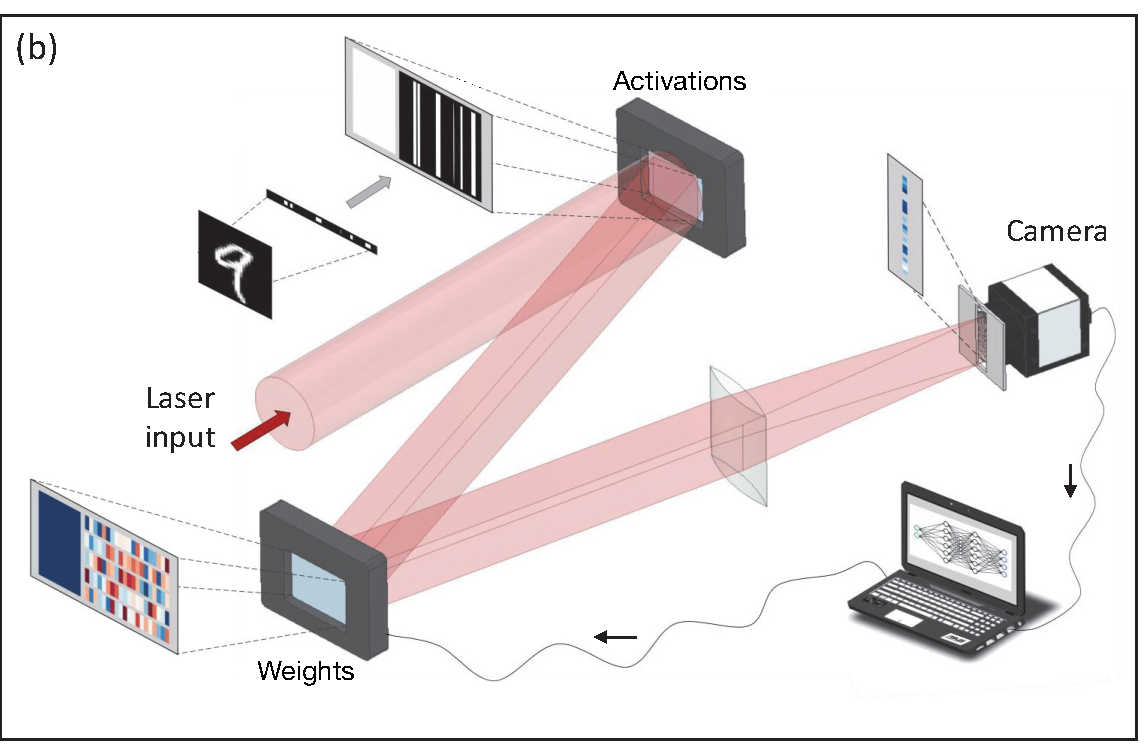
\includegraphics[width=0.95\linewidth]{Fig1b.pdf}};
    \begin{scope}[x={(img.south east)}, y={(img.north west)}]
      \fill[white] (0.013, 0.88) rectangle (0.055, 0.97);
    \end{scope}
  \end{tikzpicture}
  \caption{Physical example of an analog matrix--vector multiplication
    feeding an ADC. The figure, reproduced from Spall, Guo, and Lvovsky
    \cite{Spall2022HybridOptical}, shows an optical neural-network
    front-end: weights and activations are encoded into light fields,
    the inner product is computed by optical interference, and the
    analog accumulator output is read by a photodetector before being
    sampled by an ADC. The same analog-input--ADC-output structure
    underlies electronic in-memory computing crossbars; the
    mathematical model in
    Eqs.~\eqref{eq:adc_quantizer}--\eqref{eq:adc_delta_background}
    abstracts both.}
  \label{fig:imc_optical_pipeline}
\end{figure}

A simplified ADC-constrained inference pipeline, illustrated in
Figure~\ref{fig:analog_mvm_pipeline}, follows the math model adopted by
prior work on analog and ADC-constrained inference~\cite{RAOQ2024} and
can be written as
\begin{align}
x_q &= Q_x(x), \\
W_q &= Q_w(W), \\
y_{\mathrm{int}} &= W_q x_q, \\
y_{\mathrm{adc}} &= Q_{\mathrm{ADC}}(y_{\mathrm{int}}), \\
\hat{y} &= D_{\mathrm{out}} \, y_{\mathrm{adc}},
\end{align}
where $Q_x$ and $Q_w$ are the activation and weight quantizers,
$Q_{\mathrm{ADC}}$ denotes the output quantizer implemented by the ADC,
and $D_{\mathrm{out}}$ is the dequantization map. In the ADC model used
throughout this thesis, the analog accumulation is quantized by a
coarse output lattice:
\begin{equation}
Q_{\mathrm{ADC}}(u)
=
\Delta \cdot
\mathrm{clip}
\!\left(
\left\lfloor \frac{u}{\Delta} \right\rfloor,
n_a, p_a
\right),
\label{eq:adc_quantizer}
\end{equation}
where $\Delta$ is the ADC step size and $(n_a,p_a)$ are the output code
bounds. In a tiled IMC setting, one common hardware model yields
\begin{equation}
\Delta
=
\frac{2\,n_t\,q_x\,q_w}{2^{b_a}k},
\label{eq:adc_delta_background}
\end{equation}
where $n_t$ is the tile size, $b_a$ is the ADC bitwidth, $k$ is the ADC
scaling factor, and $q_x$, $q_w$ are the maximum activation and
weight code levels. Equation~\eqref{eq:adc_delta_background} makes the
hardware trade-off explicit: larger tiles or lower ADC precision lead to
coarser output quantization.

The scaling factor $k$ controls the trade-off between ADC resolution
and clipping. The worst-case range of the integer accumulation is
$[-n_t q_x q_w, +n_t q_x q_w]$, and the ADC covers a fraction $1/k$
of this range with $2^{b_a}$ uniform bins.

A small $k$ covers the full worst-case range at the cost of a coarse
step $\Delta$, so most of the typical pre-ADC distribution maps into a
few central codes. A large $k$ shrinks both the representable range
and the step $\Delta$ by the same factor, giving a finer lattice on
values near zero at the cost of clipping the tails. The relationship
is illustrated in Fig.~\ref{fig:k_role}.

The default hardware configuration of this thesis fixes
$n_t = 256$, $b_x = b_w = 4$, $b_a = 8$, and $k = 16$. All other hardware parameters are held fixed in this default; $k$
itself is varied in a dedicated per-layer $k$-search experiment in
Sec.~\ref{sec:unipolar}, which selects an ADC scaling factor
independently for each projection layer in the Unsigned setting.

\begin{figure}[htbp]
  \centering
  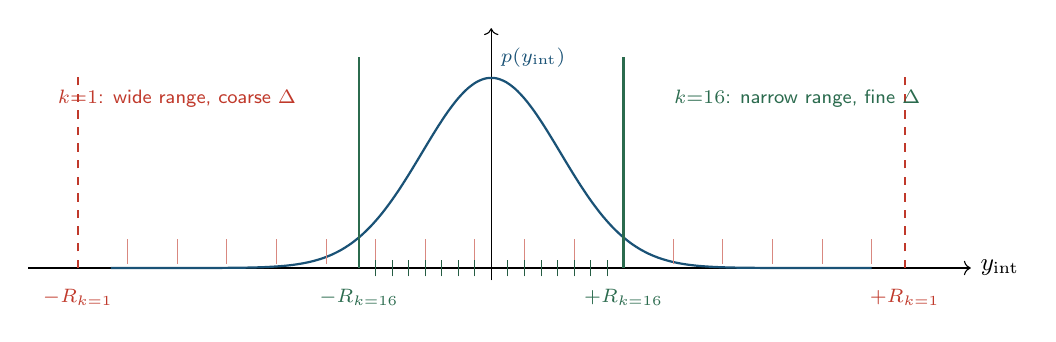
\begin{tikzpicture}[scale=1.05]
    % axes
    \draw[->] (-5.6, 0) -- (5.8, 0) node[right, font=\small] {$y_{\mathrm{int}}$};
    \draw[->] (0, -0.15) -- (0, 2.9);

    % Gaussian pre-ADC distribution
    \draw[thick, mybluedark, domain=-4.6:4.6, samples=80, smooth]
      plot (\x, {2.3*exp(-\x*\x/1.4)});
    \node at (0.0, 2.55) [right, font=\scriptsize, text=mybluedark]
      {$p(y_{\mathrm{int}})$};

    % ADC range markers for k=1 (wide, dashed red)
    \draw[dashed, thick, myred] (-5.0, 0.0) -- (-5.0, 2.4);
    \draw[dashed, thick, myred] (5.0, 0.0) -- (5.0, 2.4);
    \foreach \xx in {-4.4, -3.8, -3.2, -2.6, -2.0, -1.4, -0.8, -0.2,
                      0.4, 1.0, 1.6, 2.2, 2.8, 3.4, 4.0, 4.6} {
      \draw[myred!60, very thin] (\xx, 0.05) -- (\xx, 0.35);
    }
    \node at (-5.0, -0.35) [font=\scriptsize, text=myred]
      {$-R_{k{=}1}$};
    \node at (5.0, -0.35) [font=\scriptsize, text=myred]
      {$+R_{k{=}1}$};
    \node at (-3.8, 2.05) [font=\scriptsize, text=myred]
      {$k{=}1$: wide range, coarse $\Delta$};

    % ADC range for k=16 (narrow, solid green)
    \draw[thick, mygreen!70!black] (-1.6, 0.0) -- (-1.6, 2.55);
    \draw[thick, mygreen!70!black] (1.6, 0.0) -- (1.6, 2.55);
    \foreach \xx in {-1.4, -1.2, -1.0, -0.8, -0.6, -0.4, -0.2,
                      0.2, 0.4, 0.6, 0.8, 1.0, 1.2, 1.4} {
      \draw[mygreen!60!black, very thin] (\xx, -0.1) -- (\xx, 0.1);
    }
    \node at (-1.6, -0.35) [font=\scriptsize, text=mygreen!70!black]
      {$-R_{k{=}16}$};
    \node at (1.6, -0.35) [font=\scriptsize, text=mygreen!70!black]
      {$+R_{k{=}16}$};
    \node at (3.7, 2.05) [font=\scriptsize, text=mygreen!70!black]
      {$k{=}16$: narrow range, fine $\Delta$};
  \end{tikzpicture}
  \caption{Role of the ADC scaling factor $k$. The blue curve is the
    pre-ADC distribution of $y_{\mathrm{int}}$. The red dashed
    markers show the representable ADC range for $k = 1$: it covers
    the full worst-case range $\pm n_t q_x q_w$, but the bin width
    $\Delta$ is so wide that most of the distribution maps into a few
    central codes. The green solid markers show the same ADC for
    $k = 16$: the representable range shrinks $16\times$ but
    $\Delta$ also shrinks $16\times$, so values near zero are resolved
    with $16\times$ finer steps while values in the tails are clipped.
    This thesis uses $k = 16$.}
  \label{fig:k_role}
\end{figure}

Two failure modes follow directly from this discretisation, both
shown in Fig.~\ref{fig:dead_zone}. The dead zone is asymmetric under
floor quantization: values in $0 \le y_{\mathrm{int}} < \Delta$ map
to the zero code, whereas small negative values
$-\Delta \le y_{\mathrm{int}} < 0$ map to the $-1$ code rather than
zero. The dead-rate is therefore measured directly as the fraction of
post-ADC codes equal to zero (Eq.~\ref{eq:dead_rate}). Clipping occurs
when $|y_{\mathrm{int}}| > \Delta \cdot (2^{b_a-1}{-}1)$, that is, when
the analog accumulation exceeds the representable ADC range.

\begin{figure}[htbp]
  \centering
  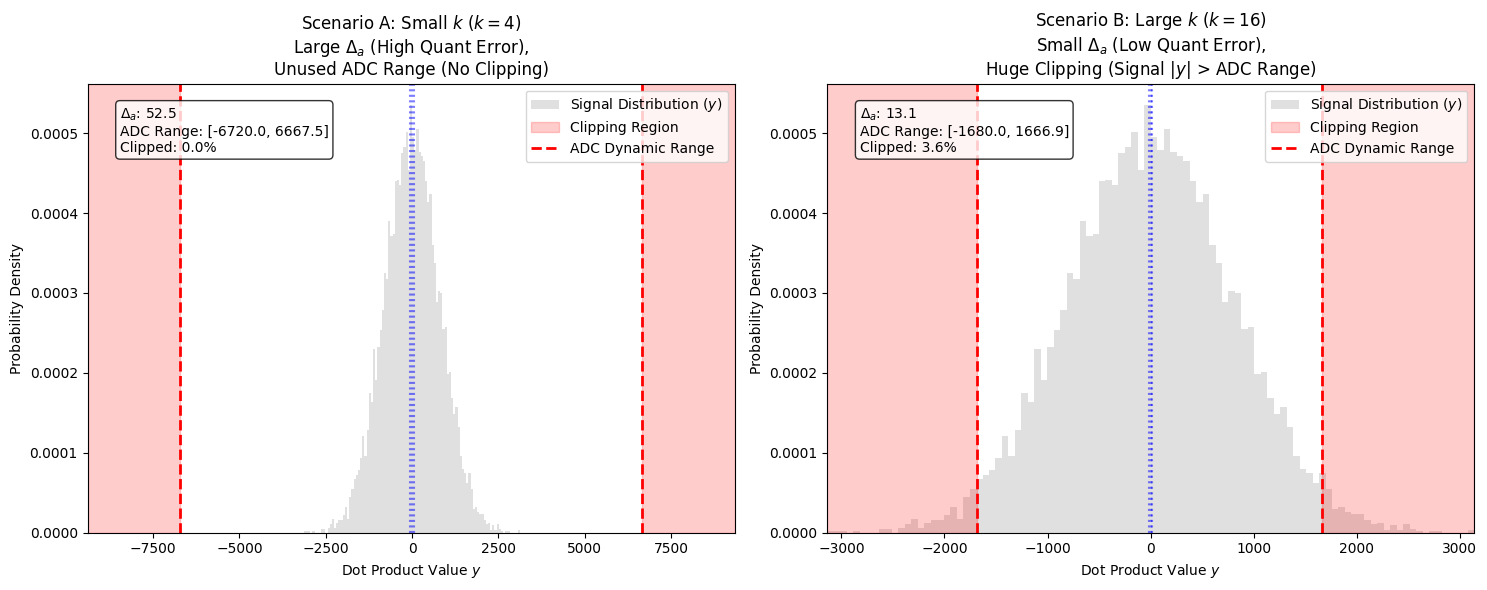
\includegraphics[width=0.7\linewidth]{dead_zone.png}
  \caption{ADC dead-zone illustration. Pre-ADC values in
    $[0,\Delta)$ floor to the zero code, discarding the analog signal
    entirely. The two failure modes (dead zone and clipping) are
    determined by the fixed step $\Delta$ and the $b_a$-bit ADC
    range.}
  \label{fig:dead_zone}
\end{figure}

\begin{figure}[htbp]
  \centering
  \resizebox{0.85\linewidth}{!}{%
  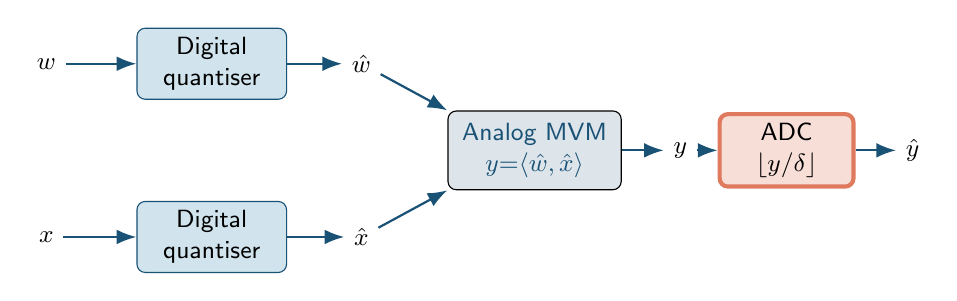
\begin{tikzpicture}[
      every node/.style={font=\small},
      q/.style={draw=mybluedark, rounded corners=3pt, fill=myblue!22,
                minimum width=1.9cm, minimum height=0.72cm, align=center},
      tile/.style={draw, rounded corners=3pt, fill=mybluedark!15, text=mybluedark,
                   minimum width=2.2cm, minimum height=1.0cm, align=center},
      adc/.style={draw=myorange, line width=1.5pt, rounded corners=3pt,
                  fill=myorange!25, minimum width=1.7cm, minimum height=0.72cm,
                  align=center},
      arr/.style={-{Latex[length=2.5mm]}, thick, mybluedark}
    ]
    \node (w)  at (0,   1.1) {$w$};
    \node[q] (qw) at (2.1,  1.1) {Digital\\quantiser};
    \node (wb) at (4.0,  1.1) {$\hat w$};

    \node (x)  at (0,  -1.1) {$x$};
    \node[q] (qx) at (2.1, -1.1) {Digital\\quantiser};
    \node (xb) at (4.0, -1.1) {$\hat x$};

    \draw[arr] (w)--(qw);   \draw[arr] (qw)--(wb);
    \draw[arr] (x)--(qx);   \draw[arr] (qx)--(xb);

    \node[tile] (T) at (6.2, 0) {Analog MVM\\$y{=}\langle\hat w,\hat x\rangle$};
    \draw[arr] (wb) -- (T.north west);
    \draw[arr] (xb) -- (T.south west);

    \node (y)  at (8.05, 0) {$y$};
    \draw[arr] (T)--(y);

    \node[adc] (A) at (9.4, 0) {ADC\\$\lfloor y/\delta\rfloor$};
    \draw[arr] (y)--(A);

    \node (yb) at (11.0, 0) {$\hat y$};
    \draw[arr] (A)--(yb);
  \end{tikzpicture}}
  \caption{Math model of an analog linear layer. Activations $x$ and
    weights $w$ are first quantized digitally to $\hat{x}$ and
    $\hat{w}$. The analog MVM engine then computes the inner product
    $y = \langle \hat{w}, \hat{x} \rangle$ in continuous-valued form.
    Finally the ADC maps $y$ to a discrete output $\hat{y}$ via
    $\lfloor y / \delta \rfloor$, with step size $\delta$ fixed by the
    hardware. The two distinct quantization stages
    (digital input, analog-to-digital output) are formalised in
    Eqs.~\eqref{eq:adc_quantizer}--\eqref{eq:adc_delta_background}.}
  \label{fig:analog_mvm_pipeline}
\end{figure}

The ADC quantizer described above is qualitatively different from the
quantization stages on the digital side of the pipeline. In purely
digital low-bit inference, the dominant errors come from the input
and weight quantizers and from approximate integer arithmetic, and
all of them can be tightened by better calibration. The ADC step
$\Delta$, by contrast, is fixed at manufacturing time and cannot be
reduced by retraining; even if $Q_x$ and $Q_w$ are well calibrated,
the accumulated output can still be projected onto an insufficiently
fine ADC lattice~\cite{RAOQ2024,Buechel2025AnalogFoundation}. The
main bottleneck may therefore shift from input-side quantization to
output quantization, and this distinction is central to the present
thesis.

The problem becomes more severe for transformer models. Their hidden
states are high-dimensional, anisotropic, and may contain rare channels
with extremely large magnitude. These outliers stress the activation
quantizer before the analog array and also distort the distribution of
$y_{\mathrm{int}}$ presented to the ADC. Consequently, the question is
how to quantize weights and activations and how to shape
internal signals so that the analog accumulation uses the ADC range
efficiently \cite{RAOQ2024,Buechel2025AnalogFoundation}.

\subsection{Quantization of Neural Networks}
\label{subsec:quantization_basics}

Large neural networks, and large language models in particular, are
bottlenecked by memory bandwidth and the arithmetic throughput of dense
linear layers in floating-point precision. Quantization addresses this
by representing weights and activations as low-bit integers, trading
numerical accuracy for substantial reductions in model size and compute
cost. In analog or IMC settings this is more than an optimization: the
hardware itself operates at a fixed and often low precision, so the
digital side of the pipeline must match it.

Quantization maps continuous tensors to a finite set of discrete values
in order to reduce memory, bandwidth, and arithmetic cost
\cite{Jacob2018IntegerOnly,Wu2020IntegerQuant,Gholami2021Survey}. In
symmetric uniform quantization, a scalar $x \in \mathbb{R}$ is mapped to
\begin{equation}
q(x)
=
\mathrm{clip}
\!\left(
\left\lfloor \frac{x}{s} \right\rceil,
-q_{\max}, q_{\max}
\right),
\qquad
\hat{x} = s\,q(x),
\label{eq:symmetric_quant_background}
\end{equation}
where $s>0$ is the quantization scale and $q_{\max}=2^{b-1}-1$ for a
signed $b$-bit quantizer. Symmetric quantization is widely used for
weights and signed activations because it preserves zero exactly and
simplifies integer arithmetic.

In asymmetric quantization, one adds a zero-point $z$:
\begin{equation}
q(x)
=
\mathrm{clip}
\!\left(
\left\lfloor \frac{x}{s} + z \right\rceil,
q_{\min}, q_{\max}
\right),
\qquad
\hat{x}
=
s\,(q(x)-z).
\label{eq:asymmetric_quant_background}
\end{equation}
This is useful when the signal distribution is non-negative or strongly
shifted, as in some post-activation tensors or hardware-aware activation
coding schemes \cite{Jacob2018IntegerOnly,Wu2020IntegerQuant}.

Quantization also differs in granularity. In per-tensor
quantization, one scale is shared by the full tensor. In
per-channel quantization, each output channel receives its own
scale; this is particularly useful for weights because different rows of
$W$ often have very different ranges. For transformer activations, one
also encounters per-token and per-group scaling, especially when the
activation distribution changes strongly across tokens or heads.

Two training regimes dominate the literature. In
post-training quantization (PTQ), a pretrained floating-point
model is quantized after training, usually using a small calibration set
and a local reconstruction objective
\cite{ZeroQuant2022,AWQ2023,OmniQuant2023,CBQ2023,FlatQuant2024,QEP2025}.
A generic PTQ objective for layer $\ell$ can be written as
\begin{equation}
\min_{\theta_\ell^q}
\sum_{x \in \mathcal{C}}
\left\|
f_\ell(x;\theta_\ell)
-
\hat{f}_\ell(x;\theta_\ell^q)
\right\|_2^2,
\label{eq:ptq_objective_background}
\end{equation}
where $\mathcal{C}$ is a calibration set and $\theta_\ell^q$ are the
quantized parameters or auxiliary calibration variables. PTQ is
attractive because it avoids retraining the full model.

In quantization-aware training (QAT), quantization is inserted
into the forward pass during training or finetuning:
\begin{equation}
\min_{\theta}
\sum_{(x,y)}
\mathcal{L}
\!\left(
y,\,
f_q(x;\theta)
\right),
\label{eq:qat_objective_background}
\end{equation}
so that the parameters adapt directly to quantization noise
\cite{PACT2018,LSQ2019,LLMQAT2023,EfficientQAT2024}. Since rounding is
non-differentiable, QAT commonly relies on the straight-through
estimator (STE), which uses the quantized function in the forward pass
but approximates its gradient in the backward pass by
\begin{equation}
\frac{\partial q(x)}{\partial x} \approx 1.
\label{eq:ste_background}
\end{equation}
Although heuristic, STE is one of the standard tools behind low-bit QAT
and learned PTQ methods \cite{PACT2018,LSQ2019}.

Several refinements are especially relevant for the present work. PACT
learns activation clipping thresholds \cite{PACT2018}; LSQ learns the
step size itself \cite{LSQ2019}; AdaRound learns non-trivial rounding
decisions in PTQ \cite{AdaRound2020}; and QDrop introduces stochastic
activation dequantization during calibration to stabilize extremely
low-bit PTQ \cite{QDrop2022}. These techniques all point to the same
theme: in low-bit settings, choosing the bitwidth is not enough; one
must also decide how the signal is clipped, scaled, rounded, and
propagated.

\subsection{Challenges of Quantizing Transformer Models}
\label{subsec:transformer_quantization_challenges}

Transformer language models are difficult to quantize. A major reason
is the presence of activation outliers. Dettmers et al.\ introduced
LLM.int8()~\cite{LLMint82022}, the first work to show that hidden
states in transformers contain rare but very large feature values, and
that preserving these outlier dimensions matters even when the rest of
the model is quantized aggressively. The same phenomenon motivates
later methods such as SmoothQuant, Outlier Suppression+, QuaRot,
SpinQuant, and FlatQuant
\cite{SmoothQuant2022,OutlierSuppressionPlus2023,QuaRot2024,SpinQuant2024,FlatQuant2024}.

\begin{figure}[htbp]
  \centering
  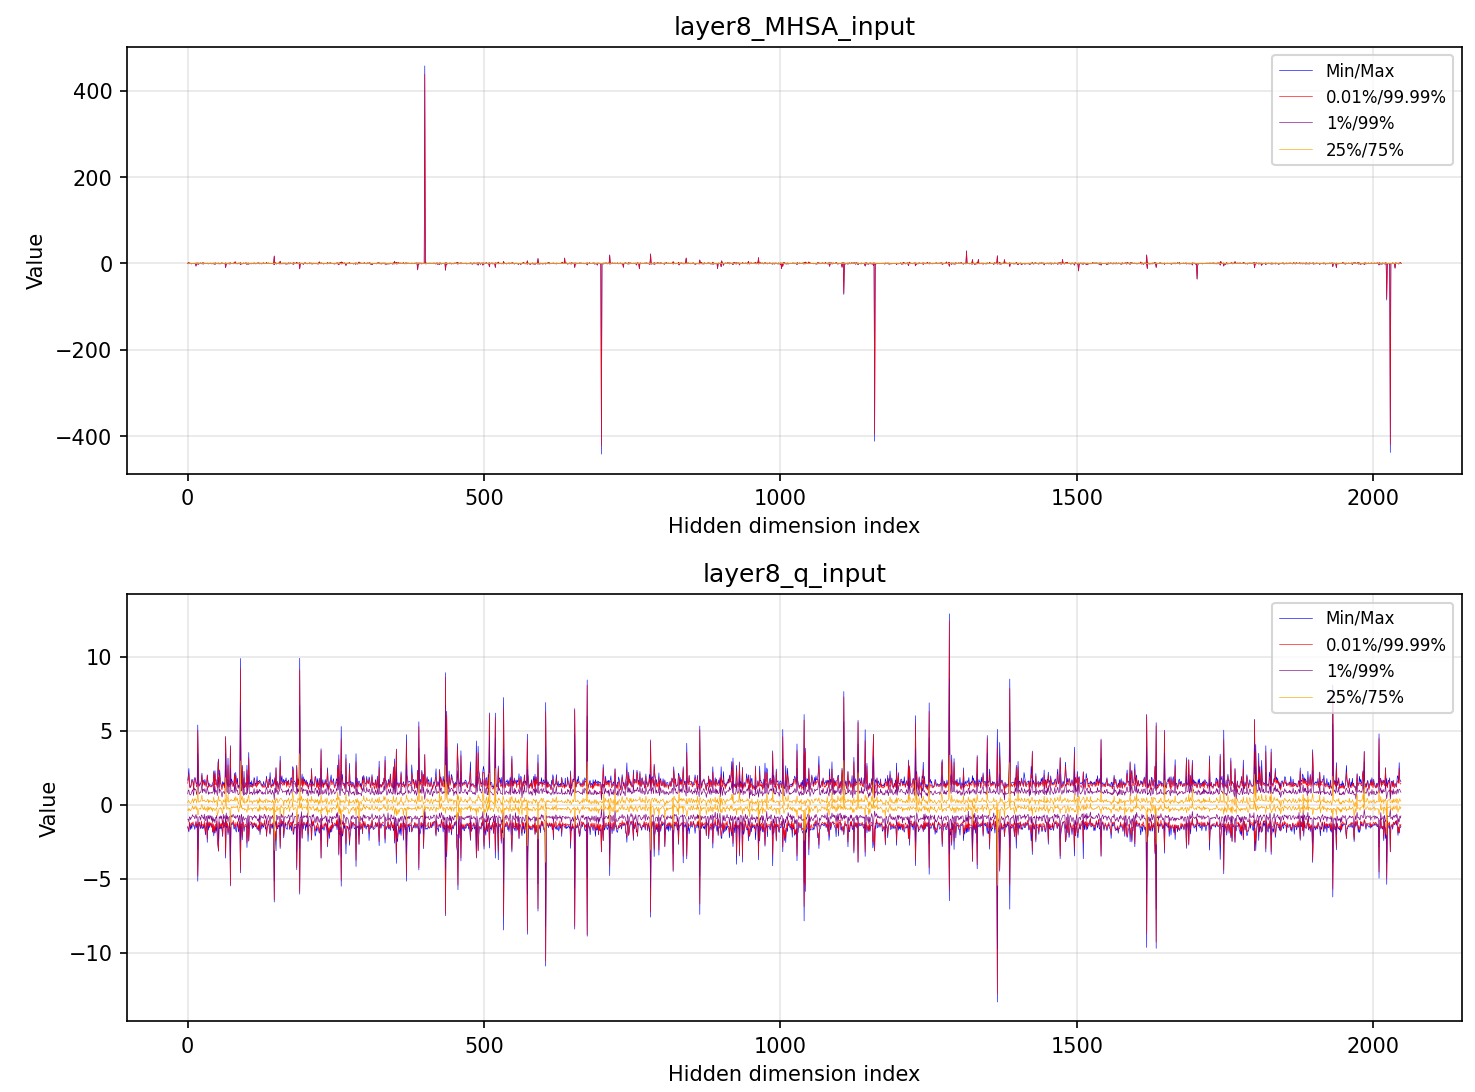
\includegraphics[width=0.78\linewidth]{outliers_layer8.png}
  \caption{Per-channel activation statistics from a single Llama-3.2-1B
    decoder block (layer~8), measured over the WikiText-2 calibration
    set. \emph{Top}: the input to the multi-head self-attention
    sub-layer (\texttt{MHSA input}, i.e.\ the post-RMSNorm hidden
    state). A single hidden dimension reaches values on the order of
    $\pm 400$, while the bulk of channels stays within $\pm 10$.
    \emph{Bottom}: the input to the query projection
    (\texttt{q\_input}) shows the same channel structure compressed
    into a $\pm 10$ range. The colored bands report min/max,
    $0.01$/$99.99$\,\%, $1$/$99$\,\%, and $25$/$75$\,\% percentiles
    across the calibration tokens. Under max-based per-token scaling
    (Eq.~\eqref{eq:per_token_max_scale}), a single such outlier channel
    dominates the scale and forces typical activations into a narrow
    range of integer codes, which is the underlying cause of dead-zone
    behaviour in the downstream ADC.}
  \label{fig:activation_outliers}
\end{figure}

Figure~\ref{fig:activation_outliers} illustrates this on a single
decoder block of Llama-3.2-1B: one hidden dimension carries values two
orders of magnitude larger than the rest.

This is especially problematic under max-based per-token scaling. For a
signed activation tensor, a common choice is
\begin{equation}
s_x
=
\frac{\|x\|_\infty}{q_{\max}},
\label{eq:per_token_max_scale}
\end{equation}
which ensures that the largest feature maps to the largest available
code. If one channel has magnitude $M$ and the remaining channels are of
order $\varepsilon \ll M$, then most quantization levels are allocated
to that single channel. In low-bit settings, many of the smaller
features are then quantized to zero or to a very narrow code band. In an
ADC-constrained pipeline, this not only harms the input code density,
but also leads to poorly occupied output bins after analog accumulation.

A second challenge is the sensitivity of the residual stream. Residual
connections propagate local errors across many layers, so local
reconstruction loss is not always predictive of end-to-end perplexity.
QuaRot explicitly motivates its method by the need to remove outliers
from the residual stream \cite{QuaRot2024}, and SpinQuant shows that
choosing or learning a suitable rotation can dramatically change the
accuracy of low-bit LLM inference \cite{SpinQuant2024}. QEP later argues
that one of the central failures of standard layer-wise PTQ is the
accumulation of quantization errors across layers, and proposes explicit
quantization-error propagation to mitigate this effect
\cite{QEP2025}. CBQ reaches a related conclusion from a cross-block
reconstruction perspective \cite{CBQ2023}.

A third challenge is architectural non-uniformity. Not all transformer
projections are equally sensitive. The output projections
\texttt{o\_proj} and \texttt{down\_proj} inject their errors directly
into the residual stream, whereas earlier projections such as
\texttt{q\_proj}, \texttt{k\_proj}, \texttt{v\_proj},
\texttt{up\_proj}, and \texttt{gate\_proj} are followed by additional
mixing or nonlinear structure before their effect reaches the next
block. This asymmetry is one reason why output-side projections often
emerge as the most sensitive modules in low-bit transformer inference.

Finally, preserving hidden-state geometry is critical. A transform that
reduces scalar range at the price of severely distorting the hidden-state
subspace may still harm model quality. Rotation- and affine-transform
methods are therefore attractive because they attempt to make the model
more quantizable while preserving the underlying full-precision linear
map. This point is especially relevant in the present thesis, where the
goal is to shape the signal path so
that it tolerates both ordinary low-bit quantization and ADC
quantization at the output of each analog MVM, beyond simply reducing local error.

\subsection{Existing Methods}
\label{subsec:existing_methods}

Research on low-bit PTQ for LLMs has converged around a small number
of recurring ideas described in what follows. Two of these methods,
FlatQuant and RAOQ, are central to this thesis and receive extended
treatment.

The earliest line of work reshapes the distribution of activations
before quantisation. SmoothQuant~\cite{SmoothQuant2022} introduces the
diagonal equivalent transformation, which absorbs a per-channel
diagonal $D$ into the weights so that the linear map is preserved:
\begin{equation}
y \;=\; (x D^{-1})\,(D W)^{\top} \;=\; x W^{\top}.
\label{eq:smoothquant_equivalence}
\end{equation}
With $D$ chosen from activation and weight statistics, the rescaled
activation $\tilde x = x D^{-1}$ has reduced peak magnitude, so
per-token max-based scaling no longer collapses around a single
outlier channel. Outlier Suppression+~\cite{OutlierSuppressionPlus2023}
extends this scheme with a per-channel shift that handles asymmetric
outliers; AWQ~\cite{AWQ2023} uses activation statistics to identify
and protect a small set of salient weights; and
OmniQuant~\cite{OmniQuant2023} makes both the diagonal transformation
(LET) and a weight-clipping range (LWC) end-to-end learnable, pushing
PTQ to very low-bit settings such as W4A4.

These methods reshape the activation distribution but leave the
calibration objective itself unchanged. A separate line of work
targets that objective directly, treating PTQ as a calibration problem
in which the quantisation parameters are fit by minimising
reconstruction error against a full-precision reference.
ZeroQuant~\cite{ZeroQuant2022} pairs layer-wise distillation with
hardware-oriented deployment. CBQ~\cite{CBQ2023} generalises the
single-layer objective to cross-block reconstruction, exposing the
optimiser to several consecutive transformer blocks at once.
QEP~\cite{QEP2025} feeds quantised hidden states forward during
calibration, so that the optimisation target reflects accumulated
quantisation error rather than clean teacher activations.

The next line of methods replaces the diagonal scaling of SmoothQuant
with a denser linear transformation. QuaRot~\cite{QuaRot2024} inserts
a fixed Hadamard rotation into the residual stream, removing
large-magnitude directions before quantisation.
SpinQuant~\cite{SpinQuant2024} learns this rotation rather than
drawing it at random, showing that the choice of rotation
substantially affects low-bit accuracy. Both methods act at the level
of the residual stream rather than at the level of individual
projections.

FlatQuant~\cite{FlatQuant2024}, the calibration backbone of this
thesis, sharpens this idea by applying a separate invertible linear
transform to each linear projection of the model:
\begin{equation}
y \;=\; x\,W^{\top}
   \;=\; (x\,T^{-1})\,(T\,W^{\top})
   \;=\; \tilde x\, \tilde W^{\top}.
\label{eq:flatquant_invariance}
\end{equation}
Unlike QuaRot and SpinQuant, the transform $T$ is learned end-to-end
through block-level reconstruction, so every projection has its own
tailored transform that flattens the local activation distribution.
To keep the per-projection parameter count tractable, the
$d \times d$ transform is parameterised as a Kronecker product
\begin{equation}
T \;=\; T_1 \otimes T_2,
\qquad
T_1 \in \mathbb{R}^{a \times a}, \quad
T_2 \in \mathbb{R}^{b \times b}, \quad
ab = d,
\label{eq:flatquant_kron}
\end{equation}
reducing the parameter count from $\mathcal{O}(d^2)$ to
$\mathcal{O}(d)$. After calibration, $T$ is folded into the
surrounding weights, so the inference path is unchanged. At W4A4,
FlatQuant set the strongest published PTQ result on Llama-3 at the
time of writing.

The methods discussed so far operate entirely in the digital domain.
RAOQ~\cite{RAOQ2024} is the first to make the analog-to-digital
boundary itself an object of optimisation. Unlike the PTQ methods
above, RAOQ is a quantisation-aware training (QAT) method: it starts
from a pre-trained model and fine-tunes weights and activations
end-to-end with the ADC included in the forward pass, targeting the
variance of the pre-ADC accumulation $\mathrm{Var}[Y]$, which sets the
signal-to-quantisation-noise ratio of the analog readout. Activation
shifting (A-shift) re-quantises signed activations as unsigned and
shifts them by a constant $C = 2^{b_x-1}$,
\begin{equation}
x_s \;=\; \mathrm{clip}\!\left(\left\lfloor\frac{x-\beta}{s_x}\right\rceil,\,0,\,2^{b_x}-1\right) - C,
\label{eq:raoq_ashift}
\end{equation}
which concentrates the mass of $x_s$ at large absolute values and
increases $\mathbb{E}[X^2]$ by roughly $15\times$ compared with direct
signed quantisation; the resulting offset $C\sum_i w_i$ in the IMC
computation is precomputed offline and adds no inference overhead.
Weight reshaping (W-reshape) adds a kurtosis penalty to the QAT loss
to flatten the weight distribution and increase $\mathrm{Var}[W]$:
\begin{equation}
\kappa \;=\; \mathbb{E}\!\left[\left(\frac{W - \mu_W}{\sigma_W}\right)^{\!4}\right],
\qquad
L_Q \;=\; L_c + \lambda_\kappa \sum_\ell \kappa_\ell,
\label{eq:raoq_kurt}
\end{equation}
with $\mu_W, \sigma_W$ the mean and standard deviation of the weight
tensor and $L_c$ the task loss. Bit augmentation (BitAug) trains the
model under multiple ADC bit precisions simultaneously,
\begin{equation}
L_A \;=\; L(\theta, b_a) + \lambda_b\, L(\theta, \tilde b_a),
\label{eq:raoq_bitaug}
\end{equation}
with $\tilde b_a$ sampled at each iteration from a neighbourhood of
the target bit width; the extra gradients smooth the ADC-induced loss
surface and reduce the chance of getting stuck in local minima. For
models with more than $\sim$200M parameters, RAOQ also fits a
LoRA-style adapter (ADC-LoRA) inside the quantised weight,
$W + AB$, to reduce the gradient-accumulation cost of BitAug; because
$AB$ is summed into the weight before the ADC, this is a pre-ADC
LoRA. Analog Foundation Models~\cite{Buechel2025AnalogFoundation}
take a different position within the same QAT-style family: rather
than tuning a small set of parameters, the entire LLM is fine-tuned
under explicit analog noise constraints, trading training cost for
stronger end-to-end accuracy.

When pure PTQ saturates, a natural next step is to freeze the
quantised backbone and attach a small trainable correction.
LLM-QAT~\cite{LLMQAT2023} applies quantisation-aware training to
extremely low-bit transformers, and
EfficientQAT~\cite{EfficientQAT2024} reduces the cost of this idea
through block-wise parameter updates and end-to-end training of the
quantisation parameters. A related sub-line treats the correction as
low-rank: INT2.1~\cite{INT21_2023}, LQER~\cite{LQER2024}, Low-Rank
Correction for Quantized LLMs~\cite{LowRankCorrection2024}, and
LR-QAT~\cite{LRQAT2024} all show that much of the residual
quantisation error can be captured by training a small low-rank
addition to each linear layer.

\subsection{Research Gap}
\label{subsec:research_gap}

The literature reviewed above establishes two complementary facts.
First, state-of-the-art PTQ methods for LLMs --- scaling-, rotation-,
and reconstruction-based alike --- are highly effective at reducing
input-side activation and weight quantization
error~\cite{SmoothQuant2022, AWQ2023, OmniQuant2023, QuaRot2024,
SpinQuant2024, FlatQuant2024}.  Second, IMC-oriented work shows that
analog output quantization introduces a separate and often dominant
bottleneck that is not naturally captured by ordinary digital PTQ
objectives~\cite{RAOQ2024, Buechel2025AnalogFoundation}.

This creates a specific gap for ADC-constrained LLM inference. Standard
PTQ methods typically optimize a local reconstruction objective
\begin{equation}
\mathcal{L}_{\mathrm{PTQ}}
=
\sum_{x \in \mathcal{C}}
\left\|
f_\ell(x) - \hat{f}_\ell(x)
\right\|_2^2,
\label{eq:standard_ptq_gap}
\end{equation}
possibly with clipping or affine preconditioning. Even when
quantization-error propagation is included, the target is usually still a
digital hidden-state reconstruction objective \cite{QEP2025}. In an IMC
accelerator, however, the effective layer map is
\begin{equation}
\hat{f}^{\mathrm{ADC}}_\ell(x)
=
D_{\mathrm{out}}
\,
Q_{\mathrm{ADC}}
\!\left(
Q_w(W_\ell)\,Q_x(x)
\right),
\label{eq:adc_layer_gap}
\end{equation}
so the model is constrained not only by low-bit inputs and weights, but
also by the ADC quantization of the analog accumulation. Consequently, a
method can achieve strong ordinary PTQ metrics and still perform poorly
once the ADC is inserted into the inference loop.

ADC-aware QAT methods such as RAOQ~\cite{RAOQ2024} and Analog Foundation
Models~\cite{Buechel2025AnalogFoundation} have shown that this output-side
bottleneck can in principle be closed by fine-tuning the entire network
end-to-end with the ADC in the loop. The cost of this approach scales
poorly with model size: full QAT on a billion-parameter LLM requires
hours to days of GPU time per configuration, full-precision gradients
through every quantised layer, and additional memory for techniques like
BitAug that accumulate gradients across several ADC bit widths. ADC-aware
QAT has therefore been demonstrated mostly on convolutional models and on
language models in the 100M--1B range, and does not yet scale comfortably
to the contemporary LLM regime. The first question raised by this gap is
whether transform-based PTQ, which is much cheaper than full QAT, can be
extended to be ADC-aware while retaining model quality.

A second gap appears after pure PTQ saturates. Once the best
transform-based ADC-aware PTQ solution has been found, the remaining
error may no longer be well addressed by additional clipping, scaling,
or rotation heuristics. At that point, the relevant question is whether
the frozen ADC path can be corrected by a lightweight residual branch
rather than by retraining the full model. Although low-rank correction
has been studied in digital low-bit settings
\cite{LQER2024,LowRankCorrection2024,LRQAT2024}, its interpretation as a
post-ADC residual correction on top of a frozen IMC signal path is
not standard in the LLM PTQ literature.

The research gap of this thesis is therefore twofold:
\begin{enumerate}
    \item existing PTQ methods mainly optimize input-side quantization
    error, while ADC-constrained inference introduces a distinct output
    quantization bottleneck that must be modeled explicitly;
    \item once transform-based PTQ saturates, a lightweight residual
    correction stage may be required, but it is unclear where such a
    correction should be inserted and how it should be trained.
\end{enumerate}

The following chapters address these gaps in two stages. First, they
extend transform-based PTQ with ADC-aware objectives, error propagation,
and bounded equivalent scaling. Second, they investigate low-rank
residual correction on top of the frozen quantized ADC path, showing
that post-ADC correction can recover a large fraction of the remaining
accuracy loss in low-bit LLaMA inference.



\section{Problem Statement and Research Questions}
\label{sec:problem_statement}

\subsection{Problem Definition}
\label{subsec:problem_definition}

The core problem studied in this thesis is how to deploy a
transformer LLM on an in-memory computing (IMC) inference path in
which every large linear projection is constrained both by low-bit
weight and activation quantization and by a finite-resolution
analog-to-digital converter (ADC) after the matrix--vector
multiplication.  In a standard digital setting, a linear projection
in a transformer block computes
\begin{equation}
    y = x W^\top + b,
\end{equation}
where \(x \in \mathbb{R}^{d_{\mathrm{in}}}\) is the input hidden state, \(W \in \mathbb{R}^{d_{\mathrm{out}} \times d_{\mathrm{in}}}\) is the projection matrix, and \(b\) is an optional bias term. In the IMC setting considered here, the same operation is executed tile by tile in quantized code space.

Let the input dimension be split into tiles of width \(M\). For tile \(t\), the activation and weight tensors are quantized as
\begin{equation}
    x_t \approx s_{x,t} \hat{x}_t, 
    \qquad
    W_t \approx \operatorname{diag}(\mathbf{s}_{w,t}) \hat{W}_t,
\end{equation}
where \(\hat{x}_t\) and \(\hat{W}_t\) are integer activation and weight codes, \(s_{x,t}\) is the activation scale, and \(\mathbf{s}_{w,t}\) is the vector of per-output-channel weight scales. The analog array accumulates the integer dot product
\begin{equation}
    z_t = \hat{x}_t \hat{W}_t^\top .
\end{equation}
Unlike conventional digital quantization, this accumulated value is not immediately available at full integer precision. It must first be discretized by the ADC:
\begin{equation}
    Q_{\mathrm{ADC}}(z_t; \Delta, n_a, p_a)
    =
    \Delta \cdot
    \operatorname{clip}
    \left(
        \left\lfloor \frac{z_t}{\Delta} \right\rfloor,
        n_a,
        p_a
    \right),
\end{equation}
where \(\Delta\) is the ADC step size and \((n_a,p_a)\) are the lower and upper ADC code bounds. The dequantized output of the tiled projection is then
\begin{equation}
    \hat{y}
    =
    b
    +
    \sum_t
    s_{x,t}
    \left(
        \mathbf{s}_{w,t}
        \odot
        Q_{\mathrm{ADC}}(z_t; \Delta, n_a, p_a)
    \right),
\end{equation}
where \(\odot\) denotes element-wise multiplication.

The ADC step size is a hardware-defined quantity. For the Signed readout used in the main experiments, it is given by
\begin{equation}
    \Delta
    =
    \frac{2 M q_x q_w}{2^{b_a} k},
\end{equation}
where \(b_a\) is the ADC bit-width, \(k\) is the ADC scaling factor, and \(q_x\), \(q_w\) are the maximum activation and weight code levels determined by the activation and weight precisions \(b_x\) and \(b_w\). For the Unsigned shift-subtract readout, the corresponding unsigned step size is
\begin{equation}
    \Delta_u
    =
    \frac{M(2^{b_x}-1)(2^{b_w}-1)}{(2^{b_a}-1)\,k}.
\end{equation}
In both cases, the essential property is the same: the output lattice is fixed by hardware parameters and cannot be made finer by ordinary post-training calibration.

This makes ADC-constrained inference fundamentally different from standard digital post-training quantization (PTQ). A PTQ method may successfully reduce the error in \(\hat{x}_t\) and \(\hat{W}_t\), while the accumulated output \(z_t\) may still be mapped to a coarse ADC lattice. If \(0 \le z_t < \Delta\), the output maps to the zero ADC code under floor quantization; small negative values instead map to the $-1$ code, so the dead-zone rate is measured directly as the fraction of post-ADC codes equal to zero. If \(z_t\) exceeds the ADC range, the output is clipped. Therefore, the objective is to quantize weights and activations accurately and to shape the internal integer accumulation so that the ADC range is used effectively.

The software-side degrees of freedom considered in this thesis are transform-based PTQ parameters and, in the second stage, a lightweight residual adaptation branch. Following the FlatQuant idea, an invertible transform \(T_\ell\) can be inserted into a linear projection without changing the full-precision computation:
\begin{equation}
    x W_\ell^\top
    =
    (x T_\ell^{-1})(T_\ell W_\ell^\top).
\end{equation}
However, after quantization and ADC discretization, this equivalence no longer holds exactly. The practical calibration problem is therefore to choose transforms that minimize the mismatch between the full-precision block output and the ADC-constrained quantized block output:
\begin{equation}
    \min_{\phi}
    \;
    \mathbb{E}_{x \in \mathcal{C}}
    \left[
        \left\|
            B_\ell(x)
            -
            \hat{B}^{\mathrm{ADC}}_\ell(x; \phi, \mathcal{H})
        \right\|_2^2
    \right],
\end{equation}
where \(B_\ell\) is the full-precision transformer block, \(\hat{B}^{\mathrm{ADC}}_\ell\) is its quantized ADC-constrained counterpart, \(\phi\) denotes the PTQ calibration parameters, \(\mathcal{C}\) is the calibration set, and
\begin{equation}
    \mathcal{H} = (b_x, b_w, b_a, M, k, \mathrm{ADC\ mode})
\end{equation}
is the fixed hardware configuration.

At the model level, the goal is to obtain an ADC-constrained model \(\hat{F}^{\mathrm{ADC}}\) whose quality remains close to the full-precision model \(F\) and to the corresponding digital quantized model with the ADC disabled:
\begin{equation}
    \min_{\phi, \psi}
    \;
    \operatorname{PPL}
    \left(
        \hat{F}^{\mathrm{ADC}}_{\phi,\psi};
        \mathcal{D}_{\mathrm{eval}}
    \right),
    \qquad
    \text{subject to fixed } \mathcal{H}
    \text{ and } |\psi| \ll |\theta|.
\end{equation}
Here \(\psi = 0\) corresponds to pure PTQ, while \(\psi\) denotes the optional lightweight residual correction parameters used in the adaptation stage. The central question is whether ADC-aware PTQ alone is sufficient, or whether the fixed ADC output lattice creates a residual error that must be corrected by a small trainable module.

\subsection{Research Questions}
\label{subsec:research_questions}

This thesis is guided by the following research questions.

\begin{description}
    \item[RQ1.]
    \textbf{How much quality degradation is caused specifically by ADC output quantization in LLMs?}

    This question separates ordinary digital quantization error from the additional degradation introduced by the ADC. The comparison is made between full-precision inference, quantized inference with the ADC disabled, and quantized inference with the full ADC path enabled. The goal is to determine whether the ADC is a minor implementation detail or a dominant source of error under low-bit IMC inference.

    \item[RQ2.]
    \textbf{To what extent can FlatQuant-style post-training transformations mitigate ADC-induced degradation?}

    This question studies whether learned equivalent transformations can reshape activation and weight distributions so that the integer accumulation uses the ADC range more effectively. In particular, the thesis evaluates block-wise calibration, propagated quantized inputs, mixed full-precision/ADC objectives, trainable diagonal scaling, and staged training.

    \item[RQ3.]
    \textbf{Is reconstruction-only PTQ sufficient under ADC constraints, or are explicitly ADC-aware objectives required?}

    Standard PTQ methods usually minimize reconstruction error under digital quantization assumptions. This thesis investigates whether such objectives remain predictive once the ADC is inserted into the inference path. The question is answered by comparing clean-input reconstruction, ADC-propagated reconstruction, and objectives that explicitly expose the calibration process to ADC noise.

    \item[RQ4.]
    \textbf{Which layers and projection types are most sensitive to ADC quantization?}

    LLaMA decoder blocks contain several linear projections: \(q\), \(k\), \(v\), \(o\), \(\mathrm{gate}\), \(\mathrm{up}\), and \(\mathrm{down}\). These projections do not contribute equally to end-to-end degradation. This question identifies whether ADC sensitivity is concentrated in particular projections, such as output-side attention and MLP projections, or distributed uniformly across the architecture.

    \item[RQ5.]
    \textbf{Under what conditions does ADC-constrained inference require lightweight model adaptation beyond PTQ?}

    If transform-based PTQ reaches a quality plateau, the remaining error may be caused by the finite ADC output resolution rather than by poorly calibrated weights or activations. This question evaluates whether a small post-ADC residual correction branch can close the remaining quality gap while keeping the quantized ADC backbone frozen.
\end{description}

Together, these questions connect three levels of analysis: the hardware-level ADC discretization, the layer-level behavior of quantized transformer projections, and the model-level language modeling quality.

\subsection{Scope and Assumptions}
\label{subsec:scope_assumptions}

The thesis focuses on a decoder-only transformer LLM, with Llama-3.2-1B used as the main experimental target. This model is large enough to exhibit the activation outlier and residual-stream sensitivity typical of modern LLMs, while still being small enough to support extensive ablation studies over quantization precision, ADC settings, calibration strategies, and residual adaptation variants.

The hardware behavior is studied through simulation rather than through measurements on a fabricated IMC chip. The simulator models tiled integer matrix--vector multiplication, per-token activation quantization, per-channel weight quantization, ADC floor quantization, ADC clipping, and dequantization. Two readout settings are considered: \textbf{Signed} and \textbf{Unsigned}. Signed denotes a signed-accumulation readout with a symmetric ADC code range. Unsigned denotes a single-read unsigned shift-subtract readout, where signed INT4 codes are shifted to non-negative codes before the MVM and the zero-point terms are subtracted digitally after ADC readout. The hardware parameters \(M\), \(b_x\), \(b_w\), \(b_a\), and \(k\) are treated as fixed during each experiment unless an explicit per-layer \(k\)-search experiment is performed.

Several hardware effects are outside the scope of this work. The simulator does not model device-to-device variation, thermal noise, conductance drift, IR drop, nonlinear crossbar behavior, write noise, peripheral circuit latency, or full chip-level energy consumption. The purpose of the study is therefore not to claim final hardware efficiency for a specific IMC implementation, but to isolate the algorithmic consequences of ADC output discretization.

The quantization study is restricted to the main linear projections inside the transformer decoder blocks. Other components, such as layer normalization, nonlinearities, softmax, rotary embeddings, and token embeddings, are not the primary target of the ADC simulation. This restriction reflects the fact that large linear projections dominate transformer inference cost and are the most natural mapping target for IMC arrays.

The main methodological focus is post-training quantization. The thesis does not retrain the full model and does not modify the original pretraining objective. When adaptation is considered, it is limited to a small residual low-rank branch trained on top of a frozen quantized ADC path. This allows the thesis to distinguish between what can be achieved by calibration alone and what requires additional trainable parameters.

The calibration data is finite and substantially smaller than the original pretraining data. Therefore, the reported results should be interpreted as evidence about practical calibration and adaptation under limited data, not as an upper bound on what could be achieved with large-scale quantization-aware training.

\subsection{Evaluation Criteria}
\label{subsec:evaluation_criteria}

The primary model-level metric is perplexity. For each configuration, the thesis compares
\begin{equation}
    \operatorname{PPL}_{\mathrm{FP}},
    \qquad
    \operatorname{PPL}_{\mathrm{no\,ADC}},
    \qquad
    \operatorname{PPL}_{\mathrm{ADC}},
\end{equation}
where \(\operatorname{PPL}_{\mathrm{FP}}\) is the full-precision baseline, \(\operatorname{PPL}_{\mathrm{no\,ADC}}\) measures quantized inference with the ADC disabled, and \(\operatorname{PPL}_{\mathrm{ADC}}\) measures the full ADC-constrained inference path. The difference between no-ADC and ADC perplexity isolates the degradation introduced by output quantization:
\begin{equation}
    \Delta_{\mathrm{ADC}}
    =
    \operatorname{PPL}_{\mathrm{ADC}}
    -
    \operatorname{PPL}_{\mathrm{no\,ADC}},
\end{equation}
while the ratio
\begin{equation}
    \rho_{\mathrm{ADC}}
    =
    \frac{
        \operatorname{PPL}_{\mathrm{ADC}}
    }{
        \operatorname{PPL}_{\mathrm{no\,ADC}}
    }
\end{equation}
measures the relative severity of the ADC bottleneck. A successful ADC-aware method should reduce both \(\operatorname{PPL}_{\mathrm{ADC}}\) and the no-ADC-to-ADC gap without severely degrading no-ADC quality.

In addition to perplexity, the thesis uses internal ADC-level metrics to diagnose why a configuration succeeds or fails. The dead-zone rate is defined as the fraction of pre-ADC accumulated values whose post-ADC code is exactly zero,
\begin{equation}
    r_{\mathrm{dead}}
    =
    \frac{1}{N}
    \sum_{i=1}^{N}
    \mathbf{1}
    \left[
        \left\lfloor z_i / \Delta \right\rfloor = 0
    \right],
    \label{eq:dead_rate}
\end{equation}
where \(z_i\) denotes a pre-ADC accumulated value. This is the floor-consistent definition: $\lfloor z_i / \Delta\rfloor = 0$ holds for $z_i \in [0,\Delta)$ in both the Signed and Unsigned readouts. A high dead-zone rate indicates that many analog outputs are too small to register on the ADC lattice. The clipping rate is defined as
\begin{equation}
    r_{\mathrm{clip}}
    =
    \frac{1}{N}
    \sum_{i=1}^{N}
    \mathbf{1}
    \left[
        c_i = n_a
        \;\;\mathrm{or}\;\;
        c_i = p_a
    \right],
\end{equation}
where \(c_i\) is the ADC code after discretization and clipping. This metric detects whether the integer accumulation systematically exceeds the representable ADC range.

The thesis also evaluates ADC bin utilization:
\begin{equation}
    u_{\mathrm{bin}}
    =
    \frac{
        \left|
            \{c_i : i = 1,\ldots,N\}
        \right|
    }{
        2^{b_a}
    },
\end{equation}
which measures how much of the available ADC codebook is actually used. Low bin utilization indicates that the ADC behaves like a much lower-precision device than its nominal bit-width suggests.

Layer-level reconstruction quality is measured by the relative error
\begin{equation}
    e_\ell
    =
    \frac{
        \left\|
            \hat{y}_\ell
            -
            y^\star_\ell
        \right\|_2^2
    }{
        \left\|
            y^\star_\ell
        \right\|_2^2
    },
\end{equation}
where \(y^\star_\ell\) is the full-precision reference output and \(\hat{y}_\ell\) is the quantized ADC output. This metric is used to identify local failures even when the final perplexity alone does not reveal their source.

Architectural sensitivity is studied at the projection level. For a given projection $p$, the per-projection ADC sensitivity is defined as
\begin{equation}
    \Delta^p_{\mathrm{ADC}}
    \;=\;
    \operatorname{PPL}_{\mathrm{ADC}}
    -
    \operatorname{PPL}_{\mathrm{ADC}\,\setminus\,p},
    \label{eq:per_proj_sensitivity}
\end{equation}
where \(\operatorname{PPL}_{\mathrm{ADC}\,\setminus\,p}\) is the perplexity when the ADC is switched off on \(p\) alone, while digital quantisation and the ADC on every other projection remain active. Summing \(\Delta^p_{\mathrm{ADC}}\) over all projections approximately recovers the global \(\Delta_{\mathrm{ADC}}\); the individual values reveal whether the ADC bottleneck is concentrated in a few projections or distributed uniformly across the architecture.

For residual adaptation experiments, three metrics are tracked together. The closing fraction
\begin{equation}
    \eta
    \;=\;
    \frac{
        \operatorname{PPL}^{\mathrm{PTQ}}_{\mathrm{ADC}}
        -
        \operatorname{PPL}^{\mathrm{PTQ{+}LoRA}}_{\mathrm{ADC}}
    }{
        \operatorname{PPL}^{\mathrm{PTQ}}_{\mathrm{ADC}}
        -
        \operatorname{PPL}_{\mathrm{FP}}
    }
    \label{eq:closing_fraction}
\end{equation}
measures how much of the remaining PTQ-to-FP gap is closed by the adaptation. The parameter overhead
\begin{equation}
    \rho_{\mathrm{params}}
    \;=\;
    \frac{
        \sum_\ell (|A_\ell| + |B_\ell|)
    }{
        \sum_\ell |W_\ell|
    }
    \label{eq:param_overhead}
\end{equation}
measures the size of the added correction relative to the base model, where \(A_\ell, B_\ell\) are the low-rank factors at layer \(\ell\). Out-of-domain generalisation is measured by the C4 ADC perplexity of the same LoRA checkpoint without re-calibration. A successful method achieves \(\eta\) close to one with small \(\rho_{\mathrm{params}}\) and a small C4 ADC perplexity gap.


  \section{Proposed Method}\label{sec:method}

  \subsection{Post-Training Quantization}

  \subsubsection{Baseline: FlatQuant for LLaMA}

  As discussed in Sec.~\ref{subsec:existing_methods},
  FlatQuant~\cite{FlatQuant2024} inserts a learnable invertible
  transform $T = T_1 \otimes T_2$ into each linear projection and
  folds it into the surrounding weights after calibration, so the
  deployed inference cost is unchanged.  The Kronecker factor sizes
  are chosen automatically to factor each projection's input
  dimension $d_{\mathrm{in}}$ into a pair of integers
  $(p, q)$ with $p \cdot q = d_{\mathrm{in}}$ and $p \approx q$, so
  that $T_1 \in \mathbb{R}^{p \times p}$,
  $T_2 \in \mathbb{R}^{q \times q}$, and the parameter count grows
  as $\mathcal{O}(p^2 + q^2) = \mathcal{O}(d_{\mathrm{in}})$ rather
  than $\mathcal{O}(d_{\mathrm{in}}^2)$.

  For Llama-3.2-1B (residual width $d = 2048$, FFN intermediate
  width $d_{\mathrm{ffn}} = 8192$) the per-projection factorisations
  are therefore not uniform.  The six projections whose input is the
  residual stream --- $q, k, v$, and $o$ in the grouped-query
  attention sub-layer, and \texttt{gate} and \texttt{up} in the
  SwiGLU feed-forward network --- have $d_{\mathrm{in}} = 2048$ and
  use $32 \times 64$ Kronecker factors.  The remaining projection,
  \texttt{down}, takes the wider FFN activation as input
  ($d_{\mathrm{in}} = 8192$) and uses $64 \times 128$ factors
  accordingly.  All seven projections in each of the $16$ decoder
  blocks are wrapped, for a total of $7 \times 16 = 112$ transforms
  across the model.

  Calibration uses a teacher--student objective computed at the
  transformer-block level. For each block $B$, a frozen full-precision
  teacher produces a reference output $y^\star = B_{\mathrm{FP}}(x^\star)$,
  and the quantised student $\hat{B}_T$ is optimised over the Kronecker
  factors of all seven projections inside the block, with weights kept
  at their quantised values. Gradients therefore propagate through the
  full block sequence
  $q/k/v \to \mathrm{attn} \to o \to \mathrm{gate}/\mathrm{up} \to \mathrm{down}$,
  so the transforms of earlier projections are aware of how their
  error reaches later ones. The ADC quantiser of
  Eq.~\eqref{eq:adc_quantizer} is included in the student's forward
  pass, so calibration sees the same floor and clipping non-linearities
  as deployment. The non-differentiable round and floor operations of
  the weight, activation, and ADC quantisers are handled by the
  straight-through estimator (STE).

  \subsubsection{Cross-Block Propagation}

  The block-level objective of the baseline above uses the clean
  teacher input $x^\star$ at every block,
  \begin{equation}
      \mathcal{L}_{\mathrm{FP}}
      \;=\;
      \bigl\| \hat{B}(x^\star) - B_{\mathrm{FP}}(x^\star) \bigr\|_2^2,
      \label{eq:loss_fp}
  \end{equation}
  whereas at inference each block receives the ADC-quantised output
  of the preceding one. To close this train--deploy mismatch, blocks
  are calibrated sequentially from layer $0$ to layer $N{-}1$. When
  training layer $\ell$, its input is the ADC-quantised output
  produced by the already-trained layer $\ell{-}1$ rather than a
  clean FP activation. The propagated loss
  \begin{equation}
      \mathcal{L}_{\mathrm{ADC}}
      \;=\;
      \bigl\| \hat{B}(\hat{x}) - B_{\mathrm{FP}}(x^\star) \bigr\|_2^2,
      \label{eq:loss_adc}
  \end{equation}
  where $\hat{x}$ is the ADC-quantised input from the previous block,
  matches the training distribution to the deployment distribution.

  Sequential block-by-block calibration is slower than calibrating
  all blocks in parallel, because each block depends on the trained
  transforms of the preceding ones. An alternative route is taken by
  AIMC work that approximates the ADC as additive noise on top of the
  analog accumulation~\cite{Xiao2021AnalogAccuracy,LeGallo2023AnalogNAS,Buechel2025AnalogFoundation}:
  with such a noise model the input to each layer can be sampled
  directly, and every layer can be calibrated in parallel without
  waiting for the preceding ones. This trades the exact floor-and-clip
  ADC model used here for a smoother stochastic surrogate. The present
  thesis keeps the exact ADC model and accepts the sequential cost;
  the noise-based parallelisation is out of scope but is in principle
  compatible with the same set of ADC-aware extensions.

  \subsubsection{$\alpha$-Mixing of the FP and ADC Objectives}

  Training only on $\mathcal{L}_{\mathrm{ADC}}$ makes the gradients
  unstable: the straight-through estimator passes through several
  floor operations, and the Kronecker rotations start to overfit to
  the ADC noise rather than to the underlying signal. The opposite
  also fails: training only on $\mathcal{L}_{\mathrm{FP}}$ keeps the
  gradients clean, but the block never learns to handle the ADC
  distortion it will see at inference. A mixed objective addresses
  both failure modes by interpolating the two losses with a scalar
  $\alpha \in [0,1]$:
  \begin{equation}
      \mathcal{L}(\alpha)
      \;=\;
      (1 - \alpha)\,\mathcal{L}_{\mathrm{FP}}
      + \alpha\,\mathcal{L}_{\mathrm{ADC}}.
      \label{eq:alpha_mix}
  \end{equation}
  Intuitively, $\mathcal{L}_{\mathrm{FP}}$ supplies a stable learning
  signal that anchors the transform to the FP teacher, while
  $\mathcal{L}_{\mathrm{ADC}}$ teaches the block to tolerate the
  discretisation introduced by the ADC. The value $\alpha = 0$
  recovers clean calibration and $\alpha = 1$ is full propagation.

  In the INT8 setting, full propagation alone drops ADC perplexity
  from $28.86$ to $14.55$, and adding a small bin-center regulariser
  further reduces it to $14.41$, so an $\alpha$-sweep is not needed
  because the noise from full propagation is already manageable. In
  the INT4 setting full propagation is too noisy: the $\alpha$-sweep
  in Section~\ref{sec:results} shows that $\alpha = 0.5$ gives the
  best trade-off, with smaller $\alpha$ under-weighting the ADC
  regime and larger $\alpha$ degrading transform quality through
  gradient noise from the heavier quantisation.



  \subsubsection{Bounded FlatQuant Scaling and Placement}
  \label{sec:diagonals}

  The bound established below applies to the orthogonal part of the
  transform and explains why rotation-like transformations alone
  have limited ability to suppress persistent per-channel outliers.
  FlatQuant already includes a learnable per-channel scaling
  vector as part of its affine pre-quantisation
  transformation~\cite{FlatQuant2024}, and the implementation also
  parameterises each Kronecker factor as
  $U\,\mathrm{diag}(s)\,V^{\top}$ (see Sec.~\ref{app:code:kron}),
  so the deployed transform is not purely rotational even before
  the external scaling is added.  In this thesis we use the
  FlatQuant scaling component in the ADC-aware setting and focus
  on three aspects that are not addressed by the original digital
  PTQ formulation: a bounded form for the external per-channel
  scaling, its placement across attention and MLP sub-layers, and
  its staged calibration under ADC-propagated inputs.

  \begin{lemma}[Orthogonal rotation-only outlier suppression bound]
    \label{lem:rotation-bound}
    This lemma analyses the strict rotation-only subfamily of the
    transform, in which the Kronecker factors are orthogonal and any
    internal singular values or external diagonal scalings are fixed
    to one.  Concretely, let $P = L \otimes R$ with
    $L^{\top}L = I$, $R^{\top}R = I$ be an orthogonal Kronecker
    transform on $\mathbb{R}^d$
    ($d = a \cdot b$,
    $L \in \mathbb{R}^{a \times a}$,
    $R \in \mathbb{R}^{b \times b}$),
    and assume no additional diagonal or singular-value scaling is
    applied.  For any $x \in \mathbb{R}^d$ define the effective
    participation ratio
    \[
      m_{\mathrm{eff}}(x) \;=\; \frac{\|x\|_2^2}{\|x\|_\infty^2}
      \;\in\; [1,\, d].
    \]
    Then for every such orthogonal Kronecker transform $P$,
    \[
      \|xP\|_\infty \;\ge\; \frac{\|x\|_2}{\sqrt{d}},
    \]
    and consequently the maximum achievable suppression of the peak
    activation over all such $P$ satisfies
    \[
      \frac{\|x\|_\infty}{\min_{P}\,\|xP\|_\infty}
      \;\le\;
      \sqrt{\frac{d}{m_{\mathrm{eff}}(x)}}.
    \]
  \end{lemma}

  \begin{proof}
    Since $P$ is orthogonal,
    \[
      \|xP\|_2 \;=\; \|x\|_2.
    \]
    For any vector $y \in \mathbb{R}^d$ the standard
    $\ell^\infty$--$\ell^2$ inequality gives
    \[
      \|y\|_\infty \;\ge\; \frac{\|y\|_2}{\sqrt{d}}.
    \]
    Applying this to $y = xP$ yields
    \[
      \|xP\|_\infty
      \;\ge\;
      \frac{\|xP\|_2}{\sqrt{d}}
      \;=\;
      \frac{\|x\|_2}{\sqrt{d}},
    \]
    which is the first claim. The suppression ratio bound then
    follows from the definition
    \[
      \|x\|_\infty \;=\; \frac{\|x\|_2}{\sqrt{m_{\mathrm{eff}}(x)}}
    \]
    combined with the lower bound on $\|xP\|_\infty$ above:
    \[
      \frac{\|x\|_\infty}{\|xP\|_\infty}
      \;\le\;
      \frac{\|x\|_2 / \sqrt{m_{\mathrm{eff}}(x)}}{\|x\|_2 / \sqrt{d}}
      \;=\;
      \sqrt{\frac{d}{m_{\mathrm{eff}}(x)}}.
    \]
  \end{proof}

  The bound above is not a claim about the full implemented FlatQuant
  parameterisation.  In the implementation each Kronecker factor is
  represented as $U_i \,\mathrm{diag}(s_i)\, V_i^{\top}$
  (Sec.~\ref{app:code:kron}), and the external per-channel scaling
  vector $D$ is exposed through the \texttt{diag\_scale} parameter.
  Once either the internal singular values $s_i$ or the external
  diagonal $D$ are learned, the transform is no longer orthogonal
  and Lemma~\ref{lem:rotation-bound} does not directly apply.  The
  internal singular values $s_L, s_R$ do introduce anisotropy, but it
  is Kronecker-separable: the effective singular values of
  $T_L \otimes T_R$ factor as $s^{(L)}_i\,s^{(R)}_j$, giving only
  $a + b$ degrees of freedom, whereas the external per-channel
  diagonal $D$ gives $d = a\,b$ independent channel scales.  The
  lemma is therefore used as a diagnostic for the strict
  rotation-only subcase; the experiments then study how the
  FlatQuant scaling component behaves under ADC-aware calibration.

  \begin{corollary}[Kronecker capacity]
    \label{cor:kronecker-capacity}
    A full orthogonal matrix on $\mathbb{R}^d$ has
    $d(d-1)/2$ free parameters.
    The Kronecker family $L \otimes R$ has only
    $a(a-1)/2 + b(b-1)/2$ free parameters; for $d = 2048 = 32 \times 64$
    this is $2512$ vs.\ $\approx 2.1 \times 10^6$.
    Consequently, the Kronecker family is a strict low-dimensional subset
    of all orthogonal transforms and may not attain the bound in
    Lemma~\ref{lem:rotation-bound}; the true achievable suppression ratio
    can be strictly smaller.
  \end{corollary}

  In the present setting, per-token activation scaling sets
  $s_x = \|x\|_\infty / q_{\max}$.  If a small number of channels
  persistently dominate (i.e.\ $m_{\mathrm{eff}} \ll d$),
  Lemma~\ref{lem:rotation-bound} gives a ceiling on how much any
  purely rotational transform can help.  For $d = 2048$ and 8
  dominant channels ($m_{\mathrm{eff}} \approx 8$), the maximum
  suppression factor is $\sqrt{2048/8} = 16$; when the required
  suppression exceeds this, the orthogonal component of the
  transform alone cannot escape the bound.  The learnable singular
  values inside the Kronecker factors relax this constraint
  somewhat but remain structurally coupled to the Kronecker
  product, so they do not provide direct per-channel control either.
  The activation distributions discussed in
  Section~\ref{subsec:transformer_quantization_challenges} and shown
  in Figure~\ref{fig:activation_outliers} are exactly this regime: a
  single hidden dimension carries values two orders of magnitude
  above the typical scale, so $m_{\mathrm{eff}} \ll d$.  This is
  what the explicit per-channel diagonal is added for.

  The mechanism is geometric. A Kronecker rotation reshapes the
  covariance of an activation cloud but does not adjust per-channel
  scales, and the residual outlier channels that remain after rotation
  (a few channels with magnitudes $5$--$10\times$ the median) force
  the per-token scale factor to waste range on those channels and
  under-represent the rest. This worsens the ADC dead-zone rate
  because $y_{\mathrm{int}}$ per output channel depends on how
  uniformly codes are distributed across the output range.

  We therefore retain the FlatQuant learnable scaling component
  and write the external per-channel part explicitly as
  $D = \mathrm{diag}(d_1, \ldots, d_c)$,
  attached to the rotation as $\tilde{T} = T \cdot D$ and absorbed
  by an equal-and-opposite rescaling of the weights:
  \[
    y \;=\;
      \underbrace{(x\,D^{-1}T^{-1})}_{\tilde{x}}\,
      \underbrace{(T\,D\,W^\top)}_{\tilde{W}^\top}.
  \]
  This diagonal is not claimed as a new equivalent transformation;
  it is the FlatQuant scaling component reused in the ADC-aware
  setting.  Our contribution in this section is its bounded
  form, sub-system placement, and staged training schedule
  (Sec.~\ref{sec:int4_diagonals}).  The bound is enforced as a
  projection step in the optimiser, $d_i \in [10^{-4}, 10]$, which
  prevents degenerate scaling without altering the calibration
  objective.  $D$ is trained jointly with $T$ during block-level
  calibration and folded into $\tilde{W}$ at deployment, so the
  inference cost is unchanged.  Unlike the strict rotation-only
  subfamily analysed in Lemma~\ref{lem:rotation-bound}, $D$
  changes per-channel magnitudes directly and therefore escapes the
  $\ell^2$-energy invariance assumed there: picking $d_j > 1$
  amplifies row $j$ of $\tilde{W}$ (where it is absorbed cleanly by
  per-channel weight scaling) and equivalently shrinks channel $j$
  of the rotated activation $\tilde{x}$ by a factor $1/d_j$.  For
  an outlier activation channel this is exactly the per-channel
  rebalancing that per-token activation scaling cannot perform.

  Separate diagonals are placed before the attention sub-layer
  (one shared by $q/k/v$, plus a second instance before $o$) and
  before the FFN sub-layer (one shared by \texttt{gate} and
  \texttt{up}, plus a second before \texttt{down}).  We refer to
  these two as the \emph{attention diagonal} and the \emph{MLP
  diagonal}.  An ablation (Section~\ref{sec:results}) shows that
  both placements are necessary: the MLP diagonal drives the no-ADC
  perplexity improvement while the attention diagonal closes the
  ADC gap; either alone leaves significant perplexity on the table.

  In the implementation, the external per-channel diagonal $D$
  studied in this section corresponds to the optional
  \texttt{diag\_scale} parameter (gated by the \texttt{add\_diag}
  flag).  The two further parameters \texttt{diag\_left} and
  \texttt{diag\_right} that appear in
  Listing~\ref{lst:kron} are internal singular values of the
  individual Kronecker factors $T_1$ and $T_2$; they are part of the
  SVD-style Kronecker parameterisation and are \emph{not} counted as
  the per-channel diagonal component studied in the placement and
  staging ablations of Section~\ref{sec:int4_diagonals}.

  \subsubsection{Staged Training}\label{sec:staged}

  Training all Kronecker factors and diagonals jointly from scratch
  with $\alpha = 0.5$ is unstable: attention gradients dominate early
  optimization before MLP transforms have converged, yielding a poor
  initialization for both sub-systems.

  Calibration is split into two stages.  In both stages the
  Kronecker factors of all seven projections
  ($q, k, v, o, \texttt{gate}, \texttt{up}, \texttt{down}$) remain
  trainable; the staging acts on the per-channel diagonals
  $D^{(\mathrm{m})}$ and $D^{(\mathrm{a})}$ and on the learning
  rate.  Stage~A (30 epochs, learning rate $\eta$, $\alpha = 0$)
  enables only the MLP diagonals $D^{(\mathrm{m})}$ and freezes the
  attention diagonals $D^{(\mathrm{a})}$; the Kronecker factors are
  optimised throughout under the clean-input reconstruction loss,
  while the MLP scaling converges in a stable, noise-free regime.
  Stage~B (10 epochs, learning rate $0.1\eta$, $\alpha = 0.5$)
  freezes $D^{(\mathrm{m})}$ at its Stage-A value and enables
  $D^{(\mathrm{a})}$; the Kronecker factors continue to be
  optimised but with a $10\times$ lower learning rate, so the MLP
  basis is effectively held in place while the attention diagonal
  is fitted under ADC-propagated inputs.  The warm MLP start
  prevents gradient interference between the two sub-systems.
  
  Among configurations that reach the pure-PTQ INT4 plateau, this procedure attains the best
  no-ADC perplexity, indicating a better-conditioned underlying
  transform.

  \subsection{Quantization-Aware Adaptation via Post-ADC Residual LoRA}

  PTQ methods reach a floor in the high-20s of ADC perplexity for
  INT4 (around 26--28) regardless of calibration strategy.
  The limiting factor is ADC resolution: with $\delta \approx 6.12$
  each output channel has at most $\sim$30 usable discrete levels,
  introducing irreducible rounding error that no linear transform can
  eliminate.
  PTQ is complemented by a lightweight adaptation step that learns to
  correct ADC distortion after it has occurred, in the digital
  domain, without modifying the frozen quantized model.

  % \begin{figure}[htbp]
  %   \centering
  %   
\includegraphics[width=0.65\linewidth]{plot_ptq_plateau.pdf}
  %   \caption{Pure PTQ plateau. After all transform-based PTQ
  %     improvements (sample count, $\alpha$-mixing, diagonals, staged
  %     training), INT4 ADC perplexity saturates around 27.5--28.5,
  %     independent of calibration strategy. The remaining gap to the
  %     FP and INT8 baselines motivates the post-ADC residual
  %     correction stage.}
  %   \label{fig:ptq_plateau}
  % \end{figure}

  \subsubsection{Architecture}

  The PTQ checkpoint is frozen entirely.
  For each of the seven linear projections in every decoder block, a
  parallel low-rank branch is added that reads the full-precision input
  $x_{\mathrm{fp}}$ and adds its output to the ADC result:
  \[
    y = \underbrace{\mathrm{ADC}_{\mathrm{frozen}}(\hat{x})}_{\text{quantized path}}
      + \underbrace{\frac{\alpha_r}{r}\,B\!\left(A\!\left(x_{\mathrm{fp}}\right)\right)}_{\text{residual correction, rank }r},
  \]
  where $A \in \mathbb{R}^{r \times d}$ and $B \in \mathbb{R}^{d \times r}$
  are LoRA~\cite{lora} factors stored and computed in \texttt{float32},
  and $\alpha_r / r$ is the standard LoRA scaling. The default
  configuration uses rank $r = 4$ on all seven projections of every
  decoder block, with $\alpha_r = 8$ (scaling factor $2.0$). All base
  model parameters (weights, Kronecker factors, diagonals, and ADC
  step sizes) remain frozen throughout. The added rank-$4$ adapters
  contribute roughly $0.22\%$ extra parameters relative to the base
  model; the full overhead breakdown across rank and target choices
  is reported alongside the empirical sweep in
  Sec.~\ref{sec:results}.

  \subsubsection{Training Objective}

  The adapters are trained for 5 epochs with learning rate $10^{-4}$
  using AdamW on the same 1024-sample WikiText-2 calibration set used
  by the staged PTQ checkpoint of Sec.~\ref{sec:int4_diagonals}.
  The loss combines cross-entropy on the next-token prediction with a
  knowledge-distillation term toward the FP teacher:
  \[
    \mathcal{L}_{\mathrm{LoRA}} = \mathrm{CE}(\hat{p},\, y)
    + \lambda\,\mathrm{KL}\!\left(\hat{p}_T \;\big\|\; p_{\mathrm{FP},T}\right),
  \]
  with $\lambda = 0.5$ and temperature $T = 2.0$ on both teacher and
  student logits. The FP teacher forward pass is computed once per
  batch with no gradient. Ablations (Section~\ref{sec:results}) show
  that the KL term improves ADC perplexity over CE alone, that rank
  $r = 4$ saturates the gain, and that covering all 16 decoder blocks
  is necessary because ADC distortion accumulates across depth.

  \subsubsection{Why Post-ADC Placement}

  Placing the LoRA correction before the ADC, modifying the
  pre-ADC integer signal, fails to converge.
  Any correction $\Delta = B A x$ is itself quantized by the fixed
  step $\delta$ before reaching the output, so it cannot express
  sub-$\delta$ adjustments.
  Moreover, gradients through the floor operator are too noisy for
  stable training from a cold start, and the coupled interaction with
  the hard ADC clamp causes the training run to diverge.

  Post-ADC placement avoids both problems: the correction is added in
  the digital domain after the ADC read, at full floating-point
  precision, with clean gradients from the CE+KL loss. As a result,
  ADC perplexity drops below the PTQ plateau on WikiText-2 and
  surpasses the deployed INT8 $+$ ADC PTQ checkpoint used in
  Table~\ref{tab:main_results}, not the ideal no-ADC INT8 digital
  baseline.  The same configuration also improves C4 ADC perplexity,
  confirming that the correction generalises beyond the calibration
  domain.

  \section{Experiments and Results}\label{sec:results}\label{sec:experimental_setup}

  \subsection{Model, Data, and Hardware Setup}

  \paragraph{Model.}
  All experiments use Llama-3.2-1B~\cite{llama3} in \texttt{bfloat16}.
  The model has 16 decoder layers, hidden dimension $d = 2048$, 32
  attention heads with grouped-query attention, and a SwiGLU FFN with
  intermediate dimension 8192.
  This model is chosen because it admits extensive calibration and
  ablation experiments within a single-GPU budget while exhibiting
  the architectural features (grouped-query attention, SwiGLU FFN,
  RMSNorm) shared with larger decoder-only transformer LLMs.

  \paragraph{Calibration data.}
  FlatQuant transforms and LoRA adapters are calibrated on WikiText-2
  training text~\cite{wikitext2}.
  Unless stated otherwise, 128 randomly sampled sequences of 2048 tokens
  each are used.
  Selected experiments use 512 or 1024 samples to study the effect of
  calibration set size; the INT4 series demonstrates that sample count
  is a dominant lever for this bit-width.

  \paragraph{Evaluation.}
  Perplexity is measured on the WikiText-2 test set using a sliding
  window of context length 2048 and stride 1024.
  Selected configurations are also evaluated on C4~\cite{c4}
  under the same protocol to verify out-of-domain generalization.

  \paragraph{ADC hardware parameters.}
  Table~\ref{tab:hardware} lists the fixed hardware constants used
  throughout.
  All values are chosen to match a plausible near-term AIMC chip
  target.
  The ADC step size $\delta$ is fully determined by these constants via
  $\delta = 2 M q_x q_w / (2^{b_a} k)$, giving $\delta \approx 2016$
  for INT8 and $\delta \approx 6.12$ for INT4.

  \begin{table}[htbp]
    \centering
    \caption{Fixed ADC hardware parameters.}
    \label{tab:hardware}
    \renewcommand{\arraystretch}{1.15}
    \begin{tabular}{@{}lll@{}}
      \toprule
      \textbf{Parameter} & \textbf{Symbol} & \textbf{Value} \\
      \midrule
      Tile size (crossbar columns) & $M$ & 256 \\
      ADC bit-width                & $b_a$ & 8 \\
      ADC scaling factor           & $k$ & 16 \\
      INT8 weight range            & $q_w$ & 127 \\
      INT8 activation range        & $q_x$ & 127 \\
      INT4 weight range            & $q_w$ & 7 \\
      INT4 activation range        & $q_x$ & 7 \\
      ADC step (INT8)              & $\delta$ & $\approx 2016$ \\
      ADC step (INT4)              & $\delta$ & $\approx 6.12$ \\
      \bottomrule
    \end{tabular}
  \end{table}

  \paragraph{FlatQuant calibration settings.}
  Transforms are trained for 30 epochs with learning rate $5 \times
  10^{-3}$ using the AdamW optimizer.
  Stage~B of staged training uses 10 epochs at $5 \times 10^{-4}$.
  Static activation scales for Step~2 of the FlatQuant pipeline use the
  99.9th-percentile clipping strategy.

  \paragraph{Compute infrastructure.}
  All experiments in this thesis (FlatQuant calibration, post-ADC LoRA
  training, and perplexity evaluation) are run on a single NVIDIA
  A100 (80\,GB) GPU.

\subsection{Evaluation Protocol}
  \label{sec:eval_protocol}

  All metrics used in the experiments are defined formally in
  Sec.~\ref{subsec:evaluation_criteria}.

  All perplexity numbers reported in this thesis follow the same
  protocol: sliding-window evaluation on the test split with context
  length $2048$ and stride $1024$.  The model is loaded in
  \texttt{bfloat16}; this is referred to as the full-precision baseline.
  Under this protocol Llama-3.2-1B gives WikiText-2 PPL $8.68$ and
  C4 PPL $13.13$.  All subsequent tables compare against these
  numbers.

  In addition to perplexity, the main results table reports accuracy
  on eight downstream benchmarks from the
  \texttt{lm-evaluation-harness}~\cite{lmevalharness}:
  HellaSwag~\cite{hellaswag}, a multiple-choice commonsense
  sentence-completion task; MMLU~\cite{mmlu}, a four-way
  multiple-choice benchmark covering 57 academic and professional
  subjects; WinoGrande~\cite{winogrande}, a commonsense coreference
  resolution task; ARC-Easy and ARC-Challenge~\cite{arc}, two
  difficulty levels of grade-school science question answering;
  PIQA~\cite{piqa}, physical commonsense reasoning;
  OpenBookQA~\cite{openbookqa}, elementary science question
  answering with open-book style facts; and BoolQ~\cite{boolq},
  yes/no reading comprehension.  Table~\ref{tab:lm_eval_tasks}
  summarises the configuration used for each task.

  \begin{table}[htbp]
    \centering
    \caption{Downstream benchmarks used for accuracy evaluation.  All
      tasks are scored with the lm-evaluation-harness in
      multiple-choice log-likelihood mode.  ``Metric'' indicates
      whether the reported number is length-normalised accuracy
      (\texttt{acc\_norm}) or plain accuracy (\texttt{acc}); harness
      defaults are used in either case.  ``$n$-shot'' is the number
      of in-context demonstrations prepended to each prompt.}
    \label{tab:lm_eval_tasks}
    \renewcommand{\arraystretch}{1.15}
    \setlength{\tabcolsep}{3.5pt}
    \begin{tabular}{@{}l l r c l l@{}}
      \toprule
      \textbf{Task} & \textbf{Domain} &
        \textbf{Size} & \textbf{$n$-shot} &
        \textbf{Metric} \\
      \midrule
      HellaSwag      & Commonsense sentence completion  & 10\,042 & 0 & \texttt{acc\_norm}  \\
      MMLU           & 57 academic / professional subjects & 14\,042 & 5 & \texttt{acc}  \\
      WinoGrande     & Commonsense coreference          &  1\,267 & 5 & \texttt{acc}        \\
      ARC-Easy       & Grade-school science (easy)      &  2\,376 & 0 & \texttt{acc\_norm} \\
      ARC-Challenge  & Grade-school science (hard)      &  1\,172 & 0 & \texttt{acc\_norm}  \\
      PIQA           & Physical commonsense reasoning   &  1\,838 & 0 & \texttt{acc\_norm} \\
      OpenBookQA     & Elementary science (open-book)   &    500  & 0 & \texttt{acc\_norm}  \\
      BoolQ          & Yes/No reading comprehension     &  3\,270 & 0 & \texttt{acc}     \\
      \bottomrule
    \end{tabular}
  \end{table}

  Rows marked ``+ ADC'' in the main results table enable the ADC
  for the low-bit analog path; rows without ``+ ADC'' disable the
  ADC step and therefore measure ordinary digital low-bit inference
  quality.  Accuracy is reported as a percentage (higher is
  better), and Avg denotes the unweighted mean across the
  eight downstream tasks.
  \subsection{Main Results}
  \label{sec:main_results}

  Table~\ref{tab:main_results} reports the final end-to-end evaluation
  of Llama-3.2-1B under the Signed readout ADC simulator.  The INT8 rows use
  W8A8 quantisation and the INT4 rows use W4A4 quantisation.  All rows
  are produced by a single unified calibration recipe ($1024$ samples,
  Stage A $+$ Stage B), so that the INT8 and INT4 entries are directly
  comparable and can be fed through the same lm-evaluation-harness
  sweep.  As a consequence, the INT8 $+$ ADC PTQ row ($16.85$
  WikiText-2) is slightly worse than the best INT8 calibration
  ablation in Table~\ref{tab:int8} ($14.41$ at 128 samples,
  WikiText-only); the paragraph after Table~\ref{tab:int8} discusses
  the difference between the two protocols.

  Rows labelled simply ``INT8 PTQ'' and ``INT4 PTQ'' are ordinary
  digital low-bit baselines.  Weights and activations are quantised to
  the indicated precision and tiled integer matrix--vector multiplication
  is used, but the ADC step is disabled.  These rows therefore represent
  the quality of the corresponding low-bit model in an idealised digital
  or infinite-resolution-readout setting.

  Rows marked ``+ ADC'' enable the finite-resolution ADC
  ($b_a = 8$, fixed step $\delta$) after each analog accumulation.  These
  rows correspond to the analog deployment setting studied in this
  thesis.  The table should be read as a comparison between final
  selected configurations for each deployment mode; matched ADC on/off
  ablations for individual checkpoints are reported in the following
  subsections.

  Perplexity is reported on WikiText-2 and C4, where lower is better.
  Downstream task scores are accuracies, where higher is
  better.  The detailed ablations that justify the selected
  configurations are reported in the following subsections.

  \begin{table}[htbp]
    \centering
    \caption{Main results on Llama-3.2-1B.}
    \label{tab:main_results}
    \renewcommand{\arraystretch}{1.2}
    \setlength{\tabcolsep}{3.2pt}
    \resizebox{\textwidth}{!}{%
    \begin{tabular}{@{}l r r r r r r r r r r r@{}}
      \toprule
      & \multicolumn{2}{c}{\textbf{PPL} ($\downarrow$)}
      & \multicolumn{9}{c}{\textbf{Accuracy \%} ($\uparrow$)} \\
      \cmidrule(lr){2-3} \cmidrule(lr){4-12}
      \textbf{Method} &
        \textbf{Wiki} & \textbf{C4} &
        \textbf{HSwag} & \textbf{MMLU} & \textbf{WinGr} &
        \textbf{ARC-E} & \textbf{ARC-C} & \textbf{PIQA} &
        \textbf{OBQA} & \textbf{BoolQ} & \textbf{Avg} \\
      \midrule
      bfloat16              & 8.68  & 13.13 & 64.19 & 32.15 & 63.06 & 61.83 & 36.77 & 74.70 & 37.40 & 63.91 & 54.25 \\
      \midrule
      INT8 PTQ              &  8.69 & 13.15 & 64.17 & 31.89 & 63.38 & 69.82 & 39.16 & 75.79 & 39.20 & 64.22 & 55.95 \\
      INT8 + ADC PTQ        & 16.85 & 29.56 & 45.04 & 26.83 & 56.59 & 48.44 & 28.84 & 64.36 & 30.00 & 59.63 & 44.97 \\
      \midrule
      INT4 PTQ              & 14.13 & 22.83 & 51.98 & 24.86 & 55.25 & 60.44 & 33.02 & 69.48 & 32.00 & 62.11 & 48.64 \\
      INT4 + ADC PTQ        & 26.66 & 45.62 & 40.03 & 24.41 & 53.43 & 42.63 & 26.02 & 61.70 & 27.00 & 60.67 & 41.99 \\
      INT4 + ADC + LoRA     & 14.03 & 23.20 & 49.96 & 25.72 & 53.67 & 54.63 & 29.27 & 68.06 & 34.60 & 60.67 & 47.07 \\
      \bottomrule
    \end{tabular}}
  \end{table}

  The first observation is that ordinary digital PTQ and ADC-enabled
  analog PTQ are qualitatively different settings.  In the digital
  INT8 row, quantisation alone is almost lossless in perplexity:
  WikiText-2 changes from $8.68$ to $8.69$, and C4 changes from $13.13$
  to $13.15$.  This indicates that the W8A8 digital path is not the
  limiting factor for this model.  Once the ADC is enabled, however, the
  same bit-width regime becomes much worse: INT8 + ADC PTQ reaches
  WikiText-2 PPL $16.85$ and C4 PPL $29.56$, and the downstream average
  drops to $44.97$.  Thus, the ADC introduces an additional error source
  that is not captured by standard digital PTQ.

  The same pattern is stronger at INT4.  The ordinary digital INT4
  PTQ baseline remains usable --- WikiText-2 PPL $14.13$, C4 PPL
  $22.83$, average downstream accuracy $48.64$ --- while the best
  pure INT4 $+$ ADC PTQ configuration reaches WikiText-2 PPL $26.66$,
  C4 PPL $45.62$, and average downstream accuracy $41.99$.  This
  comparison is conservative because the ADC row is already
  calibrated for the ADC-enabled setting.  Even after ADC-aware calibration, the
  finite-resolution output lattice still causes a large degradation
  relative to ordinary digital INT4 inference.

  The second observation is that ADC-aware PTQ makes INT4 analog
  inference usable, but it does not close the gap to full precision.
  The best pure INT4 + ADC PTQ result is still about $3.1\times$ worse
  than the bfloat16 WikiText-2 baseline:
  \[
    \frac{26.66}{8.68} \approx 3.1 .
  \]
  On C4, the gap is similarly large: perplexity increases from $13.13$
  in full precision to $45.62$ under INT4 + ADC PTQ.  This confirms the
  main limitation of transform-based PTQ in this setting.  Rotations,
  propagated calibration, diagonal scaling, and staged training can
  reshape the pre-ADC signal and strongly reduce the catastrophic
  collapse observed in the naive baseline, but they still operate before
  the fixed ADC lattice.  Once the analog output has been discretised,
  the remaining error cannot be fully removed by further pre-ADC
  reshaping alone.

  The third observation is that a small post-ADC low-rank correction
  recovers a large fraction of the remaining perplexity gap.  Adding the
  post-ADC LoRA branch reduces WikiText-2 perplexity from $26.66$ to
  $14.03$, a relative reduction of $47.4\%$.  Measured as gap closure
  with respect to the bfloat16 baseline, this recovers approximately $70\%$
  of the WikiText-2 degradation introduced by INT4 + ADC PTQ:
  \[
    \frac{(26.66 - 8.68) - (14.03 - 8.68)}
        {26.66 - 8.68}
    \approx 0.70 .
  \]
  The same pattern holds on C4.  Perplexity decreases from $45.62$ to
  $23.20$, which corresponds to approximately $69\%$ closure of the
  gap to the bfloat16 C4 baseline:
  \[
    \frac{(45.62 - 13.13) - (23.20 - 13.13)}
        {45.62 - 13.13}
    \approx 0.69 .
  \]
  This result is particularly important because the LoRA correction is
  trained on WikiText-2, while C4 is held out.  The C4 improvement
  therefore suggests that the correction is not merely memorising the
  calibration distribution, but learns a residual compensation that
  transfers to a different text corpus.

  The downstream results show a more nuanced but consistent picture.
  Post-ADC LoRA increases the average downstream accuracy from $41.99$
  to $47.07$, recovering $5.08$ points over the INT4 + ADC PTQ baseline.
  Relative to the ordinary digital INT4 PTQ reference, this recovers
  most of the ADC-induced downstream drop:
  \[
    \frac{47.07 - 41.99}{48.64 - 41.99}
    \approx 0.76 .
  \]
  The largest gains appear on HellaSwag ($40.03 \to 49.96$), ARC-Easy
  ($42.63 \to 54.63$), PIQA ($61.70 \to 68.06$), and OpenBookQA
  ($27.00 \to 34.60$).  MMLU and WinoGrande improve only slightly, and
  BoolQ is unchanged.  Thus, the post-ADC correction gives its strongest
  and most consistent recovery in perplexity, while downstream
  multiple-choice accuracy is recovered only partially and in a
  task-dependent way.  This is expected because the LoRA branch is
  trained with next-token cross-entropy and teacher distillation, not
  directly on the downstream tasks.

  Finally, Table~\ref{tab:main_results} gives an important
  hardware-oriented comparison across bit-widths.  INT4 + ADC + LoRA
  does not outperform the ordinary digital INT8 PTQ baseline; the latter
  is essentially a no-ADC, near-full-precision reference.  The relevant
  analog comparison is instead INT8 + ADC PTQ.  Against that baseline,
  INT4 + ADC + LoRA achieves lower perplexity on both WikiText-2
  ($14.03$ vs.\ $16.85$) and C4 ($23.20$ vs.\ $29.56$), and higher
  average downstream accuracy ($47.07$ vs.\ $44.97$), despite using
  4-bit weights and activations in the analog path.  It also improves
  over INT8 + ADC PTQ on six of the eight downstream tasks, while
  remaining worse on MMLU and WinoGrande.  The conclusion is therefore
  not that INT4 analog inference beats ideal digital INT8 inference, but
  that post-ADC correction can make a 4-bit ADC-enabled analog path
  competitive with, and in this table stronger than, an 8-bit
  ADC-enabled PTQ baseline.

  \subsection{Signed Readout: Ablation Results}
  \label{sec:signed_readout}

  All results below use the \emph{signed readout}: the analog array
  is modelled as producing a signed integer accumulation
  $y_{\mathrm{int}} \in [-M q_x q_w,\, +M q_x q_w]$, and the ADC uses
  a symmetric signed output range with the hardware constants from
  Table~\ref{tab:hardware}.  Throughout the remainder of the
  thesis we use \textbf{Signed} as a shorthand for this
  signed-accumulation readout and \textbf{Unsigned} for the
  single-read unsigned shift-subtract readout introduced in
  Sec.~\ref{sec:unipolar}.  All tables in this subsection report
  WikiText-2 perplexity unless stated otherwise; the bfloat16
  full-precision baseline is $8.68$ (see
  Sec.~\ref{sec:eval_protocol}).

  \subsubsection{INT8: Effect of Calibration Objective}
  \label{sec:int8_calib}

  Table~\ref{tab:int8} compares four INT8 configurations at 128
  calibration samples, isolating the contribution of block-wise
  propagation and the bin-center auxiliary loss.

  The bfloat16 baseline reports the full-precision reference
  for comparison; no quantisation is applied.

  The Baseline configuration ($\alpha = 0$) uses the standard
  FlatQuant teacher--student calibration with clean FP teacher inputs
  and no ADC-aware terms in the loss; the ADC is enabled only at
  evaluation. The objective reduces to
  \begin{equation}
      \mathcal{L}_{\mathrm{FP}}
      \;=\;
      \bigl\| \hat{B}(x^\star) - B_{\mathrm{FP}}(x^\star) \bigr\|_2^2,
  \end{equation}
  where $\hat{B}$ is the quantised student block and $x^\star$ is the
  clean teacher activation from the FP model.

  The Bin-center variant ($\lambda = 0.1$) adds an auxiliary
  loss to $\mathcal{L}_{\mathrm{FP}}$ that penalises pre-ADC
  accumulated values lying close to ADC bin boundaries:
  \begin{equation}
      \mathcal{L}_{\mathrm{bin}}
      \;=\;
      \mathbb{E}\!\left[\,
          \cos^2\!\left(\pi\,\frac{y_{\mathrm{int}}}{\delta}\right)
      \,\right],
      \qquad
      \mathcal{L} = \mathcal{L}_{\mathrm{FP}}
                  + \lambda\,\mathcal{L}_{\mathrm{bin}}.
  \end{equation}
  The cosine term is one at integer values of
  $y_{\mathrm{int}}/\delta$ (bin boundaries) and zero at half-integer
  values (bin centres), so minimising it pushes pre-ADC values toward
  bin centres, where small calibration perturbations are less likely
  to flip the post-ADC code. 

  Figure~\ref{fig:bin_center_penalty} illustrates the shape of
  $\mathcal{L}_{\mathrm{bin}}$.  The penalty is maximal at integer
  values of $z = y_{\mathrm{int}}/\delta$, which are exactly the
  bin-boundary positions where $\lfloor z \rfloor$ flips and any
  small calibration perturbation can change the post-ADC code.  It
  is zero at half-integer values --- the bin-centre positions ---
  which are the most robust quantisation states under perturbation.
  Minimising $\mathcal{L}_{\mathrm{bin}}$ therefore pushes pre-ADC
  accumulators toward bin centres, where the ADC output is locally
  stable.

  The Propagated configuration ($\alpha = 1$) replaces the
  clean teacher input at each block with the ADC-quantised output
  $\hat{x}$ of the preceding block, matching the calibration-time
  input distribution to the deployment-time distribution. The
  objective becomes
  \begin{equation}
      \mathcal{L}_{\mathrm{ADC}}
      \;=\;
      \bigl\| \hat{B}(\hat{x}) - B_{\mathrm{FP}}(x^\star) \bigr\|_2^2.
  \end{equation}

  The Prop + bin-center row combines both modifications: the
  propagated objective $\mathcal{L}_{\mathrm{ADC}}$ replaces
  $\mathcal{L}_{\mathrm{FP}}$ as the reconstruction term, and the
  bin-centre regulariser is added on top, giving
  \begin{equation}
      \mathcal{L} = \mathcal{L}_{\mathrm{ADC}}
                  + \lambda\,\mathcal{L}_{\mathrm{bin}}.
  \end{equation}

  \begin{figure}[htbp]
    \centering
    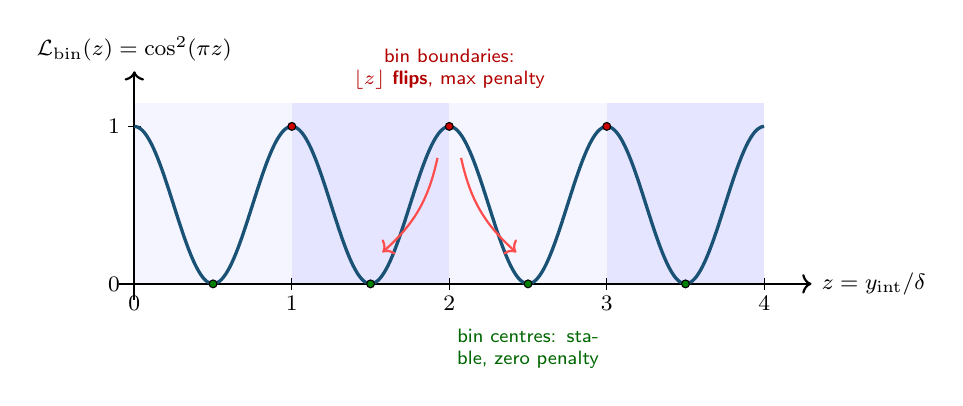
\begin{tikzpicture}[scale=1.0,
        every node/.style={font=\footnotesize}]
      % Coordinate system: x \in [0, 8] represents z \in [0, 4]
      % (so 1 unit of z is 2cm wide). Penalty cos^2(\pi z) maps to y \in [0, 2].

      % Alternating bin shading
      \fill[blue!4] (0,0) rectangle (2, 2.3);
      \fill[blue!10] (2,0) rectangle (4, 2.3);
      \fill[blue!4] (4,0) rectangle (6, 2.3);
      \fill[blue!10] (6,0) rectangle (8, 2.3);

      % Axes
      \draw[->, thick] (-0.2, 0) -- (8.6, 0)
        node[right] {$z = y_{\mathrm{int}}/\delta$};
      \draw[->, thick] (0, -0.2) -- (0, 2.7)
        node[above] {$\mathcal{L}_{\mathrm{bin}}(z) = \cos^{2}(\pi z)$};

      % Y-axis ticks
      \draw (-0.08, 2) -- (0.08, 2) node[left=4pt] {$1$};
      \draw (-0.08, 0) -- (0.08, 0) node[left=4pt] {$0$};

      % X-axis ticks at integer z (bin boundaries)
      \foreach \k/\xpos in {0/0, 1/2, 2/4, 3/6, 4/8} {
        \draw (\xpos, -0.08) -- (\xpos, 0.08);
        \node[below=1pt] at (\xpos, 0) {$\k$};
      }
      % Half-integer ticks (bin centres) -- smaller marks
      \foreach \xpos in {1, 3, 5, 7} {
        \draw[gray!60] (\xpos, -0.04) -- (\xpos, 0.04);
      }

      % The cos^2(pi z) curve.  In TikZ degree-mode, cos((pi z) rad) = cos(90 z deg).
      \draw[mybluedark, very thick, smooth, samples=200, domain=0:8]
        plot (\x, {2 * (cos(90*\x))^2});

      % Bin-boundary annotations (peaks)
      \foreach \xb in {2, 4, 6} {
        \node[draw, circle, fill=red!80!black, inner sep=1pt] at (\xb, 2) {};
      }
      \node[align=center, anchor=south, font=\scriptsize, red!70!black,
            text width=3.0cm]
        at (4, 2.35) {bin boundaries:\\
                       \textbf{$\lfloor z\rfloor$ flips},
                       max penalty};

      % Bin-centre annotations (zeros)
      \foreach \xc in {1, 3, 5, 7} {
        \node[draw, circle, fill=green!50!black, inner sep=1pt] at (\xc, 0) {};
      }
      \node[align=center, anchor=north, font=\scriptsize, green!40!black,
            text width=3.2cm]
        at (5, -0.45) {bin centres: stable, zero penalty};

      % Show "push" arrows: values near a boundary get pulled toward
      % adjacent centres.
      \draw[->, thick, red!70] (3.85, 1.6) to[bend left=18] (3.15, 0.4);
      \draw[->, thick, red!70] (4.15, 1.6) to[bend right=18] (4.85, 0.4);

    \end{tikzpicture}
    \caption{The bin-centre auxiliary loss}
    \label{fig:bin_center_penalty}
  \end{figure}

  \begin{table}[htbp]
    \centering
    \caption{INT8 calibration study on Llama-3.2-1B (128 samples,
      $\delta \approx 2016$).}
    \label{tab:int8}
    \renewcommand{\arraystretch}{1.2}
    \begin{tabular}{@{}lrr@{}}
      \toprule
      \textbf{Configuration} & \textbf{no-ADC PPL} & \textbf{ADC PPL} \\
      \midrule
      bfloat16 baseline           & ---   & \textbf{8.68}  \\
      Baseline ($\alpha = 0$)     & 10.01 & 28.86          \\
      Bin-center ($\lambda = 0.1$) & 10.01 & 28.86         \\
      Propagated ($\alpha = 1$)    & 11.01 & \textbf{14.55} \\
      Prop $+$ bin-center          & 11.00 & \textbf{14.41} \\
      \bottomrule
    \end{tabular}
  \end{table}

  Propagation alone reduces ADC PPL by $47\%$ (28.86 to 14.55) with
  no change to dead-rate, confirming that the remaining gap is ADC
  resolution rather than the dead zone.  The bin-center loss has no
  effect on its own but gives a marginal improvement ($+0.14$ PPL)
  on top of propagation.

  \paragraph{Relation to Table~\ref{tab:main_results}.}
  Table~\ref{tab:int8} is a WikiText-only calibration-objective
  ablation at 128 samples with a single calibration stage; its purpose
  is to isolate the effect of propagation and the bin-center auxiliary
  loss.  The 14.41 reported here is therefore the best WikiText-2 PPL
  achievable for this restricted setup, not a deployable checkpoint.
  The main results in Table~\ref{tab:main_results} use a different
  protocol: 1024 calibration samples and the full Stage A
  $+$ Stage B pipeline shared across all INT8/INT4 configurations so
  that the comparison across bit-widths is on a unified recipe.  Under
  that recipe the INT8 $+$ ADC PTQ checkpoint reaches WikiText-2 PPL
  $16.85$.  The two numbers are not contradictory: the staged recipe
  trades a small amount of INT8 WikiText-2 quality for the
  cross-configuration consistency required to compare bit-widths and
  to run the lm-evaluation-harness sweep, while the
  calibration-objective conclusions of Table~\ref{tab:int8}
  (propagation matters, the bin-center loss is a marginal addition)
  carry over to the deployed pipeline.

  % \begin{figure}[htbp]
  %   \centering
  %   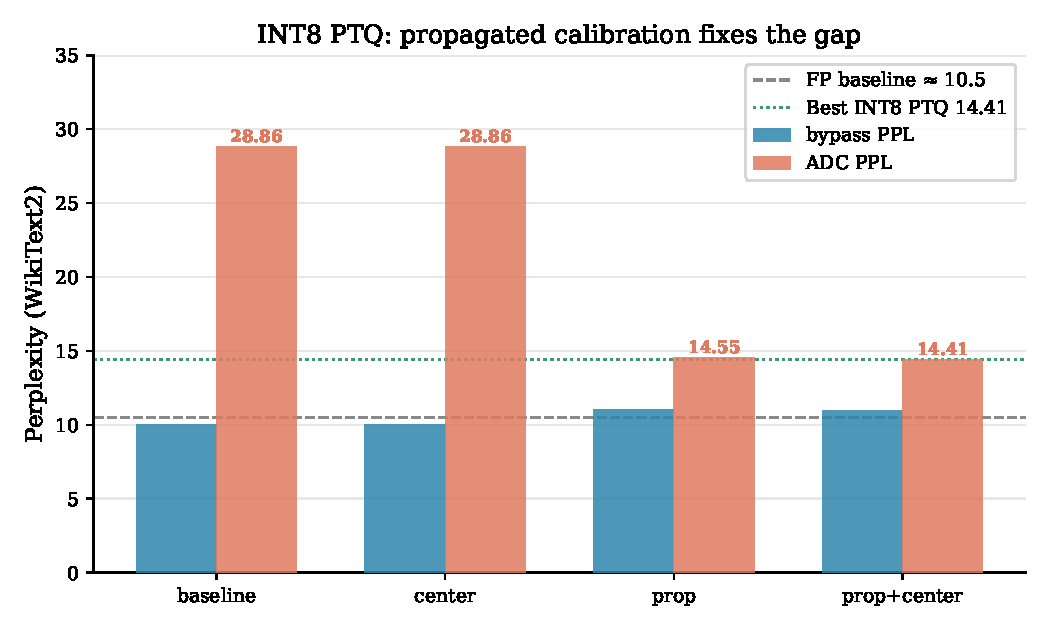
\includegraphics[width=0.7\linewidth]{plot_int8_main_results.pdf}
  %   \caption{INT8 calibration ablation. Bin-centre loss alone has no
  %     effect; propagated calibration drops ADC PPL by 47\%
  %     (28.86~$\to$~14.55) by exposing the calibration to the same
  %     ADC-distorted inputs that the model sees at inference.}
  %   \label{fig:int8_main_results}
  % \end{figure}

  \subsubsection{INT4: Sample Count and Propagation}
  \label{sec:int4_samples}

  At INT4 ($b_x = b_w = 4$) the ADC step size drops from
  $\delta \approx 2016$ at INT8 to $\delta \approx 6.12$ --- two
  orders of magnitude finer.  The no-ADC baseline reaches WikiText-2
  perplexity $15.41$, but enabling the ADC step blows it up to
  $2354.86$: a $\times 153$ gap, against $\times 2.9$ at INT8.  The
  experiments below sweep the dominant levers --- sample count,
  propagation, transform initialisation, and decoupled training ---
  on Llama-3.2-1B; Table~\ref{tab:int4v1} summarises the runs.

  Propagation was the dominant lever at INT8, so it is the natural
  first try.  At 128 samples it drops ADC perplexity to $203.89$ but
  pushes no-ADC perplexity from $15.41$ to $40.28$: the transforms
  optimise for ADC-distorted inputs at the cost of clean ones.  The
  gap narrows to $\times 5.1$ but the absolute ADC perplexity remains
  unusable, which already suggests 128 samples are too few for
  propagated INT4 calibration to generalise.

  Two orthogonal modifications reported to help in similar pipelines
  were tested next.  Replacing the random orthogonal Kronecker init
  with a Hadamard matrix~\cite{QuaRot2024}, both alone and with
  propagation, produces numbers within noise of the random-init
  counterparts at the same budget (Table~\ref{tab:int4v1}); the
  bottleneck is not where the optimiser starts.  A decoupled scheme
  --- training transforms at INT8 weights but evaluating under the
  INT4 ADC --- gives the best no-ADC perplexity of the sweep
  ($11.64$, close to INT8) but an ADC perplexity of $276.25$
  ($\times 24$ gap), because transforms tuned for the INT8 loss
  landscape do not match the much finer INT4 $\delta$.

  The dominant lever is in fact the sample count.  Raising the
  calibration set to 512 samples and rerunning propagated calibration
  yields no-ADC perplexity $34.25$ and ADC perplexity
  $\mathbf{40.63}$ ($\mathbf{\times 1.2}$ gap) --- a five-fold drop
  in ADC perplexity over the 128-sample propagated run, with the gap
  now within a few percent of the no-ADC measurement.  As a sanity
  check, the non-propagated baseline rerun at 1024 samples gives
  no-ADC $19.80$ and ADC $56.83$, a $\times 42$ ADC improvement over
  the 128-sample baseline driven purely by data.  Propagation still
  helps on top, but the experiment confirms that low-bit calibration
  is fundamentally sample-hungry: at $b_w = b_x = 4$ the calibration
  objective sees far fewer effective gradient signals per token,
  and more data is needed to span the activation distribution well
  enough for the transforms to converge.

  \begin{table}[htbp]
    \centering
    \caption{INT4 sample count and propagation sweep on Llama-3.2-1B
      ($\delta \approx 6.12$). Gap is the ratio
      ADC PPL / no-ADC PPL on WikiText-2.}
    \label{tab:int4v1}
    \renewcommand{\arraystretch}{1.15}
    \begin{tabular}{@{}lrrrl@{}}
      \toprule
      \textbf{Config} & \textbf{Samples} & \textbf{no-ADC PPL} & \textbf{ADC PPL} & \textbf{Gap} \\
      \midrule
      Baseline                       & 128  & 15.41 & 2354.86 & $\times$153 \\
      Propagated ($\alpha=1$)        & 128  & 40.28 & 203.89  & $\times$5.1 \\
      Hadamard init                  & 128  & 15.08 & 2080.51 & $\times$138 \\
      Hadamard init + prop           & 128  & 34.73 & 178.86  & $\times$5.1 \\
      Decoupled (train w8, eval w4)  & 128  & \textbf{11.64} & 276.25 & $\times$24 \\
      Propagated ($\alpha=1$)        & 512  & 34.25 & \textbf{40.63} & $\mathbf{\times 1.2}$ \\
      Baseline                       & 1024 & 19.80 & 56.83   & $\times$2.9 \\
      \bottomrule
    \end{tabular}
  \end{table}

  % \begin{figure}[htbp]
  %   \centering
  %   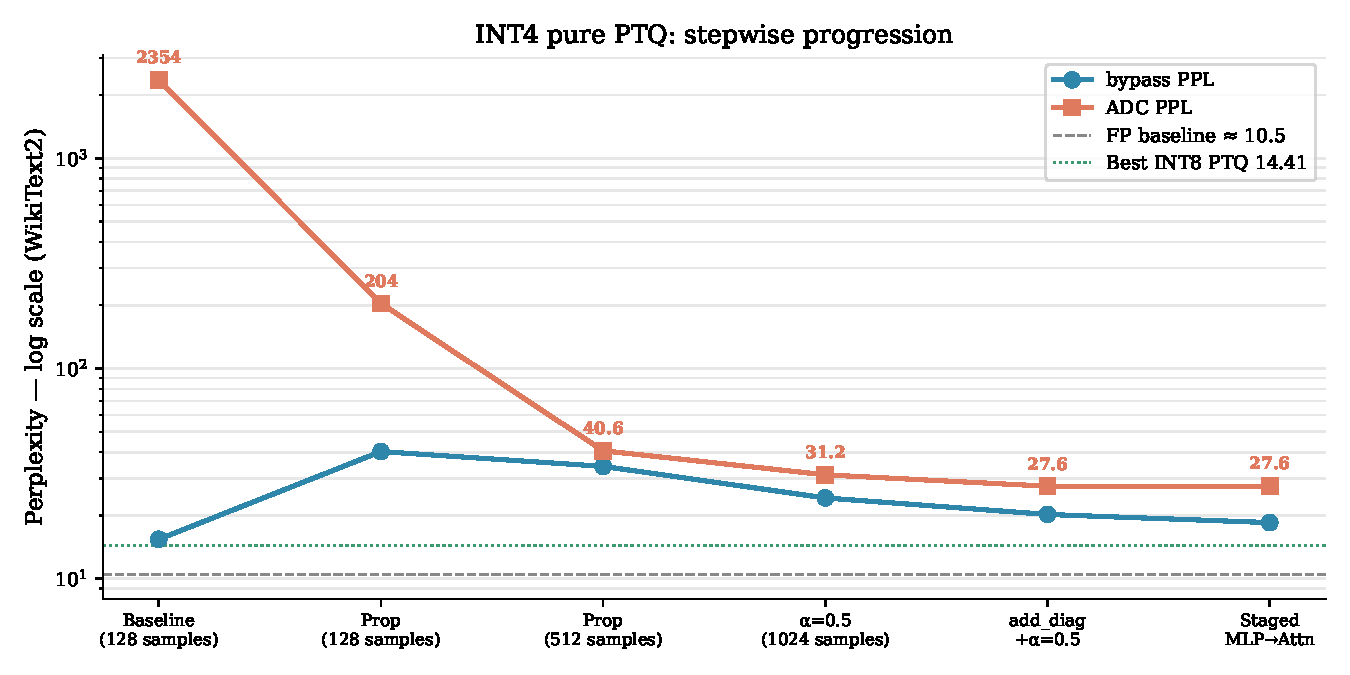
\includegraphics[width=0.75\linewidth]{plot_int4_ptq_progression.pdf}
  %   \caption{Step-by-step INT4 PTQ progression. Each step targets
  %     one failure mode: 128 samples (catastrophic, ADC PPL~2355);
  %     propagation $+$ 1024 samples (40.6); partial $\alpha=0.5$ mixing
  %     and bounded diagonals (27.56); staged training (26.66 with
  %     cleanest no-ADC~17.83). FP baseline and INT8-prop+centre
  %     reference lines are shown.}
  %   \label{fig:int4_ptq_progression}
  % \end{figure}

  \subsubsection{INT4: $\alpha$-Mixing Sweep (1024 Samples)}
  \label{sec:alpha_sweep}

  Section~\ref{sec:int4_samples} established that 1024 calibration
  samples and propagation are necessary for INT4 to generalise.  The
  natural follow-up question is what mixing weight $\alpha$ in the
  dual-forward objective
  $\mathcal{L}(\alpha) = (1{-}\alpha)\,\mathcal{L}_{\mathrm{FP}}
  + \alpha\,\mathcal{L}_{\mathrm{ADC}}$ best balances clean and
  ADC-propagated calibration.  Table~\ref{tab:int4v2} sweeps $\alpha$
  from $0$ (clean teacher only) to $1$ (fully propagated) at
  1024 samples, with three random calibration seeds per cell.

  \begin{table}[htbp]
    \centering
    \caption{INT4 $\alpha$-mixing sweep. 1024 calibration samples. Values are
             mean $\pm$ 1$\sigma$ over 3 random calibration seeds.}
    \label{tab:int4v2}
    \renewcommand{\arraystretch}{1.15}
    \begin{tabular}{@{}lrrrr@{}}
      \toprule
      \textbf{Config} & \textbf{$\alpha$} & \textbf{no-ADC PPL} & \textbf{ADC PPL} & \textbf{Gap} \\
      \midrule
      Baseline                  & 0.00 & $19.80\pm0.5$ & $56.83\pm2.5$ & $\times$2.87 \\
      Prop $\alpha=0.25$        & 0.25 & $21.65\pm0.5$ & $32.35\pm1.0$ & $\times$1.49 \\
      Prop $\alpha=0.5$         & 0.50 & $24.24\pm0.6$ & $\mathbf{31.22\pm0.9}$ & $\mathbf{\times 1.29}$ \\
      Prop $\alpha=0.75$        & 0.75 & $27.46\pm0.8$ & $35.92\pm1.2$ & $\times$1.31 \\
      Prop $\alpha=1.0$ (full)  & 1.00 & $30.32\pm1.0$ & $40.20\pm1.5$ & $\times$1.32 \\
      \bottomrule
    \end{tabular}
  \end{table}

  Figure~\ref{fig:alpha_sweep} visualises the sweep.  The minimum
  ADC perplexity is attained at $\alpha = 0.5$ (31.22, gap
  $\times 1.29$), which is also the best gap ratio in the sweep.
  Smaller values under-weight the ADC regime --- the transforms
  shape pre-ADC distributions for an objective that does not see the
  $\lfloor \cdot \rfloor$ step --- while larger values amplify
  gradient noise from the floor operator and steadily degrade no-ADC
  quality without further ADC gains.

  \begin{figure}[htbp]
    \centering
    
\includegraphics[width=0.7\linewidth]{plot_alpha_sweep.pdf}
    \caption{$\alpha$-mixing sweep at 1024 calibration samples. ADC
      PPL is minimized at $\alpha = 0.5$; smaller values
      under-weight the ADC regime, larger values amplify gradient
      noise from the floor operator and degrade no-ADC PPL.}
    \label{fig:alpha_sweep}
  \end{figure}

  % \begin{figure}[htbp]
  %   \centering
  %   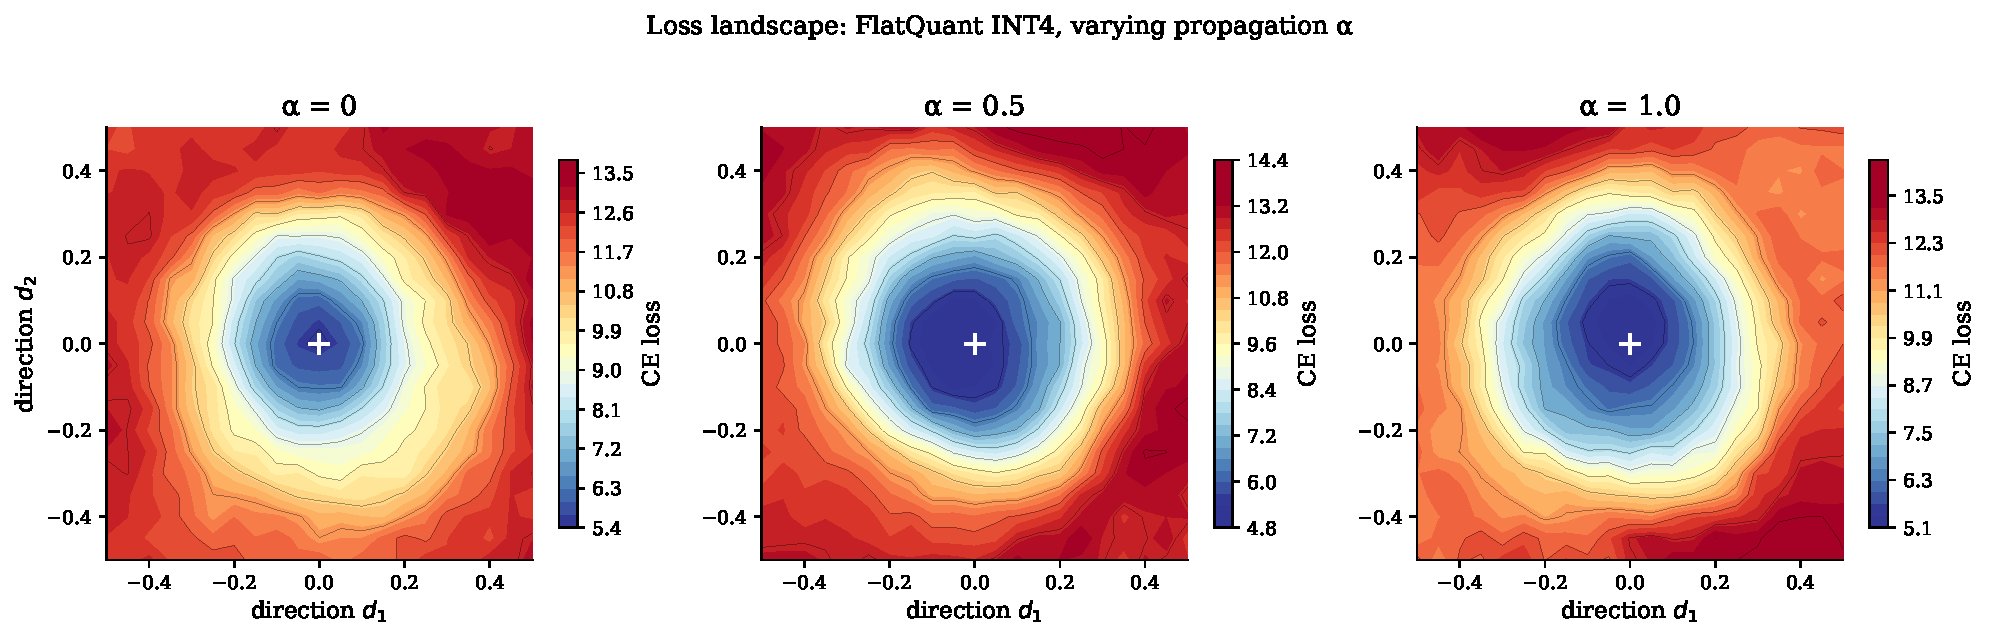
\includegraphics[width=0.85\linewidth]{plot_loss_landscape_alpha.pdf}
  %   \caption{Loss-landscape visualisation around the converged
  %     transforms for $\alpha \in \{0, 0.5, 1\}$ via filter-normalized
  %     random perturbations. The $\alpha = 0.5$ minimum is the widest
  %     and flattest, indicating that mixed FP/ADC calibration finds
  %     smoother solutions than either extreme.}
  %   \label{fig:loss_landscape}
  % \end{figure}

  \subsubsection{INT4: Diagonal Placement, MLP Decomposition, and Staged Training}
  \label{sec:int4_diagonals}

  Section~\ref{sec:int4_samples} converged to a recipe (1024 samples,
  propagation with $\alpha = 0.5$) that closes the gap to $\times 1.29$
  but is still bounded at ADC PPL $\approx 31$.  The bounded
  per-channel scaling component, inherited from FlatQuant-style
  equivalent transformations~\cite{FlatQuant2024} and used here in
  an ADC-aware setting, is the next degree of freedom on top of the
  Kronecker transforms: a per-channel scale
  $D = \mathrm{diag}(d_1, \ldots, d_c)$ with $d_i \in [10^{-4}, 10]$
  that absorbs into the surrounding weights at deployment.  The
  model has \emph{two} natural positions for such a diagonal ---
  one before the attention sub-layer (acting on $q/k/v$ inputs,
  plus a second instance before $o$) and one before the MLP
  sub-layer (acting on \texttt{gate}/\texttt{up} inputs, plus a
  second before \texttt{down}).  Table~\ref{tab:int4v3v4} ablates
  these two placements and decomposes them further.

  Reading the first block of Table~\ref{tab:int4v3v4} reveals a
  consistent pattern that is also summarised in
  Figure~\ref{fig:diag_roles}.  The MLP diagonal acts
  primarily on the transform-quality axis: enabling it alone drops
  no-ADC PPL to $19.37$ (close to its best achievable value), but
  leaves the ADC gap wide ($31.65$ ADC PPL).  
  
  The attention diagonal behaves dually: enabling it alone barely moves no-ADC
  PPL ($24.98$, worse than no diagonal) but produces a comparatively
  small ADC gap ($29.41$).  Intuitively, the MLP diagonal reshapes
  the per-channel variance of the activations that feed the
  feed-forward weight matrices --- this is where INT4 rounding
  errors are largest, so any reduction directly improves digital
  inference quality.  The attention diagonal, by contrast, mostly
  affects the magnitude of pre-ADC accumulators inside the GQA
  block, which controls how often a tile's $y_{\mathrm{int}}/\delta$
  falls into the dead-zone or saturates --- it has little leverage
  on digital quality but is essential for ADC robustness.
  Configurations that activate only one of the two leave significant
  perplexity on the table; the two diagonals are complementary, not
  redundant.

  \begin{figure}[htbp]
    \centering
    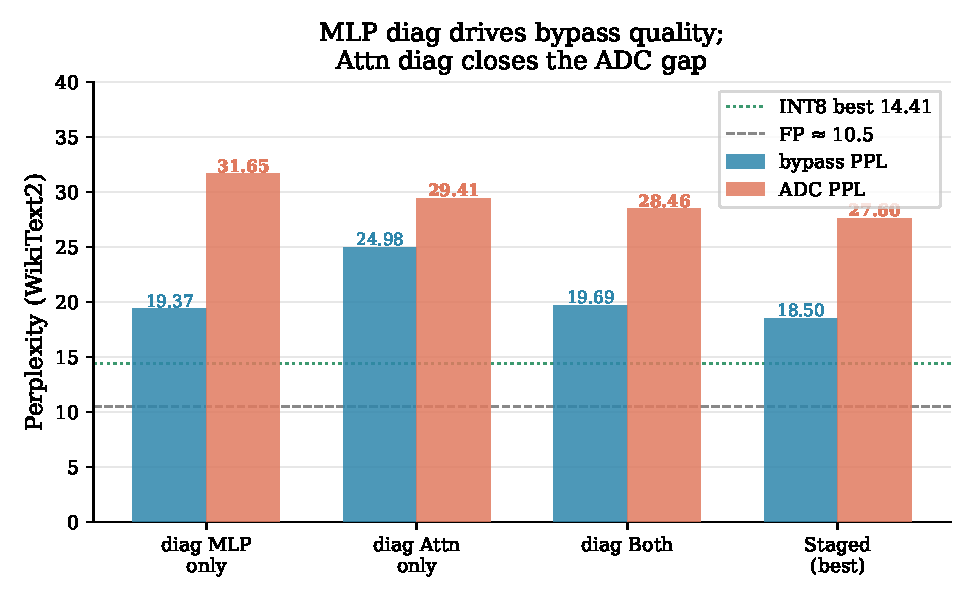
\includegraphics[width=0.62\linewidth]{plot_diag_roles.pdf}
    \caption{Roles of the MLP and attention diagonals. The MLP
      diagonal drives no-ADC PPL improvements (transform quality);
      the attention diagonal closes the no-ADC-to-ADC gap (robustness
      to ADC noise). Either alone leaves significant perplexity on
      the table; staged training combines both.}
    \label{fig:diag_roles}
  \end{figure}

  \begin{table}[htbp]
    \centering
    \caption{INT4 diagonal placement and staged training. 1024 samples,
             $\alpha=0.5$. Values are mean $\pm$ 1$\sigma$ over 3 random
             calibration seeds, except the final staged row, which
             reports the selected checkpoint used in
             Table~\ref{tab:main_results}.}
    \label{tab:int4v3v4}
    \renewcommand{\arraystretch}{1.15}
    \resizebox{\textwidth}{!}{%
    \begin{tabular}{@{}lrrl@{}}
      \toprule
      \textbf{Config} & \textbf{no-ADC PPL} & \textbf{ADC PPL} & \textbf{Note} \\
      \midrule
      Both diag (control)        & $19.69\pm0.5$ & $28.46\pm0.8$ & joint diag baseline \\
      Attn diag only             & $24.98\pm0.6$ & $29.41\pm0.8$ & worse no-ADC PPL \\
      MLP diag only              & $19.37\pm0.4$ & $31.65\pm1.0$ & best no-ADC PPL, wide gap \\
      MLP diag + layer-wise $\alpha$ & $\mathbf{19.00\pm0.4}$ & $28.66\pm0.7$ & best no-ADC PPL overall \\
      Both diag + layer-wise $\alpha$ & $19.39\pm0.4$ & $28.55\pm0.7$ & no gain over flat $\alpha$ \\
      \midrule
      \texttt{up\_gate} diag only & $23.22\pm0.7$ & $39.59\pm1.4$ & weak \\
      \texttt{down} diag only     & $20.42\pm0.5$ & $31.26\pm0.9$ & main contributor \\
      Staged: MLP diag $\to$ attn diag & \textbf{17.83} & \textbf{26.66} & \textbf{best PTQ (Table~\ref{tab:main_results})} \\
      \bottomrule
    \end{tabular}}
  \end{table}

  Inside the MLP diagonal: \texttt{down\_proj} dominates.
  The MLP diagonal can be further decomposed into the diagonal that
  precedes the \texttt{gate}/\texttt{up} projections and the one
  that precedes \texttt{down}.  The second block of
  Table~\ref{tab:int4v3v4}, visualised in
  Figure~\ref{fig:mlp_split}, shows that the two are far from equal:
  the \texttt{up\_gate} diagonal alone yields no-ADC PPL $23.22$
  with a wide gap ($39.59$ ADC), while the \texttt{down} diagonal
  alone is already close to the full-MLP setting ($20.42 / 31.26$).
  Mechanistically this is exactly what one expects: \texttt{down\_proj}
  is the last linear layer before the residual addition in each
  block, and its output is what the next block's tiles will read
  through the ADC, so a per-channel scaling here directly controls
  the conditioning of the most consequential pre-ADC signal in the
  network.  The \texttt{up}/\texttt{gate} diagonal acts on
  activations that have already passed through the FlatQuant
  rotations and the SwiGLU non-linearity, where the rotation has
  already absorbed most of the per-channel variance --- adding
  another diagonal here is largely redundant.

  Because the MLP and attention diagonals optimise different things,
  training them jointly with a single $\alpha$ creates gradient
  interference: gradients that would push the MLP diagonal toward
  a clean-input optimum compete with gradients pushing the attention
  diagonal toward ADC-robust scales.  The control row in
  Table~\ref{tab:int4v3v4} (\emph{Both diag}, ADC $28.46$) sits
  between the two single-diagonal extremes, confirming that the
  joint optimum is a compromise rather than a synthesis.

  Staged training resolves this conflict by fitting the two
  diagonals in separate phases, while keeping the Kronecker basis
  trainable throughout (Listing~\ref{lst:staged}).

  Stage~A (30 epochs at the base learning rate $\eta$) enables the
  MLP diagonal $D^{(\mathrm{m})}$ and freezes the attention
  diagonal $D^{(\mathrm{a})}$.  The Kronecker factors of all seven
  projections are optimised under the pure FP reconstruction loss
  ($\alpha = 0$), so the MLP scaling and the underlying rotations
  converge on a clean, low-variance objective without seeing any
  ADC noise; this drives the no-ADC PPL down to its best achievable
  value.

  Stage~B (10 epochs at $0.1\eta$) freezes $D^{(\mathrm{m})}$ at
  its Stage-A value and enables $D^{(\mathrm{a})}$, switching to
  the mixed objective with $\alpha = 0.5$ so that gradients flow
  through the floor operator.  The Kronecker factors remain
  trainable, but the $10\times$ smaller learning rate means the
  MLP basis is only fine-tuned around its Stage-A optimum.
  Effectively the MLP basis is held in place while the attention
  diagonal is fitted under ADC-propagated inputs --- a small,
  well-conditioned fine-tune of
  the attention block under propagated inputs --- the very signal
  the attention diagonal is supposed to reshape.

  This schedule achieves the best pure-PTQ result in our sweep:
  no-ADC PPL $17.83$ and ADC PPL $26.66$, lower than the
  single-stage joint baseline on both axes and with a tighter
  spread across calibration seeds.  The improvement is not an
  additional capacity gain over single-stage training --- the
  parameter set is identical --- but rather a direct consequence of
  separating the two sub-systems' optimisation trajectories so that
  neither pulls the other away from its natural optimum.

  \begin{figure}[htbp]
    \centering
    
\includegraphics[width=0.62\linewidth]{plot_mlp_split_up_down.pdf}
    \caption{MLP-diagonal decomposition. \texttt{down\_proj}
      contributes nearly all of the no-ADC PPL improvement; the
      \texttt{up}/\texttt{gate} diagonal contributes little, since
      \texttt{down\_proj} sits immediately before the next ADC
      accumulation and shapes the signal that is read.}
    \label{fig:mlp_split}
  \end{figure}

  \subsubsection{INT4: Stochastic Propagation}
  \label{sec:int4_stochastic}

  The deterministic $\alpha = 0.5$ objective optimises an expectation
  over a fixed, equal mixture of clean and ADC-propagated forwards.
  Section~\ref{sec:int4_diagonals} showed that this point is the best
  gap-ratio operating point of the deterministic family; the natural
  follow-up is whether replacing the constant $\alpha$ by a random
  variable $\alpha_t$ sampled per batch can improve any of the three
  measurements: no-ADC PPL, ADC PPL, or the gap.  Two stochastic
  schedules were compared with the deterministic baseline.

  The first is a deterministic mixture at $\alpha = 0.5$:
  a single dual-forward objective at fixed weight, evaluated every
  batch,
  \begin{equation}
      \mathcal{L}_{\mathrm{det}}
      \;=\;
      \tfrac{1}{2}\,\mathcal{L}_{\mathrm{FP}}(B)
      \;+\;
      \tfrac{1}{2}\,\mathcal{L}_{\mathrm{ADC}}(B).
  \end{equation}
  Every gradient step sees both losses simultaneously.  This is the
  reference configuration from Section~\ref{sec:alpha_sweep}.

  The second replaces this constant weight with Bernoulli switching
  at $p = 0.5$: at each batch $t$, a single Bernoulli draw selects
  which forward pass is executed,
  \begin{equation}
      \alpha_t \sim \mathrm{Bernoulli}(0.5),
      \qquad
      \mathcal{L}_{\mathrm{Bern}}(t)
      \;=\;
      \begin{cases}
        \mathcal{L}_{\mathrm{FP}}(B),  & \alpha_t = 0, \\
        \mathcal{L}_{\mathrm{ADC}}(B), & \alpha_t = 1.
      \end{cases}
  \end{equation}
  Only one forward through the block is performed per batch (half
  the compute of the deterministic variant), and in expectation
  $\mathbb{E}_t[\mathcal{L}_{\mathrm{Bern}}] = \mathcal{L}_{\mathrm{det}}$.
  This is the QDrop-style schedule~\cite{QDrop2022}: clean and
  ADC-propagated losses appear in alternation rather than averaged
  per batch.

  The third uses continuous $\mathrm{Beta}(2,2)$ sampling: at each
  batch a mixing weight is drawn from a symmetric Beta distribution
  concentrated around $0.5$, and the dual-forward objective is
  evaluated at that weight,
  \begin{equation}
      \alpha_t \sim \mathrm{Beta}(\beta, \beta) \;\; (\beta = 2),
      \qquad
      \mathcal{L}_{\mathrm{Beta}}(t)
      \;=\;
      (1 - \alpha_t)\,\mathcal{L}_{\mathrm{FP}}(B)
      \;+\;
      \alpha_t\,\mathcal{L}_{\mathrm{ADC}}(B).
  \end{equation}
  With $\beta = 2$ the density is peaked at $0.5$ with variance
  $1/20$, so most batches see a near-equal mixture and occasional
  batches lean slightly toward one extreme.  This is a smoother
  stochastic variant of the deterministic schedule: it preserves
  the dual-forward structure but adds light noise to the mixing
  weight.

  Each schedule was evaluated in both the flat setting
  (single-stage training, both diagonals jointly) and the
  staged setting from Section~\ref{sec:int4_diagonals}
  (Stage~A: MLP only, $\alpha = 0$; Stage~B: attention added, with
  the stochastic objective applied in Stage~B).
  Table~\ref{tab:int4v5} reports both configurations.

  \begin{table}[htbp]
    \centering
    \caption{INT4 stochastic propagation. 1024 samples. ``Mode''
      flat = single-stage joint training; staged = Stage~A/B
      schedule from Table~\ref{tab:int4v3v4} with the stochastic
      objective used in Stage~B.}
    \label{tab:int4v5}
    \renewcommand{\arraystretch}{1.15}
    \begin{tabular}{@{}llrrl@{}}
      \toprule
      \textbf{Schedule} & \textbf{Mode} & \textbf{no-ADC PPL} & \textbf{ADC PPL} & \textbf{Gap} \\
      \midrule
      Deterministic $\alpha=0.5$ & flat   & 24.24 & 31.22 & $\times$1.29 \\
      Bernoulli ($p=0.5$)        & flat   & 19.25 & 35.38 & $\times$1.84 \\
      $\mathrm{Beta}(2,2)$       & flat   & 22.90 & 31.40 & $\times$1.37 \\
      Deterministic $\alpha=0.5$ & staged & 17.83 & 26.66 & $\times$1.50 \\
      Bernoulli ($p=0.5$)        & staged & \textbf{16.94} & 32.44 & $\times$1.92 \\
      $\mathrm{Beta}(2,2)$       & staged & 17.16 & \textbf{27.82} & $\times$1.62 \\
      \bottomrule
    \end{tabular}
  \end{table}

  Two patterns emerge consistently across both modes.  First,
  Bernoulli switching gives the best \emph{no-ADC} perplexity in
  each mode ($19.25$ flat, $\mathbf{16.94}$ staged) but the worst
  ADC gap ($\times 1.84$ and $\times 1.92$).  This follows directly
  from the schedule's structure: in batches with $\alpha_t = 0$ the
  attention transforms see no ADC signal and drift toward
  configurations that minimise the clean loss without any pressure
  to be ADC-robust, while in batches with $\alpha_t = 1$ the
  optimiser has to compensate for that drift.  The two regimes
  partially cancel, but the residual drift toward clean-loss optima
  improves no-ADC quality at the cost of ADC robustness.

  Second, $\mathrm{Beta}(2,2)$ behaves almost identically to the
  deterministic schedule.  Because the Beta(2,2) density is peaked
  near $0.5$ with low variance, the per-batch mixing weights cluster
  tightly around the deterministic value, and the resulting trained
  transforms differ from the deterministic baseline only by an
  amount commensurate with run-to-run noise.  The marginal ADC
  difference in the staged setting ($27.82$ vs $26.66$) is within
  one standard deviation across calibration seeds and does not
  justify the additional per-batch sampling.

  Taken together, the stochastic schedules do not displace the
  deterministic $\alpha = 0.5$ recipe.  The deterministic staged
  configuration remains the best PTQ result on the
  no-ADC--vs--ADC Pareto front: it matches the staged-Beta ADC PPL
  without the noisier gradients, and it dominates the staged-Bernoulli
  configuration on the ADC axis even though Bernoulli is better on
  no-ADC.  We therefore retain deterministic $\alpha = 0.5$ as the
  default mixing schedule for all downstream experiments.

  \subsubsection{Post-ADC Residual LoRA: Initial Sweep}
  \label{sec:lora_initial}

  Table~\ref{tab:lorav6} evaluates LoRA adapters on top of the best
  PTQ checkpoint (the staged configuration, ADC PPL $26.66$),
  varying rank and target projection sets. The corresponding parameter overhead for each
  configuration is reported in Table~\ref{tab:lora_overhead}: rank-$4$
  adapters on all seven projections add $2.82$M parameters
  ($0.228\%$ of the base model), doubling the rank doubles this
  count, and restricting the targets to \texttt{down} and
  \texttt{o\_proj} reduces the overhead to $0.92$M parameters
  ($0.074\%$).

  \begin{table}[htbp]
    \centering
    \caption{Post-ADC LoRA overhead for Llama-3.2-1B
             ($d_{\mathrm{model}}=2048$, $d_{\mathrm{ffn}}=8192$,
             $d_{\mathrm{kv}}=512$, 16 layers).}
    \label{tab:lora_overhead}
    \renewcommand{\arraystretch}{1.15}
    \begin{tabular}{@{}lrrrr@{}}
      \toprule
      \textbf{Target} & \textbf{rank} & \textbf{added params} & \textbf{\% of model} & \textbf{extra MACs/token} \\
      \midrule
      all 7 projections                & 4 & $2.82$M & $0.228\%$ & $2.82$M \\
      all 7 projections                & 8 & $5.64$M & $0.456\%$ & $5.64$M \\
      \texttt{down} + \texttt{o\_proj} & 4 & $0.92$M & $0.074\%$ & $0.92$M \\
      \bottomrule
    \end{tabular}
  \end{table}

  \begin{table}[htbp]
    \centering
    \caption{LoRA initial sweep. Base PTQ: no-ADC $17.83$, ADC $26.66$.}
    \label{tab:lorav6}
    \renewcommand{\arraystretch}{1.15}
    \begin{tabular}{@{}llrrl@{}}
      \toprule
      \textbf{Config} & \textbf{Targets} & \textbf{no-ADC PPL} & \textbf{ADC PPL} & \textbf{Gap} \\
      \midrule
      No LoRA (base PTQ) & — & 17.83 & 26.66 & $\times$1.50 \\
      LoRA $r=4$, \texttt{down}     & 1 proj & 19.33 & 16.32 & $\times$0.84 \\
      LoRA $r=8$, \texttt{down}     & 1 proj & 19.17 & 15.79 & $\times$0.82 \\
      LoRA $r=4$, \texttt{down+o}   & 2 proj & 18.68 & \textbf{15.63} & $\times$0.84 \\
      LoRA $r=4$, all 7 proj        & 7 proj & \textbf{17.73} & 16.53 & $\times$0.93 \\
      \bottomrule
    \end{tabular}
  \end{table}

  Across all LoRA configurations ADC PPL falls below no-ADC PPL (gap $<1$),
  confirming that the adapter learns to specifically correct ADC noise.
  Adding \texttt{o\_proj} to \texttt{down\_proj} gives the best ADC PPL
  (15.63); covering all 7 projections gives the best no-ADC PPL (17.73) at
  the cost of a slightly wider gap.

  \subsubsection{Post-ADC Residual LoRA: Ablation Study}

  Table~\ref{tab:lorav7} reports the full ablation across rank, loss,
  target projections, layer coverage, and adapter placement (all runs
  use $r=4$ unless stated; the \textbf{Targets} column makes the
  set of projections explicit for each row).

  \begin{table}[htbp]
    \centering
    \caption{LoRA ablation study. Llama-3.2-1B, INT4. Targets:
      \texttt{down+o} = down-projection of MLP plus output projection
      of attention; all 7 = all seven projections per block.}
    \label{tab:lorav7}
    \renewcommand{\arraystretch}{1.15}
    \begin{tabular}{@{}l l l r@{}}
      \toprule
      \textbf{Axis} & \textbf{Setting} & \textbf{Targets} & \textbf{ADC PPL} \\
      \midrule
      \multirow{3}{*}{Seed (CE)}
        & seed 1 & down+o & 15.79 \\
        & seed 2 & down+o & 15.88 \\
        & seed 3 & down+o & 15.93 \\
      \midrule
      \multirow{4}{*}{Rank (CE)}
        & $r=1$ & down+o & 15.90 \\
        & $r=2$ & down+o & 15.60 \\
        & $r=4$ & down+o & \textbf{15.57} \\
        & $r=8$ & down+o & 15.24 \\
      \midrule
      \multirow{4}{*}{Loss $\times$ Targets}
        & CE only        & down+o & 15.63 \\
        & CE $+$ KL      & down+o & 14.33 \\
        & CE only        & all 7  & 16.68 \\
        & CE $+$ KL      & all 7  & \textbf{14.03} \\
      \midrule
      \multirow{3}{*}{Layer coverage (CE)}
        & first 8 layers & down+o & 16.64 \\
        & all 16 layers  & down+o & \textbf{15.63} \\
        & last 8 layers  & down+o & 20.08 \\
      \midrule
      \multirow{2}{*}{Placement (CE)}
        & post-ADC (proposed) & down+o & \textbf{15.63} \\
        & pre-ADC             & down+o & 105.63 \textit{(diverged)} \\
      \bottomrule
    \end{tabular}
  \end{table}

  Rank saturates at $r=4$ (only 0.33 PPL gap to $r=8$).
  CE$+$KL outperforms CE alone by $1.30$ PPL with \texttt{down+o}
  targets ($15.63 \to 14.33$) and by $2.65$ PPL with all-7 targets
  ($16.68 \to 14.03$); the FP teacher signal is most useful when the
  adapter covers more projections.
  Earlier layers carry more accumulated ADC error: first-8 (16.64) beats
  last-8 (20.08).
  Pre-ADC placement diverges (ADC PPL~105.6) because the
  correction is itself quantized by the fixed $\delta$.
  The best single configuration is all 7 targets, CE$+$KL, $r=4$: ADC
  PPL $14.03$, beating the deployed INT8 + ADC PTQ checkpoint
  ($16.85$, Table~\ref{tab:main_results}).

  % \begin{figure}[htbp]
  %   \centering
  %   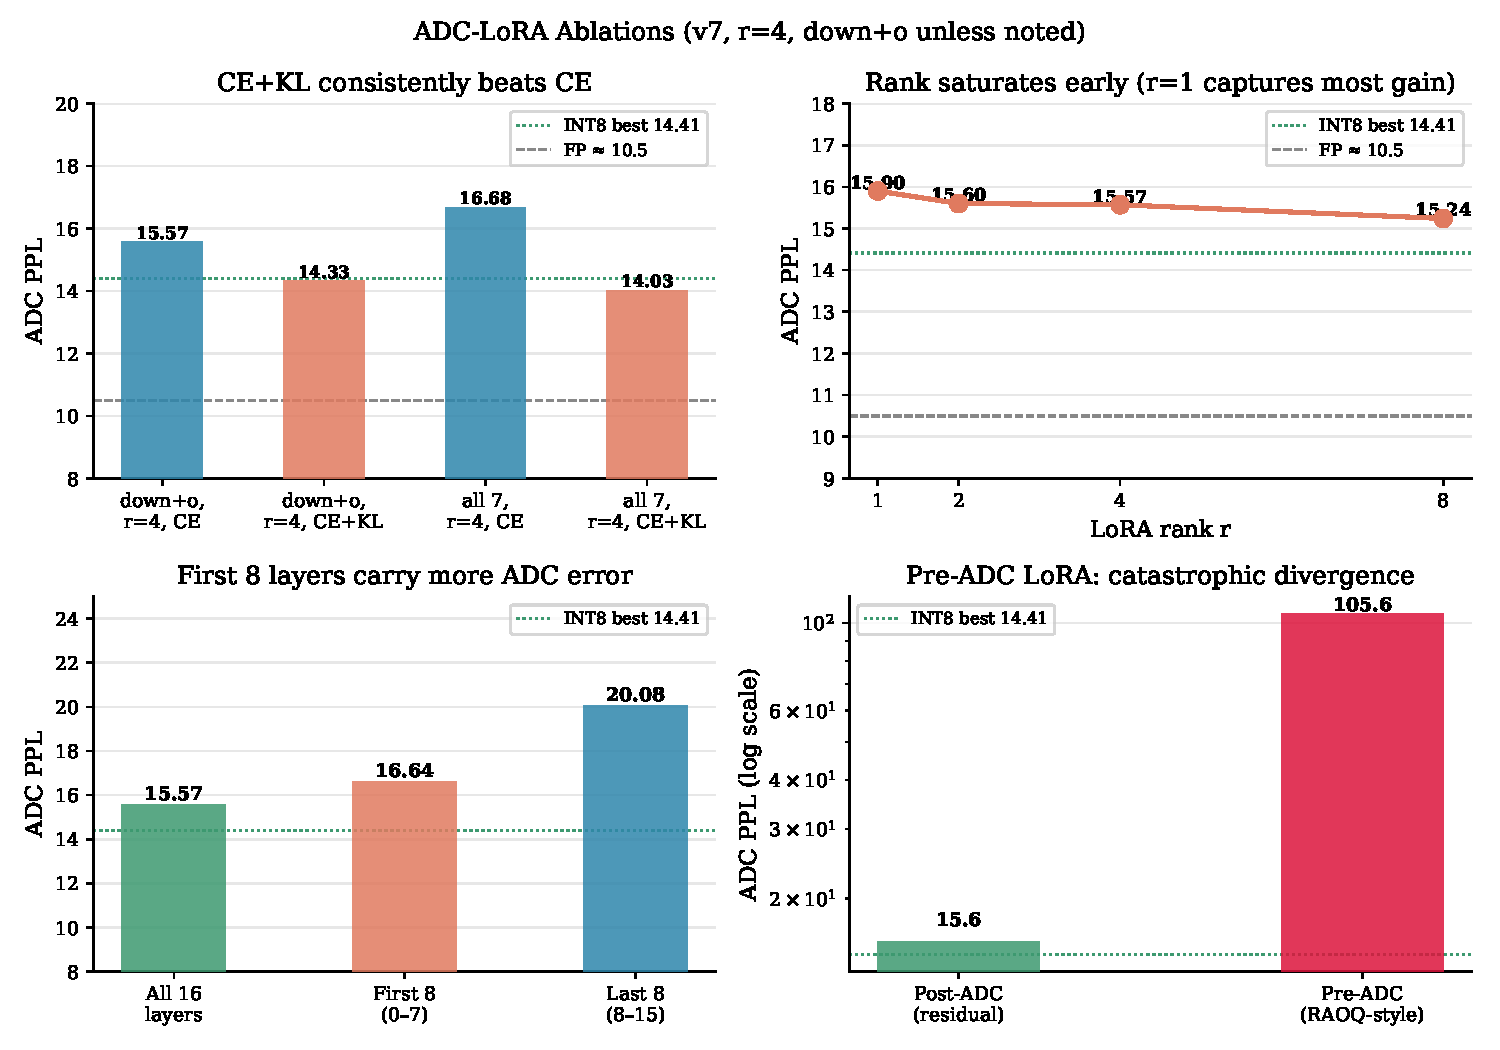
\includegraphics[width=0.85\linewidth]{plot_lora_ablations_grid.pdf}
  %   \caption{LoRA ablation grid. \emph{Top-left}: CE+KL beats CE
  %     across both target sets. \emph{Top-right}: rank saturates near
  %     $r=4$. \emph{Bottom-left}: layer coverage: first-8 beats
  %     last-8, all-16 is best, confirming that ADC error accumulates
  %     across depth. \emph{Bottom-right}: pre-ADC placement diverges,
  %     post-ADC is stable from epoch~1.}
  %   \label{fig:lora_ablations}
  % \end{figure}

  \subsubsection{Post-ADC Residual LoRA: Generalization to C4}
  \label{sec:lora_c4}

  Table~\ref{tab:lorav8} evaluates the top-3 configurations on both
  WikiText-2 and C4 to test out-of-domain transfer.

  \begin{table}[htbp]
    \centering
    \caption{LoRA generalization. WikiText-2 and C4 perplexity.}
    \label{tab:lorav8}
    \renewcommand{\arraystretch}{1.15}
    \begin{tabular}{@{}lrrrr@{}}
      \toprule
      \textbf{Config} & \textbf{Wiki no-ADC} & \textbf{Wiki ADC} & \textbf{C4 no-ADC} & \textbf{C4 ADC} \\
      \midrule
      PTQ (no LoRA)              & 17.83 & 26.66 & 28.58 & 45.62 \\
      $r=8$, \texttt{down+o}, CE & 18.51 & 15.47 & 30.48 & 29.39 \\
      $r=4$, \texttt{down+o}, CE+KL & 19.05 & 14.27 & 29.37 & 23.88 \\
      $r=4$, all 7, CE+KL        & \textbf{18.61} & \textbf{14.03} & \textbf{29.14} & \textbf{23.20} \\
      \bottomrule
    \end{tabular}
  \end{table}

  CE+KL configurations reduce C4 ADC PPL by roughly half relative to
  the PTQ baseline ($45.62 \to 23.20$) despite being calibrated solely
  on WikiText-2.  CE-only ($r=8$, \texttt{down+o}) shows much weaker
  C4 generalization ($29.39$ vs.\ $23.20$).  The KL teacher signal is
  therefore the dominant factor for cross-domain transfer.
  All-7 CE+KL is the best overall checkpoint on both datasets.

  % \begin{figure}[htbp]
  %   \centering
  %   
\includegraphics[width=0.7\linewidth]{plot_final_results_wiki_c4.pdf}
  %   \caption{Final results across configurations on WikiText-2 and
  %     C4. INT4~$+$~LoRA (all-7, CE$+$KL, $r=4$) surpasses the
  %     deployed INT8 + ADC PTQ checkpoint on WikiText-2
  %     (14.03 vs.\ 16.85) and halves the C4
  %     ADC PPL relative to the INT4 PTQ baseline (45.62~$\to$~23.20).
  %     INT8 C4 is not reported in this configuration; the C4
  %     comparison is against the INT4 PTQ baseline.}
  %   \label{fig:final_results}
  % \end{figure}

  \subsection{Unsigned Shift-Subtract Readout: A Second Hardware Setting}
  \label{sec:unipolar}

  All experiments described so far use the Signed readout: the
  analog crossbar accumulates a signed integer dot product
  $y_{\mathrm{int}} \in [-M q_x q_w,\, +M q_x q_w]$ and the ADC reads
  both positive and negative values.  A physically important alternative is an
  \emph{unsigned shift-subtract readout}.  Here the signed INT4
  activation and weight codes are first shifted to unsigned codes
  in $[0, 15]$, the array performs a single non-negative MVM, the
  ADC quantises the unsigned accumulated value, and the
  deterministic zero-point terms are subtracted digitally after
  readout.  We refer to this setting as \textbf{Unsigned}.  Real
  crossbar hardware is often constrained to non-negative currents,
  making the Unsigned setting the more realistic operating regime.
  The two readouts share the same bit-width $b_a = 8$ and tile
  size $M = 256$, but they differ in the ADC input range and in
  how the signed dot product is recovered, which changes $\delta$
  by more than a factor of two and requires a different calibration
  objective.  The Unsigned setting is therefore treated as a
  self-contained experiment series with its own baselines,
  calibration, and ablation structure.

  \subsubsection{Unsigned Shift-Subtract ADC Algorithm}
  \label{sec:unipolar_algo}

  Because the crossbar accepts only $[0, 2^b-1]$ codes, the Unsigned
  readout uses an offset-binary 4-bit codebook
  $\hat{x}^u, \hat{w}^u \in [0, 15]$ with zero point
  $z = 2^{b_x - 1} = 8$.  The corresponding centered integer codes
  $\hat{x} = \hat{x}^u - z$ and $\hat{w} = \hat{w}^u - z$ therefore
  lie in $[-8, 7]$ --- a 16-level range used only for the Unsigned
  hardware path, in place of the symmetric $q_{\mathrm{max}} = 7$
  convention of Table~\ref{tab:hardware} used by the Signed
  reference.  The deterministic zero-point terms are subtracted
  digitally after the ADC; as Step 4 shows, this correction is
  algebraically exact for the shift terms, while ADC rounding and
  clipping error remains.
  The algorithm proceeds in five steps.

  Step 1 — Shift to unsigned.
  Each signed code is offset by the zero-point $z = 2^{b_x - 1} = 8$:
  \[
    \hat{x}^u = \hat{x} + 8 \;\in [0, 15], \qquad
    \hat{w}^u = \hat{w} + 8 \;\in [0, 15].
  \]

  Step 2 — Hardware MVM.
  The crossbar computes the non-negative dot product over one tile of
  width $M = 256$:
  \[
    y^u = \langle \hat{x}^u,\, \hat{w}^u \rangle \;\in\; [0,\; M(2^{b_x}-1)(2^{b_w}-1)]
        = [0,\; 57600].
  \]
  Because $y^u \ge 0$ always, a single unsigned MVM suffices with no
  four-quadrant splitting.

  Step 3 — ADC floor.
  Because the unsigned codes span the range $[0, 2^{b_a}-1]$ rather
  than the symmetric $[-2^{b_a-1}, 2^{b_a-1}-1]$ of the Signed
  readout, the unsigned step size is:
  \[
    \delta_u = \frac{M\,(2^{b_x}-1)\,(2^{b_w}-1)}{(2^{b_a}-1)\,k}
             = \frac{256 \cdot 15 \cdot 15}{255 \cdot 16} \approx 14.1
    \quad (k = 16),
  \]
  and the quantized output is
  $\hat{y}^u = \delta_u \cdot \mathrm{clip}\!\left(\lfloor y^u / \delta_u \rfloor,\,0,\,2^{b_a}-1\right)$.
  Note that $\delta_u \approx 14.1$ is more than twice the Signed
  $\delta \approx 6.12$ at the same $k$, reflecting the fact that the
  same number of ADC bins now covers a range roughly $2\times$ wider
  in absolute terms.

  Step 4 — Digital zero-point correction.
  Expanding the unsigned product gives
  $\hat{x}^u \hat{w}^u
   = \hat{x}\hat{w} + 8\hat{w} + 8\hat{x} + 64$,
  so in the absence of any ADC quantisation the unsigned shift can be
  undone algebraically:
  \[
    y_{\mathrm{int}} \;=\; y^u
      \;-\; 8\!\sum_j \hat{w}^u_j
      \;-\; 8\!\sum_i \hat{x}^u_i
      \;+\; M \cdot 64.
  \]
  In the actual pipeline, however, the correction is applied to the
  ADC-quantised readout $\hat{y}^u$ rather than to $y^u$ itself.
  Substituting $\hat{y}^u$ into the same expression yields
  \[
    \tilde{y}_{\mathrm{int}}
      \;=\; \hat{y}^u
        - 8\!\sum_j \hat{w}^u_j
        - 8\!\sum_i \hat{x}^u_i
        + M \cdot 64
      \;=\; y_{\mathrm{int}}
            \;+\; \bigl(\hat{y}^u - y^u\bigr),
  \]
  where the residual $(\hat{y}^u - y^u)$ is the ADC rounding / clipping
  error.  The zero-point shift is therefore removed \emph{exactly}, but
  the ADC quantisation error remains uncorrected: ``exact'' here
  refers only to the algebraic shift, not to the full post-ADC
  accumulator.  This is precisely why the Unsigned setting is harder
  than the Signed one --- the coarser $\delta_u$ enlarges the residual
  $(\hat{y}^u - y^u)$, motivating the per-layer $k$ search of
  Section~\ref{sec:unipolar} and the post-ADC LoRA correction of
  Section~\ref{sec:method}.
  Both summands $\sum_j \hat{w}^u_j$ and $\sum_i \hat{x}^u_i$ are
  cheap: the weight sum is precomputed once at load time, and the
  token sum is a single reduction per token.

  Step 5 — Dequantisation.
  $y_{\mathrm{real}} = \tilde{y}_{\mathrm{int}} \cdot s_x \cdot s_w$, where
  $\tilde{y}_{\mathrm{int}}$ is the ADC-corrupted recovered accumulator
  from Step 4, $s_x$ is the per-token activation scale, and $s_w$ is
  the per-channel weight scale, exactly as in the Signed setting.

  \subsubsection{Per-Layer $k$ Search}

  Because the coarser $\delta_u$ (at global $k = 16$) imposes a
  heavier resolution penalty than the Signed setting, a per-layer
  $k$ search is introduced that selects the ADC scaling factor
  independently for each projection layer.

  Per-layer reconfiguration of the analog read-out is not assumed
  to be a universal hardware property, but such configurable setups
  do exist --- hybrid optical-electronic architectures, for
  instance, let the digital controller program per-layer parameters
  before each layer is launched~\cite{Spall2022HybridOptical}.
  Treating $k$ as a per-projection knob is consistent with the
  design space exposed by such setups; no specific accelerator is
  claimed to implement a per-layer $k$ in exactly the form used
  here, and the parameter is treated only as a deployment-time
  configuration vector.

  Operationally, our per-layer $k$ search is therefore a
  calibration-time procedure: weights and FlatQuant transforms are
  kept frozen, and only the per-projection $k$ is chosen from a
  fixed candidate set by minimising ADC reconstruction error
  against the FP teacher.  The selected $k$ values become a
  deployment-time configuration vector that costs nothing at
  inference --- $k$ is a register, not a trained parameter --- but
  recovers a meaningful fraction of the perplexity that a single
  global $k$ leaves on the table for Unsigned deployment.

  After FlatQuant calibration with a global $k$, the pre-ADC
  activations $y^u_\ell$ are captured on the calibration set for each
  projection layer $\ell$. For each candidate $k \in \mathcal{K} = \{4,
  8, 16, 32, 64\}$ the ADC reconstruction MSE is evaluated
  \[
    \mathrm{MSE}_\ell(k) \;=\; \mathbb{E}\!\left[
      \bigl( Q^{(k)}_{\mathrm{ADC}}(y^u_\ell) - y^u_\ell \bigr)^2
    \right],
  \]
  where $Q^{(k)}_{\mathrm{ADC}}$ uses $\delta_u(k)$ from
  Sec.~\ref{sec:unipolar}, and select
  \[
    k^*_\ell \;=\; \arg\min_{k \in \mathcal{K}} \mathrm{MSE}_\ell(k).
  \]
  Because $\delta_u$ is inversely proportional to $k$, this procedure
  selects the largest $k$ whose representable range still covers the
  typical magnitude of $y^u_\ell$ without saturating. Layers with
  narrow output distributions therefore receive a large
  $k$ (finer $\delta_u$, range is not needed); layers with wide
  distributions receive a small $k$ (coarser $\delta_u$ but
  wider range, avoiding saturation). The search is run in place on
  the fixed PTQ checkpoint without retraining FlatQuant transforms.

  \subsubsection{Calibration Objective for the Unsigned Readout}

  FlatQuant transforms calibrated for the Signed
  $\delta \approx 6.12$ are mismatched to the Unsigned
  $\delta_u \approx 14.1$: the transforms shape the pre-ADC signal
  for a finer resolution that the hardware does not provide.  In
  the Unsigned series, FlatQuant is therefore retrained with the
  unsigned $\delta_u$ formula as the active ADC step during
  calibration.  All other settings (staged training,
  $\alpha = 0.5$, diagonal scaling) are carried over from the best
  Signed configuration.

  \subsubsection{Experiment Configurations}

  The following seven configurations are evaluated for
  Llama-3.2-1B on WikiText-2 and C4.  We give each a
  human-readable name used in the main text and keep the original
  short identifier (in \texttt{typewriter}) in parentheses, since
  it also labels the corresponding row in Table~\ref{tab:unipolar}.
  \begin{itemize}
    \item \textbf{bfloat16 baseline} (\texttt{fp}) --- full-precision
      reference, no quantisation.
    \item \textbf{INT4 FlatQuant, ADC disabled} (\texttt{int4\_no\_adc})
      --- INT4 FlatQuant with the ADC floor turned off.  Measures the
      FlatQuant transform quality alone; trained with the Signed
      formula so the calibration does not see ADC noise, giving
      WikiText-2 PPL $12.56$.
    \item \textbf{Unsigned PTQ} (\texttt{best\_ptq}) --- INT4
      FlatQuant retrained from scratch with the unsigned $\delta_u$
      formula at global $k = 16$.
    \item \textbf{Unsigned PTQ + per-layer $k$ search}
      (\texttt{best\_ptq\_k}) --- the Unsigned PTQ checkpoint above
      with per-layer $k$ chosen in-place from the calibration
      statistics, without retraining FlatQuant.
    \item \textbf{Unsigned PTQ + per-layer $k$ + FlatQuant retraining}
      (\texttt{best\_ptq\_k\_recal}) --- the same per-layer $k$
      vector as the previous row, followed by retraining FlatQuant
      with those $k$ values baked in; tests whether retrained
      transforms improve over the in-place search.
    \item \textbf{Unsigned PTQ + post-ADC LoRA} (\texttt{best\_lora})
      --- the Unsigned PTQ checkpoint plus a post-ADC residual LoRA
      branch ($r = 4$, all seven projections, CE$+$KL loss,
      $\lambda = 0.5$, temperature $2.0$, $5$ epochs at $10^{-4}$).
    \item \textbf{Unsigned PTQ + per-layer $k$ + post-ADC LoRA}
      (\texttt{best\_lora\_k}) --- the same LoRA branch trained on
      top of the per-layer $k$ checkpoint.  This is the final
      configuration of the Unsigned series.
  \end{itemize}

  \subsubsection{Experiment History and Hardware Setting Evolution}

  The Unsigned configuration adopted above is the endpoint of two
  earlier hardware-setting iterations.  They are documented here
  so that the choice of the final configuration is not arbitrary;
  Table~\ref{tab:hardware_evolution} summarises the comparison
  before the per-layer $k$ search and LoRA correction are
  applied.

  \begin{table}[htbp]
    \centering
    \caption{Hardware-setting evolution on Llama-3.2-1B, staged
      PTQ baseline only (no per-layer $k$ search, no LoRA; the
      corresponding row in Table~\ref{tab:unipolar} is
      \texttt{best\_ptq}).  ``Cost'' is the number of ADC reads per
      tile relative to the Signed reference.}
    \label{tab:hardware_evolution}
    \renewcommand{\arraystretch}{1.2}
    \begin{tabular}{@{}lrrrc@{}}
      \toprule
      \textbf{Hardware setup} & $\boldsymbol{\delta}$ &
        \textbf{Wiki PPL} & \textbf{C4 PPL} &
        \textbf{Cost} \\
      \midrule
      Signed readout                       & $\approx 6.12$         & 26.66 & 45.62 & $1\times$ \\
      Four-read unsigned decomposition     & $\approx 3.06$/branch  & \textbf{18.08} & \textbf{28.41} & $\mathbf{4\times}$ \\
      Single-read unsigned shift-subtract  & $\approx 14.06$        & 39.00 & 67.78 & $1\times$ \\
      \bottomrule
    \end{tabular}
  \end{table}

  The starting point is the Signed readout studied in the previous
  subsections, which reads a signed accumulation
  $y_{\mathrm{int}} \in [-M q_x q_w,\, +M q_x q_w]$ directly and uses
  the step-size formula $\delta = 2 M q_x q_w / (2^{b_a} k) \approx 6.12$
  at $k = 16$.
  Under this setting the staged PTQ baseline reaches WikiText-2
  perplexity $26.66$ and post-ADC LoRA reaches $14.03$ --- the
  reference numbers for any hardware that can perform a signed
  analog accumulation directly.  In practice, however, most
  physically realisable optical and in-memory crossbars accept only
  non-negative inputs, so the Signed readout is best read as an
  idealised reference rather than a deployable target.

  A first attempt to bridge to non-negative hardware was the
  four-read unsigned decomposition, in which the signed codes are split
  into their positive and negative parts,
  \begin{equation}
      \hat{x} = \hat{x}^{+} - \hat{x}^{-},
      \qquad
      \hat{w} = \hat{w}^{+} - \hat{w}^{-},
      \qquad
      \hat{x}^{\pm}, \hat{w}^{\pm} \geq 0,
  \end{equation}
  so that the signed inner product decomposes into four products
  of non-negative tensors,
  \begin{equation}
      \langle \hat{x}, \hat{w} \rangle
      \;=\;
      \langle \hat{x}^{+}, \hat{w}^{+} \rangle
      \;+\; \langle \hat{x}^{-}, \hat{w}^{-} \rangle
      \;-\; \langle \hat{x}^{+}, \hat{w}^{-} \rangle
      \;-\; \langle \hat{x}^{-}, \hat{w}^{+} \rangle.
      \label{eq:four_quadrant}
  \end{equation}
  Each of the four terms is a non-negative MVM that can be
  executed on the crossbar directly; the signed result is then
  assembled digitally.  The branchwise step size
  $\delta_{\mathrm{branch}} \approx 3.06$ is twice as fine as the
  Signed reference, and the staged PTQ accordingly improved to
  $18.08$ WikiText-2 PPL ($28.41$ on C4).  The catch is that each
  layer now requires $4\times$ as many ADC reads, which roughly
  quadruples the dominant area-and-energy cost of the analog path
  and renders this option uncompetitive even though the perplexity
  is excellent.

  The final iteration is the single-read unsigned shift-subtract
  scheme used in the rest of this section: both code tensors are
  lifted to $[0, 2^{b} - 1]$ via the zero-point shift, a single
  non-negative MVM is executed on the hardware, and the
  deterministic zero-point terms are subtracted digitally, while the
  ADC rounding and clipping error remains as described in
  Section~\ref{sec:unipolar_algo}.  The MVM cost returns to one
  ADC read per tile, and FlatQuant is retrained from scratch with
  the matching unsigned $\delta_u$ formula so that calibration and
  deployment use the same $\delta$ throughout.
  Table~\ref{tab:unipolar} summarises the results.  At global
  $k = 16$ the Unsigned PTQ baseline gives $39.00 / 67.78$ on
  Wiki / C4 --- coarser than the Signed reference, as expected from
  the factor-of-two-larger $\delta_u$ --- but the rest of the
  toolbox is then available.  Adding the per-layer $k$ search
  (Unsigned PTQ $+$ per-layer $k$) lowers this to $21.64 / 33.79$;
  the post-ADC LoRA on top of the global-$k$ checkpoint
  (Unsigned PTQ $+$ post-ADC LoRA) reaches $17.29 / 29.26$; and
  combining both (Unsigned PTQ $+$ per-layer $k$ $+$ post-ADC LoRA)
  gives the final $\mathbf{14.56} / \mathbf{23.78}$ --- within
  striking distance of the idealised Signed LoRA reference without
  increasing the number of analog MVM / ADC reads, aside from the
  small digital LoRA overhead reported in
  Table~\ref{tab:lora_overhead}.  Re-training FlatQuant on the
  per-layer $k$ values found by the search (Unsigned PTQ $+$
  per-layer $k$ $+$ FlatQuant retraining, $22.19 / 36.94$) is in
  fact slightly worse than the in-place search: fitting the
  transforms to a specific $k$ vector over-specialises them and
  hurts generalisation, so the in-place variant is preferred.

  \begin{table}[htbp]
    \centering
    \caption{Unsigned shift-subtract readout results on
             Llama-3.2-1B. $\delta_u \approx 14.1$ at global $k = 16$.}
    \label{tab:unipolar}
    \renewcommand{\arraystretch}{1.2}
    \begin{tabular}{@{}llrr@{}}
      \toprule
      \textbf{Configuration} & \textbf{Short ID} & \textbf{Wiki PPL} & \textbf{C4 PPL} \\
      \midrule
      bfloat16 baseline                           & \texttt{fp}                  & \textbf{8.68}  & \textbf{13.13} \\
      INT4 FlatQuant, ADC disabled                & \texttt{int4\_no\_adc}       & 12.56          & 20.13          \\
      Unsigned PTQ ($k = 16$)                     & \texttt{best\_ptq}           & 39.00          & 67.78          \\
      Unsigned PTQ $+$ per-layer $k$              & \texttt{best\_ptq\_k}        & 21.64          & 33.79          \\
      Unsigned PTQ $+$ per-layer $k$ $+$ FQ retrain & \texttt{best\_ptq\_k\_recal} & 22.19          & 36.94          \\
      Unsigned PTQ $+$ post-ADC LoRA              & \texttt{best\_lora}          & 17.29          & 29.26          \\
      Unsigned PTQ $+$ per-layer $k$ $+$ post-ADC LoRA & \texttt{best\_lora\_k}     & \textbf{14.56} & \textbf{23.78} \\
      \bottomrule
    \end{tabular}
  \end{table}

  \section{Discussion}
  \label{sec:discussion}

  The experiments in Sec.~\ref{sec:results} suggest that the
  analog--digital boundary should be treated as part of the model
  compression problem, not merely as a hardware implementation detail.
  The ADC changes the error model of LLM quantization: it adds a
  post-accumulation output lattice whose resolution is fixed by the
  hardware and cannot be freely adapted per layer or per token.  This
  section discusses the main implications of this observation.

  \subsection{ADC Error Is Not the Same as Digital Quantization Error}

  A central lesson of the results is that ordinary low-bit PTQ quality
  does not predict analog deployment quality.  The no-ADC setting
  measures the error introduced by quantizing weights and activations.
  The ADC setting measures an additional error source: the discretization
  of the analog tile output.  These two errors interact, but they are not
  the same.

  This distinction explains why a model can appear usable under digital
  INT4 evaluation and still fail once the ADC is enabled.  The ADC is
  applied after accumulation, where information from many input channels
  has already been mixed into one analog value.  If this value is rounded
  to the same ADC code as another distinct accumulation, the downstream
  network cannot recover the difference.  Thus, the ADC creates a
  failure mode that is absent from standard digital PTQ: the model is not
  only approximating weights and activations, but also losing resolution
  at every analog output.

  The practical consequence is that no-ADC perplexity is only a
  diagnostic metric.  It is useful for separating ordinary quantization
  error from ADC-induced error, but it is not sufficient as a deployment
  criterion.  Any PTQ pipeline for analog inference must evaluate the
  ADC-on model end to end.

  \subsection{ADC-Aware Calibration Reduces a Distribution Mismatch}

  Standard FlatQuant calibration is block-wise: each block is optimized
  using clean teacher activations.  This is well matched to digital PTQ,
  but not to analog inference.  During analog deployment, the input to a
  block is already affected by the ADC outputs of all previous blocks.
  The block therefore sees a different distribution at inference than it
  saw during calibration.

  Cross-block propagation addresses this mismatch.  Its role is not to
  add capacity to the model, but to make the calibration signal more
  faithful to the deployment signal.  The student is calibrated on the
  kind of activations it will actually receive after earlier ADC steps,
  so error accumulation becomes visible during PTQ.

  The mixed objective is needed because matching deployment too
  aggressively is also harmful.  ADC-propagated inputs contain a noisy
  and non-smooth error signal, especially in INT4.  Clean reconstruction
  provides a stable target, while the ADC-aware term teaches robustness
  to the hardware quantizer.  The final calibration objective therefore
  reflects a trade-off: enough clean signal to learn useful
  transformations, and enough ADC signal to avoid overfitting to an
  idealized digital path.

  \subsection{Outliers Turn ADC Quantization into a Range-Allocation Problem}

  The ADC problem is especially severe for LLMs because their activation
  distributions are highly non-uniform across channels.  A few channels
  can have much larger magnitude than the rest, but these channels cannot
  simply be clipped away because they may carry important information.
  The ADC must therefore allocate its finite range between preserving
  outliers and resolving the bulk of the distribution.

  This reframes rotations and diagonals as range-allocation tools.
  Rotations redistribute activation energy across channels, making the
  signal less concentrated.  Diagonal scaling adds per-channel control
  that rotations alone cannot provide.  In the ADC setting, these
  transformations are useful not only because they improve digital
  quantization, but because they shape how the analog accumulation lands
  on the fixed ADC lattice.

  The diagonal ablations suggest that different parts of the transformer
  serve different roles.  MLP-side scaling mainly improves the quality of
  the low-bit transform itself, while attention-side scaling more
  directly affects robustness to ADC noise.  This explains why staged
  training is useful: it separates the clean distribution-flattening
  problem from the ADC-robustness problem instead of forcing one joint
  objective to solve both from the start.

  \subsection{Why Pure PTQ Has a Natural Ceiling}

  The plateau observed in pure PTQ is not just an optimization artifact.
  All FlatQuant-style transformations act before the ADC.  They can
  reshape the pre-ADC signal so that it uses the available ADC range more
  effectively, but they cannot undo the discretization after it has
  happened.

  Once the ADC maps a continuous accumulation to a finite code, all
  sub-\(\delta\) variation inside that bin is removed from the frozen
  analog path.  A better pre-ADC transform can reduce the frequency of
  bad roundings, dead-zone hits, or saturation events, but it cannot
  represent corrections that must be applied after the output code has
  already been chosen.

  This is the structural reason why ADC-aware PTQ is necessary but not
  sufficient.  It can turn a collapsed model into a usable model, but in
  the low-bit regime it eventually reaches a hardware-defined floor.  To
  move beyond that floor, the correction has to operate after the ADC or
  the hardware lattice itself has to change.

  \subsection{Post-ADC Correction Works Because It Is Placed After the Lossy Step}

  The post-ADC LoRA branch is effective because it is placed on the
  digital side of the analog--digital boundary.  A correction placed
  before the ADC is still subject to the same output lattice and can be
  rounded away.  A correction placed after the ADC can directly adjust
  the value that the next digital part of the network receives.

  This makes the post-ADC branch qualitatively different from another
  pre-ADC transform.  It does not try to make the analog accumulation
  easier to quantize.  Instead, it learns a residual compensation for
  the frozen quantized path after the ADC has already removed information.
  The low-rank parameterization keeps this correction small, while
  teacher distillation helps it match the full-precision model beyond
  the next-token labels alone.

  The C4 improvement is important in this interpretation.  Since the
  adapter is trained on WikiText-2 but also improves held-out C4
  perplexity, the branch is not merely memorizing the calibration text.
  It appears to learn a systematic correction for the ADC-distorted
  representations.

  \subsection{Hardware Setting Matters}

  The comparison between the Signed and Unsigned readouts highlights
  that ADC-aware PTQ cannot be separated from the hardware readout model.
  Changing the ADC range, sign representation, or scaling factor changes
  the effective output lattice and therefore changes the calibration
  problem.

  The Unsigned experiments show the trade-off clearly.  A four-read
  unsigned decomposition can improve accuracy by using more favorable
  non-negative branches, but it increases the number of ADC reads.  The
  single-read unsigned shift-subtract formulation restores the
  one-read-per-tile cost, but uses a coarser effective step size and
  therefore requires additional calibration support.  Per-layer \(k\)
  search is useful in this setting because it adapts the ADC scale to
  the distribution of each projection without changing the model weights.

  The broader implication is that software PTQ and hardware ADC design
  should not be optimized independently.  The ADC step size, tile size,
  scaling factor, and calibration objective jointly determine whether the
  analog output lands in a useful part of the ADC range.

  \subsection{Practical Implications}

  The results suggest four practical guidelines for analog LLM
  deployment.

  First, ADC-on evaluation should be part of the compression pipeline.
  A no-ADC result can diagnose digital quantization quality, but it can
  hide the dominant hardware-induced error.

  Second, calibration should reproduce the inference signal path.  If
  blocks receive ADC-corrupted activations at inference, they should not
  be calibrated only on clean teacher activations.

  Third, activation outliers should be treated as an ADC-range problem.
  Rotations and diagonal scaling are useful because they redistribute
  signal energy before the analog readout, not only because they reduce
  a reconstruction loss.

  Fourth, a small digital correction can be a favorable compromise
  between pure PTQ and full hardware-aware QAT.  It adds limited digital
  overhead while avoiding end-to-end retraining of the full LLM.

  \subsection{Limitations}

  The conclusions above should be interpreted with several limitations.

  \paragraph{Simulation rather than silicon.}
  All experiments use a software ADC simulator.  Real optical or
  in-memory hardware may introduce additional non-idealities, including
  thermal noise, drift, non-uniform ADC bins, offset error, and
  temperature dependence.  The simulator isolates the finite-resolution
  ADC effect, but it does not replace validation on a physical
  accelerator.

  \paragraph{Single model scale.}
  The full evaluation is performed on Llama-3.2-1B.  The method is
  designed for decoder-only LLMs, but larger models may have different
  activation outlier statistics and may require different calibration
  budgets.  Scaling to larger checkpoints is also affected by batch-size
  limits and optimization noise during ADC-aware calibration.

  \paragraph{Calibration distribution.}
  FlatQuant transformations and LoRA adapters are calibrated on
  WikiText-2.  C4 provides evidence of out-of-domain transfer, but it
  does not cover the full diversity of deployment data.  Domain shifts
  may change the activation distributions and therefore the optimal
  ADC-aware transform.

  \paragraph{Simplified ADC model.}
  The main experiments assume a uniform ADC lattice with a fixed step
  size.  Real ADCs can have non-uniform bin spacing, offset, hysteresis,
  latency, and layer-dependent drift.  The per-layer \(k\) experiments
  explore one form of configurability, but they do not exhaust the
  hardware design space.

  \paragraph{Digital overhead of post-ADC correction.}
  The LoRA correction is small, but it is not free.  It requires a
  digital branch and access to the activation used by the adapter.
  Whether this correction should run on a digital co-processor, be
  restricted to selected projections, or be integrated into other
  post-processing depends on the final accelerator design.

  \section{Conclusion}
  \label{sec:conclusion}

  This thesis studied post-training quantization for Llama-3.2-1B under
  analog in-memory inference with finite-resolution ADCs.  The central
  question was whether an already trained LLM can be adapted to a fixed
  hardware ADC without full quantization-aware retraining.  The answer is
  qualified: ADC-aware PTQ is necessary and highly effective, but it
  plateaus in the low-bit regime; a small post-ADC digital correction is
  needed to recover much of the remaining loss.

  \paragraph{RQ1: How much quality degradation is caused specifically by ADC output quantization?}

  The ADC is a dominant error source, not a minor implementation
  detail.  At INT8, the digital W8A8 path is essentially lossless
  (WikiText-2 PPL $8.69$ vs.\ the bfloat16 baseline of $8.68$), but
  enabling the ADC moves the same checkpoint to $16.85$.  The pattern
  is stronger at INT4: the digital INT4 PTQ baseline reaches Wiki PPL
  $14.13$, while the same precision under ADC reaches $26.66$ even
  after ADC-aware calibration.  Without any ADC-aware mitigation the
  collapse is catastrophic ($2354.86$ on the INT4 baseline).  ADC
  output quantization therefore introduces a separate failure mode
  that is invisible to standard digital PTQ.

  \paragraph{RQ2: To what extent do FlatQuant-style transforms mitigate ADC degradation?}

  Transform-based PTQ recovers most of the collapse.  Block-wise
  FlatQuant with propagated ADC-quantized inputs, an
  $\alpha$-mixed objective, bounded learnable diagonals, and staged
  training reduces the INT4 ADC PPL from $2354.86$ (naive baseline)
  to $26.66$ on WikiText-2, and reaches $45.62$ on the held-out C4
  evaluation.  This is a $\times 88$ recovery on WikiText-2 and shows
  that learned pre-ADC transformations are an essential first step
  for analog LLM inference.  At the same time, $26.66$ remains $\approx 3.1\times$
  worse than the bfloat16 reference, exposing a hardware-induced
  plateau that pre-ADC transforms alone cannot cross.

  \paragraph{RQ3: Are ADC-aware objectives required, or is clean reconstruction sufficient?}

  Explicit ADC-aware objectives are required.  Cross-block propagation
  of ADC-quantized inputs and the $\alpha$-mixed loss both outperform
  clean reconstruction.  In the INT8 calibration ablation
  (Section~\ref{sec:int8_calib}, 128 samples, WikiText-only) the
  propagated objective alone moves ADC PPL from $28.86$ (clean
  reconstruction) to $14.55$, and adding the bin-center auxiliary loss
  reduces it further to $14.41$ --- a $\times 2.0$ drop relative to
  the clean baseline.  In the INT4 series an $\alpha$ sweep selects
  $\alpha = 0.5$, which gives a much better trade-off than either
  $\alpha = 0$ (clean) or $\alpha = 1$ (full propagation) --- the noise
  from full ADC propagation is too aggressive at INT4 but a balanced
  mixture exposes the calibration to ADC error without destabilising
  it.

  \paragraph{RQ4: Which projections and layers are most sensitive to ADC quantization?}

  Sensitivity is heterogeneous across projections, and this
  heterogeneity is exploitable rather than uniform noise.  Two
  pieces of evidence support this.  First, the staged-training
  ablation (Section~\ref{sec:int4_diagonals}) shows that MLP-side and
  attention-side diagonal scalings serve qualitatively different
  roles: MLP diagonals primarily improve the quality of the low-bit
  transform itself, while attention diagonals more directly affect
  robustness to ADC noise.  Joint training of the two destabilises
  attention; staging them recovers performance.  Second, the per-layer
  $k$ search in the Unsigned series (Section~\ref{sec:unipolar})
  shows that different projections benefit from different ADC scaling
  factors --- selecting $k$ in place per projection lowers the
  Unsigned PTQ Wiki PPL from $39.00$ to $21.64$ without retraining
  the transforms.  Both observations indicate that ADC sensitivity is
  not uniformly distributed across the architecture.

  \paragraph{RQ5: When is lightweight adaptation beyond PTQ required?}

  It is required as soon as the pure PTQ plateau is reached.  A
  rank-4 post-ADC residual LoRA branch, trained with cross-entropy
  plus KL distillation from the bfloat16 teacher, reduces WikiText-2
  ADC PPL from $26.66$ to $14.03$ and C4 ADC PPL from $45.62$ to
  $23.20$, while adding only $0.228\%$ trainable parameters.  The C4
  improvement is important because LoRA is trained on WikiText-2
  only, so the correction is not memorising the calibration text.
  Placement is critical: a sister adapter placed \emph{before} the
  ADC is itself quantized by the fixed output lattice and fails in
  the ablation.  A correction placed after the ADC operates in the
  digital domain and compensates for residual information that the
  frozen analog path has already removed.  Thus, post-ADC LoRA is not
  another PTQ transform; it is an output-side residual adaptation
  targeted specifically at the analog--digital boundary.

  \paragraph{Overall conclusion.}

  Analog optical and in-memory accelerators promise more energy-efficient
  LLM inference, but their ADCs introduce an additional quantization
  problem that standard digital PTQ does not solve.  The results of this
  thesis show that the model must be adapted to the ADC in two stages.
  First, ADC-aware PTQ reshapes the activations and weights so that the
  analog output uses the fixed ADC range more effectively.  Second, a
  lightweight digital post-ADC correction compensates for the residual
  error that cannot be removed before the ADC.

  The main message is therefore:

  ADC-aware PTQ makes analog low-bit LLM inference usable, but
  post-ADC digital correction is needed to move beyond the PTQ plateau.

  \paragraph{Future work.}

  Several directions remain open.  First, the method should be scaled to
  larger LLMs and evaluated under realistic batch-size constraints.
  Second, the software ADC simulator should be extended with additional
  device-level effects and validated against silicon or optical hardware
  measurements.  Third, hardware--software co-design could tune ADC step
  size, tile size, and per-layer scaling jointly with the PTQ objective.
  Fourth, the post-ADC correction could be made more selective, applying
  it only to the most ADC-sensitive projections or layers to reduce
  digital overhead further.  Finally, future work could explore
  objectives that target sub-$\delta$ output error directly, rather than
  using only reconstruction losses before the ADC.

  Overall, the thesis shows that the analog-digital boundary is an
  algorithmic object, not just a hardware detail.  Treating the ADC as
  part of the quantization pipeline is essential for making low-bit LLMs
  work on analog accelerators.

  \newpage
  % Allow LaTeX to stretch inter-word spaces in the bibliography to
  % avoid Overfull \hbox warnings on long URLs / multi-author entries.
  {\emergencystretch=3em \sloppy
  \printbibliography
  }

  \clearpage
  \appendix

  \section{Key Code Listings}
  \label{app:code}

  This appendix collects the four code components that implement the
  method described in Sec.~\ref{sec:method}. All listings are
  simplified for readability; the complete reference implementation
  is available at
  \url{https://github.com/BurykinaA/quantization-techniques}
  under \texttt{ADC/llama/core/} (full
  pipeline, see Sec.~\ref{sec:method}) and \texttt{ADC/best/core/}
  for the cleaned-up reproduction code.  Throughout these listings,
  \texttt{s\_w\_vec} denotes the per-channel weight scale (shape
  \texttt{[out\_features]}) computed once at calibration time as
  \[
      \texttt{s\_w\_vec[c]} \;=\; \tfrac{1}{q_w}\,\max\nolimits_{j}\,|W_{c, j}|.
  \]

  \subsection{ADC Forward Pass}
  \label{app:code:adc}

  Listing~\ref{lst:qat_adc_forward} shows the per-tile ADC forward
  pass.  It corresponds to \texttt{QATLinearADC.forward} in
  \texttt{adc\_layers.py} and implements Eq.~\eqref{eq:adc_layer_gap}
  together with the dead-zone and clipping behaviour: per-token
  activation scale, per-channel weight scale, integer MVM in code
  domain, ADC \texttt{floor + clamp}, and dequantization.  The step
  size $\delta$ is fixed at construction from
  $(M, q_x, q_w, b_a, k)$.

\begin{lstlisting}[label={lst:qat_adc_forward},caption={Per-tile ADC forward pass (\texttt{QATLinearADC.forward}).}]
def forward(self, x):
    # Per-token activation scale s_x (amax over feature dim)
    s_x = x.abs().amax(dim=-1, keepdim=True).clamp(min=1e-6) / act_levels
    code_x = round_ste(x / s_x).clamp(qmin_x, qmax_x)

    # Per-channel weight scale s_w
    code_w = round_ste(safe_divide(self.weight, s_w_vec.view(-1, 1)))
    code_w = torch.clamp(code_w, qmin_w, qmax_w)

    # Integer MVM in code domain
    y_int = F.linear(code_x, code_w, bias=None)

    # ADC: floor + clamp.  delta = (2 * M * q_x * q_w) / (2^ba * k)
    if self.bypass_adc:
        adc_output = y_int
    else:
        y_adc_codes = floor_ste(y_int / self.delta)
        y_adc_codes = torch.clamp(y_adc_codes, self.na, self.pa)
        adc_output = y_adc_codes * self.delta

    # Dequantise: s_x [B,1] * s_w_vec [out] -> [B, out]
    y_real = adc_output * s_x * s_w_vec
    if self.bias is not None:
        y_real = y_real + self.bias
    return y_real
\end{lstlisting}

  \texttt{TiledLinearADC} wraps several \texttt{QATLinearADC} tiles
  side-by-side along the input dimension whenever the projection width
  exceeds the crossbar size $M$ (the \texttt{mvm\_limit}). Each tile
  has its own $\delta$ derived from its local in-features.

  \subsection{Kronecker Transform with Diagonal}
  \label{app:code:kron}

  Listing~\ref{lst:kron} shows the trainable Kronecker transform
  $T = T_1 \otimes T_2$ together with the optional per-channel
  diagonal $D$ (file \texttt{flat\_quant.py}, class
  \texttt{KroneckerTransform}). Each Kronecker factor is parameterized
  as $U \,\mathrm{diag}(s) \, V^\top$ with $U, V$ kept orthogonal via
  PyTorch's \texttt{matrix\_exp} parametrisation, which preserves
  orthogonality under unconstrained gradient updates. The
  \texttt{add\_diag} branch implements
  $\tilde{T} = T \cdot D$ from Section~\ref{sec:method}.

\begin{lstlisting}[label={lst:kron},caption={Kronecker transform forward with optional diagonal scaling (\texttt{KroneckerTransform.forward}). The \texttt{clamp(min=...)} calls in this listing only ensure positivity / numerical safety; the working bounds on the trainable diagonals are enforced as an optimiser projection after every step (see Listing~\ref{lst:diag_proj}).}]
def forward(self, x, inv_t=False):
    # Optional per-channel diagonal D (Sec. \ref{sec:diagonals}).
    # The clamp here only guards against numerical zero;
    # the working bound d_i in [1e-4, 10] is enforced separately
    # via the optimiser projection in Listing \ref{lst:diag_proj}.
    if self.add_diag and self.use_diag:
        d = self.diag_scale.abs().clamp(min=1e-8)
        x = x / d if inv_t else x * d

    # Left and right Kronecker factors  T_i = U_i @ diag(s_i) @ V_i.T
    dl = self.diag_left.abs().clamp(min=1e-6)
    dr = self.diag_right.abs().clamp(min=1e-6)
    if inv_t:
        dl, dr = 1.0 / dl, 1.0 / dr
    mat_l = self.u_left.weight  @ torch.diag(dl) @ self.v_left.weight.T
    mat_r = self.u_right.weight @ torch.diag(dr) @ self.v_right.weight.T

    # x_reshaped @ (T_1 (x) T_2)  =  T_1^T  reshape  T_2  reshape
    return _kronecker_matmul(x, mat_l, mat_r)
\end{lstlisting}

\begin{lstlisting}[label={lst:diag_proj},caption={Bounded-diagonal projection step in calibrate\_flat\_quant, applied after every optimizer.step(). This is where the working bounds on diag\_scale (range 1e-4 to 10) and diag\_left/diag\_right (minimum 0.1) are actually enforced.}]
optimizer.step()
with torch.no_grad():
    for name, param in layer.named_parameters():
        if "diag_left" in name or "diag_right" in name:
            param.data.clamp_(min=0.1)             # internal SVD-style factor scales
        elif "diag_scale" in name:
            param.data.clamp_(min=1e-4, max=10.0)  # external per-channel D
\end{lstlisting}

  At deployment, \texttt{to\_eval\_mode} pre-computes and caches the
  full forward, inverse, and transpose matrices and discards the
  parametrised $U, V$ tensors. The transforms are then folded into
  the linear weights via \texttt{reparameterize}, leaving zero
  inference overhead.

  \subsection[Block-Level Loss with Alpha-Mixing]%
             {Block-Level Loss with $\alpha$-Mixing}
  \label{app:code:alpha}

  Listing~\ref{lst:alpha} shows the block-level reconstruction loss
  with the dual-forward $\alpha$-mixed objective from
  Section~\ref{sec:method}. The same block runs twice: once on the
  clean FP teacher input $x^\star$ and once on the ADC-quantized
  output $\hat{x}$ from the previous block, and the two losses are
  combined linearly.

\begin{lstlisting}[label={lst:alpha},caption={Block-level $\alpha$-mixed reconstruction loss.}]
# y_star: teacher block output on clean FP input  (no grad)
# x_clean: clean FP activations
# x_adc: ADC-quantized activations from previous block (propagation)
y_fp  = block(x_clean)             # clean forward through quantized block
y_adc = block(x_adc)               # propagated forward (sees real ADC noise)

loss_fp  = F.mse_loss(y_fp,  y_star)
loss_adc = F.mse_loss(y_adc, y_star)

# Eq. \eqref{eq:alpha_mix}: L = (1 - alpha) * L_FP + alpha * L_ADC
loss = (1.0 - alpha) * loss_fp + alpha * loss_adc
\end{lstlisting}

  Staged training (Section~\ref{sec:staged}) is implemented by simply
  varying which parameters require gradients and which $\alpha$ is
  used per stage:

\begin{lstlisting}[label={lst:staged},caption={Staged training schedule (Stage A then Stage B). At the start of each stage all parameters are frozen and the trainable subset is re-enabled. Kronecker factors of all seven projections are optimised in both stages; the staging only toggles which per-channel diagonal (MLP vs attention) is trained, and Stage B drops the learning rate by 10x so the MLP basis is fine-tuned, not displaced.}]
# Stage A: 30 epochs, lr = eta, alpha = 0  (clean-input loss)
for p in layer.parameters():            # freeze everything
    p.requires_grad_(False)
for p in kron_params_all_projections:   # Kron factors of q,k,v,o, gate, up, down
    p.requires_grad_(True)              #  -> always trainable
for p in mlp_diag_scale_params:         # MLP diagonal D^(m)
    p.requires_grad_(True)              #  -> trained in Stage A
# attention diag_scale D^(a) stays frozen (requires_grad = False)
train(epochs=30, lr=eta, alpha=0.0)

# Stage B: 10 epochs, lr = 0.1 * eta, alpha = 0.5  (mixed FP / ADC-propagated loss)
for p in layer.parameters():            # freeze everything again
    p.requires_grad_(False)
for p in kron_params_all_projections:   # Kron factors trainable again,
    p.requires_grad_(True)              #  but at 10x lower lr they are only fine-tuned
for p in attn_diag_scale_params:        # attention diagonal D^(a)
    p.requires_grad_(True)              #  -> trained in Stage B
# MLP diag_scale D^(m) stays frozen at its Stage-A value
train(epochs=10, lr=0.1 * eta, alpha=0.5)
\end{lstlisting}

  \subsection{Post-ADC Residual LoRA}
  \label{app:code:lora}

  Listing~\ref{lst:lora} shows the post-ADC residual LoRA wrapper.
  The wrapper is implemented in \texttt{adc\_lora.py} as class
  \texttt{ResidualLoRATiledLinearADC}.  The frozen
  \texttt{TiledLinearADC} produces the quantized path; a parallel
  rank-$r$ branch reads the FP input and adds its
  \texttt{float32} output to the ADC result. \texttt{lora\_B} is
  initialized to zero so the wrapped layer initially matches the
  frozen PTQ checkpoint exactly.

\begin{lstlisting}[label={lst:lora},caption={Post-ADC residual LoRA wrapper (\texttt{ResidualLoRATiledLinearADC}).}]
class ResidualLoRATiledLinearADC(nn.Module):
    def __init__(self, tiled_layer, r=4, alpha=8.0):
        super().__init__()
        self.tiled_layer = tiled_layer            # frozen ADC path
        self.scaling = alpha / r
        self.lora_A = nn.Linear(tiled_layer.in_features_total, r,
                                bias=False, dtype=torch.float32)
        self.lora_B = nn.Linear(r, tiled_layer.out_features,
                                bias=False, dtype=torch.float32)
        nn.init.kaiming_uniform_(self.lora_A.weight, a=math.sqrt(5))
        nn.init.zeros_(self.lora_B.weight)        # zero start
        for p in self.tiled_layer.parameters():
            p.requires_grad_(False)               # freeze base path

    def forward(self, x):
        y_base = self.tiled_layer(x)              # frozen ADC path
        y_lora = self.lora_B(self.lora_A(x.float())) * self.scaling
        return y_base + y_lora.to(y_base.dtype)
\end{lstlisting}

  Pre-ADC placement is implemented by the sister class
  \texttt{PreADCLoRATiledLinearADC}, which adds the rank-$r$ update to
  the weights of each tile \emph{before} integer quantization and
  ADC. As shown in Section~\ref{sec:results}, this placement diverges
  (ADC PPL $\sim$105) and is included only as an ablation.

\end{document}
